\documentclass[12pt,a4paper,oneside]{report}

\usepackage{fontspec}
\usepackage{polyglossia}
\setmainlanguage{spanish}
\setotherlanguage{english}
\setmainfont{Times New Roman}
\gappto\captionsspanish{\renewcommand{\tablename}{Tabla}}

\usepackage[a4paper,margin=2.8cm,includeheadfoot,headheight=40pt,headsep=18pt,footskip=34pt]{geometry}
\usepackage{setspace}
\usepackage{graphicx}
\usepackage{xcolor}
\usepackage{tikz}
\usepackage{booktabs}
\usepackage{array}
\usepackage{amsmath}
\usepackage{csquotes}
\usepackage{listings}
\usepackage{float}
\usepackage[section]{placeins}
\usepackage[a-2b]{pdfx}
\usepackage[backend=biber,style=ieee,citestyle=numeric-comp]{biblatex}
\usepackage{fancyhdr}
\usepackage{lastpage}
\usetikzlibrary{arrows.meta,calc,fit,positioning}

\addbibresource{references.bib}
\onehalfspacing
\emergencystretch=2em
\newcolumntype{L}[1]{>{\raggedright\arraybackslash}p{#1}}
\renewcommand{\lstlistingname}{Listado}
\renewcommand{\lstlistlistingname}{Índice de listados}
\definecolor{codeKeyword}{HTML}{1F4E79}
\definecolor{codeComment}{HTML}{3F6B3F}
\definecolor{codeString}{HTML}{8A4B08}
\definecolor{codeEmfType}{HTML}{006B6B}
\definecolor{codeProjectType}{HTML}{6A3D7A}
\lstdefinestyle{tfmcode}{
  basicstyle=\ttfamily\scriptsize,
  breaklines=true,
  breakatwhitespace=false,
  columns=fullflexible,
  keepspaces=true,
  frame=single,
  framerule=0.3pt,
  rulecolor=\color{black!35},
  backgroundcolor=\color{black!3},
  xleftmargin=0.5em,
  xrightmargin=0.5em,
  aboveskip=0.8em,
  belowskip=0.8em,
  captionpos=b
}
\lstdefinestyle{tfmcolored}{
  style=tfmcode,
  keywordstyle=\color{codeKeyword}\bfseries,
  keywordstyle=[2]{\color{codeEmfType}\bfseries},
  keywordstyle=[3]{\color{codeProjectType}\bfseries},
  commentstyle=\color{codeComment}\itshape,
  stringstyle=\color{codeString},
  identifierstyle=\color{black},
  showstringspaces=false,
  numbers=left,
  numberstyle=\ttfamily\tiny\color{black!50},
  numbersep=6pt,
  xleftmargin=2.5em,
  framexleftmargin=2em
}
\lstdefinestyle{tfmjava}{
  style=tfmcolored,
  language=Java,
  morekeywords=[2]{Injector,ResourceSet,Resource,XtextResource,CheckMode,CancelIndicator,Map,String},
  morekeywords=[3]{EditorSpec,DomainModel,Model2BlocklyStandaloneSetup,Model2BlocklyValidationDiagnostics,BlocklySpecDiagnostics,BlocklySpecXmiSerializer,BlocklyCodeGenerator,Feature,Attribute,Containment,Reference,ValueInput,FieldSpec,StatementInputSpec,ReferenceFieldSpec,ValueInputSpec,BlockTypeSpec}
}
\lstdefinestyle{tfmjavaecore}{
  style=tfmjava,
  morekeywords=[2]{EPackage,EClassifier,EClass,EAttribute,EDataType,EEnum,EEnumLiteral,EReference,EAnnotation},
  morekeywords=[3]{BlocklyEditorSpec,BlocklySpecModelMapper,DropdownOption,CategorySpec}
}
\lstdefinelanguage{M2B}{
  sensitive=true,
  alsoletter={-},
  morecomment=[l]{//},
  morecomment=[s]{/*}{*/},
  morestring=[b]",
  morekeywords={domain,codeLanguage,codeFileExtension,runtimeKind,workspace,category,label,colour,abstract,output,as,class,extends,message0,tooltip,helpUrl,inputsInline,inline,code,attribute,default,min,max,src,width,height,alt,required,modelId,unique,nonUnique,ordered,unordered,contains,reference,opposite,value,shadow,widget,uiLabel,help,placeholder,group,order,readonly,hidden,variant,referenceLabelField,enum,constraint,on,must,follow,validation,errorMessage,true,false},
  morekeywords=[2]{string,int,boolean,float,angle,image},
  morekeywords=[3]{text,textarea,number,slider,switch,checkbox,select,radio,color,reference-select,slot,expression-slot,compact,prominent,expression,condition,js,ocl}
}
\lstdefinestyle{tfmm2b}{
  style=tfmcolored,
  language=M2B
}
\lstdefinelanguage{M2BJavaScript}{
  sensitive=true,
  morecomment=[l]{//},
  morecomment=[s]{/*}{*/},
  morestring=[b]",
  morestring=[b]',
  morekeywords={async,await,break,case,catch,class,const,continue,debugger,default,delete,do,else,export,extends,finally,for,function,if,import,in,instanceof,let,new,return,super,switch,this,throw,try,typeof,var,void,while,with,yield,of,true,false,null,undefined}
}
\lstdefinestyle{tfmjavascript}{
  style=tfmcolored,
  language=M2BJavaScript,
  morekeywords=[3]{Blockly}
}
\lstdefinestyle{tfmhtml}{
  style=tfmcolored,
  language=HTML,
  morekeywords=[3]{Blockly}
}
\lstdefinelanguage{Xtend}{
  sensitive=true,
  morecomment=[l]{//},
  morecomment=[s]{/*}{*/},
  morestring=[b]",
  morekeywords={package,import,class,interface,extends,implements,override,def,val,var,new,return,if,else,for,while,do,switch,case,default,try,catch,finally,throw,throws,typeof,as,instanceof,public,private,protected,static}
}
\lstdefinestyle{tfmxtend}{
  style=tfmcolored,
  language=Xtend,
  morekeywords=[2]{String,Map,LinkedHashMap},
  morekeywords=[3]{EditorSpec,ValidationWorkspaceHtmlGenerator,ValidationBlockModelGenerator,ValidationRuntimeGenerator,SampleModelGenerator}
}
\lstdefinelanguage{M2BCLI}{
  sensitive=true,
  morecomment=[l]{//},
  morekeywords=[3]{EcoreToBlocklyMain,Model2BlocklyToBlocklyMain,ValidationPatchMain}
}
\lstdefinestyle{tfmcli}{
  style=tfmcolored,
  language=M2BCLI
}
\lstset{style=tfmcode}
\makeatletter
\setlength{\@fptop}{0pt}
\setlength{\@fpsep}{12pt plus 1fil}
\makeatother

\newcommand{\tfmtitle}{Un entorno para la creación de lenguajes de dominio específico con sintaxis basada en bloques}
\newcommand{\tfmauthor}{Xiaoyong Wang}
\newcommand{\tfmmaster}{Máster Universitario en Sistemas Interactivos Inteligentes}
\newcommand{\tfmcourse}{Curso académico 2025--2026}
\newcommand{\tfmdirectors}{Juan de Lara y Pablo Gómez Abajo}
\newcommand{\tfmdepartment}{Departamento de Ingeniería Informática}
\newcommand{\tfmdate}{25 de junio de 2026}
\newcommand{\tfmplace}{Escuela Politécnica Superior, Universidad Autónoma de Madrid}

\hypersetup{
  hidelinks,
  pdflang={es-ES}
}

\newcommand{\tfmFooterLeft}{%
  \textcolor[rgb]{0.0,0.44,0.85}{Universidad Autónoma de Madrid\\
  Escuela Politécnica Superior}
}

\newcommand{\tfmFooterRight}{%
  \textcolor[rgb]{0.0,0.44,0.85}{Página \thepage\ de \pageref*{LastPage}}
}

\fancypagestyle{tfm}{%
  \fancyhf{}
  \fancyhead[L]{
\includegraphics[width=0.34\textwidth]{assets/uam_eps_header.png}}
  \fancyfoot[L]{\tfmFooterLeft}
  \fancyfoot[R]{\tfmFooterRight}
  \renewcommand{\headrulewidth}{0pt}
  \renewcommand{\footrulewidth}{0pt}
}

\fancypagestyle{tfmcover}{%
  \fancyhf{}
  \fancyhead[L]{
\includegraphics[width=0.56\textwidth]{assets/uam_eps_header.png}}
  \fancyfoot[L]{\tfmFooterLeft}
  \renewcommand{\headrulewidth}{0pt}
  \renewcommand{\footrulewidth}{0pt}
}

\fancypagestyle{plain}{%
  \fancyhf{}
  \fancyhead[L]{
\includegraphics[width=0.34\textwidth]{assets/uam_eps_header.png}}
  \fancyfoot[L]{\tfmFooterLeft}
  \fancyfoot[R]{\tfmFooterRight}
  \renewcommand{\headrulewidth}{0pt}
  \renewcommand{\footrulewidth}{0pt}
}

\newcommand{\makeTFMtitle}{%
  \newgeometry{left=1.8cm,right=1.8cm,top=1.5cm,bottom=1.0cm,includeheadfoot,headheight=40pt,headsep=18pt,footskip=34pt}
  \begin{titlepage}
    \thispagestyle{tfmcover}
    \centering

    \vspace*{2.6cm}

    {\LARGE\bfseries TRABAJO FIN DE MÁSTER\par}

    \vspace{0.8cm}

    \begin{minipage}{0.78\textwidth}
      \centering
      {\large\bfseries \tfmtitle\par}
    \end{minipage}

    \vspace{4.1cm}

    {\Large\bfseries Máster Universitario en\par}
    \vspace{0.8cm}
    {\Large\bfseries Sistemas Interactivos Inteligentes\par}

    \vspace{1.8cm}

    \begin{tabular}{@{}r@{\hspace{0.7cm}}l@{}}
      \textbf{Autor:} & \textbf{\tfmauthor} \\
    \end{tabular}

    \vspace{0.9cm}

    \begin{tabular}{@{}r@{\hspace{0.7cm}}l@{}}
      \textbf{Tutores:} & \textbf{\tfmdirectors} \\
      \textbf{Departamento de} & \textbf{Ingeniería Informática} \\
    \end{tabular}

    \vspace{0.7cm}

    \begin{tabular}{@{}r@{\hspace{0.7cm}}l@{}}
      \textbf{FECHA:} & \textbf{\tfmdate} \\
      \textbf{Curso académico:} & \textbf{2025--2026} \\
    \end{tabular}

    \vfill
  \end{titlepage}
  \restoregeometry
}

\begin{document}

\pagestyle{tfm}
\hypersetup{pageanchor=false}
\makeTFMtitle
\hypersetup{pageanchor=true}
\setcounter{page}{1}
\chapter*{Resumen}
\addcontentsline{toc}{chapter}{Resumen}

Este Trabajo Fin de Máster aborda la creación de lenguajes de dominio
específico con sintaxis basada en bloques. Bibliotecas como Blockly facilitan la
creación de editores visuales, pero todavía que el desarrollador defina
manualmente los bloques, los campos, las conexiones, la paleta, las
validaciones y los generadores en JavaScript. Este esfuerzo debe repetirse cada
vez que se necesita un editor para un nuevo dominio.

Para reducir este esfuerzo, se propone Model2Blockly, un entorno generativo
distribuido como plugin de Eclipse y como cadena de generación web. La
herramienta admite dos rutas de entrada: metamodelos Ecore enriquecidos con
anotaciones y descripciones textuales \texttt{.m2b} definidas con Xtext. La
ruta es un DSL de definición de lenguajes para describir qué bloques,
campos, conexiones y validaciones debe tener el editor generado. Ambas rutas se
normalizan en un metamodelo EMF intermedio, \texttt{EditorSpec}, que describe
bloques, campos, categorías, entradas de valor, referencias, validaciones y
metadatos de interfaz. Sus instancias se serializan como XMI y se recargan como
contrato entre la transformación de modelos y la generación final. A partir de
ese modelo se generan editores HTML/JavaScript que pueden abrirse en el navegador y
permiten guardar, cargar, exportar JSON y XMI de instancia, mostrar avisos de
validación e inspeccionar las reglas como bloques.

La solución se evalúa mediante un ejemplo conductor, AppMaker, descrito tanto
como metamodelo Ecore anotado como mediante el DSL textual \texttt{.m2b}. Este
dominio cubre pantallas, widgets, acciones, navegación, fuentes de datos,
contenciones, herencia, clases abstractas, referencias dinámicas, campos
obligatorios, validaciones simples y plantillas de código. La memoria compara
ambas formas de autoría y muestra cómo convergen en el mismo modelo
intermedio antes de generar el editor Blockly. El proyecto incluye un update
site p2 público, informes de generación, editores
desplegados en GitHub Pages y 142 pruebas JUnit organizadas por capas. Los
resultados indican que Model2Blockly permite generar editores Blockly a partir
de descripciones de dominio de alto nivel, reduce la programación manual y
mantiene una arquitectura MDE reutilizable.

\noindent\textbf{Palabras clave:} lenguajes de dominio específico, programación
basada en bloques, Blockly, EMF, Ecore, Xtext, ingeniería dirigida por modelos.

\chapter*{Abstract}
\addcontentsline{toc}{chapter}{Abstract}

\begin{english}
This Master's Thesis addresses the creation of domain-specific languages with a
block-based syntax. Libraries such as Blockly help developers build visual
editors, but they still require developers to define blocks, fields,
connections, toolboxes, validations and generators manually in JavaScript. This
work must be repeated whenever an editor is needed for a new domain.

To reduce this effort, the thesis proposes Model2Blockly, a generative
environment distributed as an Eclipse plugin and as a web generation pipeline.
The tool supports two input routes: annotated Ecore metamodels and textual
\texttt{.m2b} descriptions defined with Xtext. The textual route is a language-definition
DSL for specifying the blocks, fields, connections and validations of the
generated editor. Both routes are normalised into an intermediate EMF
metamodel, \texttt{EditorSpec}, which describes blocks, fields, categories,
value inputs, references, validations and interface metadata. Its instances are
serialized as XMI and reloaded as the contract between model transformation and
final generation. From this model, the tool generates HTML/JavaScript editors
that can be opened in a browser and support
saving, loading, JSON and domain instance XMI export, validation warnings, and
inspection of validation rules as blocks.

The solution is evaluated through a running example, AppMaker, described both
as an annotated Ecore metamodel and as a textual \texttt{.m2b} language
definition. This domain covers screens, widgets, actions, navigation, data
sources, containments, inheritance, abstract classes, dynamic references,
required fields, simple validations and code templates. The thesis compares the
two authoring forms and shows how they converge on the same intermediate model
before generating the Blockly editor. In addition, the project includes a
public p2 update site, generation reports, editors deployed through GitHub Pages,
and 142 JUnit tests organised by architectural layer. The results indicate that
Model2Blockly can generate Blockly editors from high-level domain descriptions,
reduces manual programming and keeps a reusable MDE architecture.

\noindent\textbf{Keywords:} domain-specific languages, block-based programming,
Blockly, EMF, Ecore, Xtext, model-driven engineering.
\end{english}

\tableofcontents

\clearpage

\chapter{Introducción}
\label{chap:introduccion}

Crear sistemas, automatizar tareas y expresar ideas de un dominio mediante
programación puede suponer una barrera importante para los usuarios principiantes.
La literatura sobre programación basada en bloques muestra que estos entornos
se utilizan a menudo para introducir a usuarios noveles en la
programación, porque ofrecen una entrada más accesible que los lenguajes
textuales tradicionales \cite{lin2021landscape}. Esta dificultad no aparece
exclusivamente en la enseñanza de la informática. También afecta a usuarios
no expertos que podrían utilizar la programación para crear simulaciones,
automatizar procesos o representar conocimiento de un dominio.

Los lenguajes basados en bloques reducen parte de esta dificultad. En lugar de
escribir instrucciones textuales desde cero, el usuario trabaja con piezas
visuales que se arrastran y se conectan. La forma de las piezas, sus colores, sus
etiquetas y la organización por categorías ayudan a reconocer qué construcciones
son posibles \cite{weintrop2018modalities}. Herramientas como Scratch, App
Inventor, Tynker o MakeCode muestran esta idea en contextos educativos y en
dominios como robótica, ciencia de datos, desarrollo móvil o creación de juegos
\cite{lin2021landscape}.

Blockly es una de las bibliotecas más usadas para crear editores de este tipo.
Su documentación lo describe como una biblioteca web que permite integrar en una
aplicación un editor visual basado en bloques. Blockly se ocupa de la
representación visual, el arrastre, el encaje de piezas y la gestión del
workspace. El desarrollador, en cambio, debe definir los bloques, los campos, las
conexiones y la generación asociada \cite{blocklyWhatIs,blocklyDocs}.

Por lo tanto, Blockly facilita la creación de editores visuales, pero no suprime
todo el esfuerzo necesario. Cada nuevo dominio sigue necesitando tipos de bloque, campos,
entradas, categorías de toolbox, reglas de conexión, serialización,
validaciones y, en algunos casos, generación de código. Este esfuerzo debe
repetirse cuando se quiere crear un editor de bloques para otro dominio. Además, los
entornos de programación por bloques no siguen un único diseño. La literatura
indica que cada entorno toma decisiones propias sobre la organización de los
bloques, la relación con el código textual y la transición entre programación
visual y textual \cite{lin2021landscape,weintrop2018modalities}.

Esta situación plantea un problema de ingeniería de lenguajes. Si los conceptos
principales de un dominio ya están descritos en un modelo o metamodelo, no
debería ser necesario duplicar la misma información como código
JavaScript de Blockly. La ingeniería dirigida por modelos propone precisamente
trabajar con modelos como artefactos principales para especificar, diseñar,
probar y generar software \cite{brambilla2017modelDriven}. También se han señalado
motivaciones como la reutilización, la reducción del tiempo de desarrollo y la
mejora de calidad \cite{hutchinson2014industry,akdur2018survey}. Desde esta perspectiva, un editor
Blockly puede verse como una sintaxis visual generada a partir de una
descripción abstracta del dominio.

El ecosistema Eclipse ofrece tecnologías adecuadas para explorar esta idea. EMF
permite definir modelos estructurados y generar código a partir de ellos. Su
metamodelo Ecore representa clases, atributos, referencias, herencia y
cardinalidades \cite{emfOverview,steinberg2008emf}. Xtext permite definir
lenguajes textuales de dominio específico y genera infraestructura de parsing,
enlace, validación y edición \cite{xtextProject,bettini2013xtext}. Estas
tecnologías permiten describir dominios con precisión, pero no generan
automáticamente una sintaxis visual basada en bloques.

El objetivo de este Trabajo Fin de Máster es desarrollar un entorno para crear
lenguajes de dominio específico con sintaxis basada en bloques. La idea no es
construir un único editor de bloques, sino una infraestructura que permita
describir un dominio y generar de forma automática el código necesario para
editarlo con Blockly.

La herramienta desarrollada se llama Model2Blockly. Se entrega como un conjunto
de plugins Eclipse y como una cadena de generación HTML/JavaScript. Admite dos
rutas de entrada. La primera parte de metamodelos Ecore, que pueden enriquecerse
con anotaciones sobre la sintaxis visual. En esta ruta, las clases se convierten
en tipos de bloque, los atributos en campos, las referencias de contención en
entradas estructurales y las cardinalidades en reglas de comprobación. La
segunda ruta parte de una sintaxis textual \texttt{.m2b} definida con Xtext. Esa
sintaxis es un DSL de definición de lenguajes: permite al diseñador del
lenguaje declarar qué bloques, campos, conexiones, categorías y validaciones
tendrá el editor Blockly generado.

Ambas rutas se transforman en un modelo intermedio común,
\texttt{Blockly\allowbreak{}Editor\allowbreak{}Spec}. Este modelo contiene los
elementos necesarios para generar el editor: tipos de bloque, categorías, campos,
entradas de valor, referencias, validaciones y metadatos de interfaz. La
instancia intermedia se serializa como XMI y se recarga antes de producir los
artefactos finales. A partir de esta representación se genera un editor Blockly
en HTML/JavaScript que puede ejecutarse directamente en el navegador, junto con
un informe de generación, un modelo de ejemplo y una vista visual de las reglas
de validación.

El desarrollo se ha organizado de forma incremental. Primero se generaron bloques
y paletas a partir de modelos de dominio. Después se añadieron validaciones para
detectar campos obligatorios vacíos o bloques requeridos que faltan. También se
incorporaron referencias dinámicas mediante listas desplegables, opciones de
personalización visual, anotaciones de interfaz, referencias opuestas,
validaciones semánticas simples, generación de código y exportación del modelo
creado por el usuario como JSON o XMI de instancia. La herramienta se evalúa
mediante AppMaker, un ejemplo conductor descrito por las dos rutas: como
metamodelo Ecore anotado y como fichero textual \texttt{.m2b}. Esta doble
descripción permite comparar la autoría en Ecore y en el DSL textual, y mostrar
que ambas entradas se normalizan hacia el mismo modelo intermedio antes de
generar el editor Blockly.

Las aportaciones principales del TFM son las siguientes. En primer lugar, se
define una arquitectura que conecta Ecore, un modelo intermedio EMF y Blockly
mediante transformaciones explícitas y serialización XMI. En segundo lugar, se
implementa el adaptador Ecore que extrae clases, atributos, referencias,
cardinalidades y anotaciones. En tercer lugar, se implementa una ruta textual
\texttt{.m2b} con Xtext y un adaptador que transforma ese modelo al mismo
\texttt{EditorSpec}. En cuarto lugar, se desarrolla un generador de editores
Blockly con bloques, toolbox, páginas HTML, serialización, validaciones,
exportación JSON/XMI e informes de generación. En quinto lugar, se añaden
referencias, personalización visual, generación de código y una representación
editable de reglas de validación que puede aplicarse de vuelta a la fuente. Por
último, se evalúa la solución con un ejemplo conductor, pruebas automáticas y
artefactos desplegados públicamente.

El alcance del trabajo se centra en la generación de editores Blockly desde
descripciones de dominio de alto nivel, ya sean metamodelos Ecore anotados o
modelos textuales \texttt{.m2b}, y en la reutilización de la arquitectura
mediante un modelo intermedio común. Quedan fuera del objetivo principal la importación
genérica de modelos XMI existentes, la integración completa de restricciones OCL
arbitrarias y la creación de interfaces finales muy especializadas para cada
dominio. La contribución central es reducir el esfuerzo necesario para crear
editores Blockly específicos mediante metamodelos, DSL textual, transformaciones
de modelos y generación de código.

El resto del documento se organiza de la siguiente manera. El capítulo 2
presenta los objetivos, el alcance y los criterios de evaluación del trabajo. El
capítulo 3 revisa el estado del arte y las tecnologías en las que se apoya la
propuesta. El capítulo 4 describe el diseño y la arquitectura de la solución,
mientras que el capítulo 5 detalla la implementación de Model2Blockly. El
capítulo 6 expone el ejemplo conductor y la evaluación de la herramienta. Por
último, el capítulo 7 recoge las conclusiones, las limitaciones identificadas y
las posibles líneas de trabajo futuro.

\chapter{Objetivos y alcance}
\label{chap:objetivos}

Este capítulo delimita el propósito y la extensión del trabajo. En primer
lugar, se formula el objetivo general y se concreta en una serie de objetivos
específicos. A continuación, se describe el alcance de la solución y se señalan
los aspectos que quedan fuera de él. Finalmente, se establecen los criterios
que se utilizarán para evaluar la viabilidad y la reutilización del enfoque
propuesto.

\section{Objetivo general}
\label{sec:objetivo-general}

El objetivo general de este Trabajo Fin de Máster es diseñar e implementar un
entorno para crear lenguajes de dominio específico con sintaxis basada en
bloques. El enfoque propuesto consiste en describir el dominio a alto nivel
mediante un metamodelo Ecore anotado o mediante una descripción textual
\texttt{.m2b}, transformar esa entrada en un modelo intermedio EMF y generar a
partir de esa representación un editor Blockly ejecutable. La ruta textual
\texttt{.m2b} se entiende como un DSL de definición de lenguajes: la usa el
diseñador del lenguaje para especificar el editor, mientras que el usuario final
interactúa con el editor Blockly generado.

Este objetivo combina dos enfoques. Por un lado, Blockly ofrece la infraestructura para
crear editores visuales, pero el desarrollador debe definir los bloques, campos,
conexiones y generadores \cite{blocklyWhatIs}. Por otro lado, la ingeniería
dirigida por modelos usa modelos como artefactos centrales para especificar y
generar software \cite{brambilla2017modelDriven}. El TFM conecta ambas ideas para
reducir el trabajo manual necesario en cada nuevo lenguaje.

\section{Objetivos específicos}
\label{sec:objetivos-especificos}

Para alcanzar el objetivo general se han definido los siguientes objetivos
específicos:

\noindent\textbf{OE1. Analizar la estructura de los lenguajes basados en
bloques.} Identificar qué necesita un editor de bloques para representar un
dominio: tipos de bloques, campos, categorías, conexiones, restricciones,
serialización y, cuando sea necesario, generación de código. Este objetivo se
justifica por la variedad de diseños que existen en la programación por bloques
\cite{lin2021landscape}.

\medskip
\noindent\textbf{OE2. Definir una ruta de generación basada en metamodelos
Ecore.} Permitir que un metamodelo de dominio actúe como fuente principal de
generación. Las clases se mapean a tipos de bloque, los atributos a campos, las
referencias de contención a entradas estructurales y las referencias no
contenedoras a mecanismos de selección o enlace entre elementos.
Las cardinalidades se traducen en comprobaciones sobre cuántos elementos son
obligatorios o están permitidos. Esta ruta representa el enfoque
metamodelo-céntrico del trabajo: generar código Blockly a partir de un
metamodelo, posiblemente anotado con información adicional sobre su sintaxis
visual basada en bloques.

\medskip
\noindent\textbf{OE3. Proporcionar una ruta textual \texttt{.m2b} para definir
lenguajes de bloques.} Como complemento a la ruta Ecore, se define un DSL
textual implementado con Xtext para describir dominios de forma compacta. Su
función es ofrecer una notación de autoría para diseñadores de lenguajes, capaz
de declarar categorías, clases, atributos, contenciones, referencias,
validaciones y metadatos de interfaz, y normalizar después esa información hacia
el mismo modelo intermedio. Xtext es adecuado para esta tarea porque genera
infraestructura de parsing, modelo abstracto basado en EMF y soporte de edición
a partir de una gramática
\cite{xtextProject,bettini2013xtext}.

\medskip
\noindent\textbf{OE4. Diseñar un modelo intermedio independiente de la salida.}
Separar la transformación del dominio de la generación de Blockly. Para ello, la
ruta Ecore y la ruta textual \texttt{.m2b} se normalizan en una representación
común \texttt{EditorSpec}. Así, el generador no depende de los detalles de
lectura de Ecore ni de la sintaxis textual y se pueden añadir nuevas salidas con
menos cambios.

\medskip
\noindent\textbf{OE5. Generar editores Blockly ejecutables.} Implementar un
generador que produzca los ficheros necesarios para abrir un editor en el
navegador: definición de bloques, paleta, generadores, validaciones y página
HTML. El editor generado permite crear programas o modelos usando la
sintaxis visual de bloques. El estado del workspace puede guardarse en JSON y
cargarse posteriormente en el editor. También es posible exportar e importar la
representación JSON del modelo. Además, el contenido puede exportarse como XMI
de instancia del dominio para su procesamiento con herramientas compatibles con
EMF, aunque actualmente este XMI no puede cargarse de nuevo en el editor. La
generación también debe producir artefactos revisables, como el XMI intermedio,
un modelo de ejemplo y un informe de generación.

\medskip
\noindent\textbf{OE6. Incorporar mecanismos genéricos de validación, referencias
y personalización.} Un editor generado resulta más útil si no se limita a
mostrar bloques aislados. Por ello, el entorno incorpora comprobaciones para
detectar modelos incompletos, referencias entre elementos del modelo, opciones
de presentación y anotaciones que permiten adaptar la apariencia del editor al
dominio. Además, las reglas de validación se materializan como una vista Blockly
separada, de modo que puedan inspeccionarse visualmente y, en los casos
soportados, aplicarse de vuelta a la fuente.

\medskip
\noindent\textbf{OE7. Evaluar la viabilidad mediante un ejemplo conductor y
pruebas.} La solución se evalúa con AppMaker descrito por las dos rutas: como
metamodelo Ecore con anotaciones y como fichero textual \texttt{.m2b}. Este caso
permite analizar si ambas entradas pueden converger en el mismo modelo
intermedio y generar un editor Blockly operativo con artefactos revisables. Las
pruebas automáticas cubren el modelo intermedio, los adaptadores y los
generadores.

\section{Alcance de la solución}
\label{sec:alcance-funcional}

El alcance de la solución se organiza alrededor de una cadena generativa:
describir el dominio, transformarlo en una representación intermedia y generar
un editor Blockly ejecutable. La entrada puede ser un metamodelo Ecore anotado o
un fichero textual \texttt{.m2b}. En ambos casos, el sistema construye una
especificación intermedia y genera una implementación
HTML/JavaScript que puede abrirse en un navegador.

La Tabla \ref{tab:alcance-funcional} resume las dimensiones consideradas en la
solución. Estas dimensiones no se organizan como una lista aislada de funciones,
sino como los elementos necesarios para sostener el argumento central del
trabajo: que un dominio descrito a alto nivel puede transformarse de forma
sistemática en una sintaxis visual basada en bloques.

\begin{table}[h]
  \centering
  \begin{tabular}{|p{0.32\textwidth}|p{0.56\textwidth}|}
    \hline
    Dimensión & Papel en la solución \\
    \hline
    Entrada Ecore & Uso de clases, atributos, referencias, herencia,
    cardinalidades y anotaciones como información de partida para construir el
    editor visual. \\
    Ruta textual \texttt{.m2b} & Sintaxis Xtext para describir dominios, categorías,
    clases, atributos, referencias, contenciones, validaciones y plantillas de
    código con una notación más compacta, normalizable al mismo modelo
    intermedio. \\
    Modelo intermedio & Representación común de bloques, campos, categorías,
    referencias, entradas de valor, validaciones y metadatos de interfaz,
    independiente de la ruta de entrada. \\
	    Generación Blockly & Producción de bloques, toolbox, generadores,
	    validaciones y páginas HTML ejecutables a partir de la representación
	    intermedia. \\
	    Integración Eclipse & Plugins Eclipse/Xtext para editar ficheros
	    \texttt{.m2b}, ejecutar la generación desde el menú contextual y
	    publicar la herramienta como feature instalable desde un update site p2. \\
	    Artefactos trazables & Generación del XMI intermedio, informe de generación,
	    modelo de ejemplo, workspace visual de validaciones y documentación breve de
	    la salida producida. \\
	    Validaciones & Derivación de comprobaciones sobre campos obligatorios,
	    mínimos y máximos de elementos, unicidad, referencias obligatorias,
	    expresiones simples y restricciones acotadas de orden. \\
    Referencias & Representación de relaciones de contención y no contención,
    incluyendo listas desplegables dinámicas para seleccionar elementos del
    modelo. \\
    Personalización & Uso de colores, etiquetas, categorías, tooltips, widgets
    y metadatos de interfaz para adaptar la sintaxis visual al dominio. \\
    Evaluación & Uso de AppMaker por la ruta Ecore y por la ruta textual
    \texttt{.m2b}, junto con pruebas automáticas para
    aportar evidencia sobre adaptadores, generadores y modelo intermedio. \\
    \hline
  \end{tabular}
  \caption{Dimensiones incluidas en el alcance de la solución}
  \label{tab:alcance-funcional}
\end{table}

\section{Límites del trabajo}
\label{sec:limites}

Los límites del trabajo se derivan de su orientación generativa. El objetivo no
es construir una plataforma comercial completa ni un entorno final para un único
dominio. El objetivo es mostrar una cadena reutilizable para crear lenguajes de
dominio específico con sintaxis basada en bloques.

Por lo tanto, quedan fuera del alcance principal:

\begin{itemize}
  \item la importación genérica de modelos XMI existentes a un workspace
  Blockly;
  \item la integración completa de lenguajes de restricciones complejos como OCL;
  \item la sincronización automática de referencias bidireccionales complejas;
  \item la creación de interfaces de usuario finales altamente especializadas
  para cada dominio;
  \item la generación de código con análisis semántico avanzado o formateadores
  específicos de lenguajes de propósito general.
\end{itemize}

Algunos de estos elementos se exploran parcialmente, como la exportación a JSON
o XMI, la sincronización de referencias opuestas no contenidas, la traducción de
un subconjunto sencillo de invariantes OCL, la edición visual de reglas de
validación y la generación de código mediante plantillas. Se consideran
extensiones del objetivo principal y no equivalen a un entorno completo de
modelado, validación y ejecución.
Por lo tanto, se retoman explícitamente como líneas de trabajo futuro en el
Capítulo \ref{chap:conclusiones}, donde se discuten como ampliaciones posibles
de la herramienta y no como requisitos de la evaluación actual.

\section{Criterios de evaluación}
\label{sec:criterios-evaluacion}

La evaluación del trabajo se apoya en los siguientes criterios, orientados a
valorar si el enfoque propuesto es técnicamente viable y reutilizable:

\begin{enumerate}
  \item permitir definir distintos dominios mediante metamodelos Ecore con
  estructuras y características diferentes;
  \item generar automáticamente editores Blockly funcionales a partir de dichos
  metamodelos, sin introducir modificaciones específicas en el generador para
  cada dominio;
  \item permitir complementar la generación con información de presentación,
  como etiquetas, colores o categorías;
  \item ofrecer una sintaxis textual con Xtext para definir lenguajes de bloques
  sin editar directamente Ecore en casos sencillos o ejemplos;
	  \item generar código HTML/JavaScript que pueda ejecutarse en un navegador;
	  \item producir artefactos de trazabilidad, como XMI intermedio, informe de
	  generación y ficheros de validación revisables;
	  \item demostrar la reutilización de la arquitectura con un dominio
	  representativo descrito por la ruta Ecore y por la ruta textual
	  \texttt{.m2b}, normalizadas al mismo modelo intermedio;
	  \item disponer de pruebas, verificaciones y un mecanismo de instalación que
	  reduzcan el riesgo de que la solución funcione únicamente para un caso
	  preparado manualmente.
\end{enumerate}

Estos criterios responden a la motivación inicial del trabajo: evitar que cada
lenguaje basado en bloques requiera escribir de nuevo la infraestructura Blockly
de bajo nivel. Si el dominio puede describirse como metamodelo Ecore o como
modelo textual \texttt{.m2b}, el sistema lo transforma a \texttt{EditorSpec} y
genera un editor operativo, entonces el enfoque aporta evidencia frente a la
programación manual de cada editor.

\chapter{Estado del arte y tecnologías}
\label{chap:estado-arte}

Este capítulo presenta los fundamentos conceptuales y tecnológicos de la
propuesta. En primer lugar, se revisan la programación basada en bloques,
Blockly y los principios de los lenguajes de dominio específico y de la
ingeniería dirigida por modelos. A continuación, se describen EMF, Ecore y
Xtext, tecnologías utilizadas en el desarrollo de Model2Blockly. Después se
analizan los trabajos relacionados sobre DSLs basados en bloques y se compara
la propuesta con ellos para precisar su posicionamiento. Finalmente, se explica
la relación entre las tecnologías seleccionadas dentro de la cadena de
generación planteada.

\section{Programación basada en bloques}
\label{sec:block-based}

La programación basada en bloques sustituye parte de la escritura textual por
piezas visuales. Estas piezas representan instrucciones, expresiones o
estructuras de control. El entorno define cómo se pueden conectar, por lo que se
evitan muchas combinaciones sintácticamente incorrectas. Además, el usuario puede
ver qué construcciones están disponibles. Por esta razón, los entornos de bloques
se usan con frecuencia para introducir la programación a usuarios noveles
\cite{resnick2009scratch,lin2021landscape}. Herramientas de análisis como
Dr. Scratch muestran además que los programas de bloques pueden inspeccionarse
y evaluarse automáticamente, lo que refuerza su interés como representación
estructurada y no solo como interfaz gráfica \cite{moreno2015drscratch}.

Los bloques no son solo una forma gráfica de mostrar código. La forma en que el
usuario representa y manipula las construcciones del lenguaje influye en su forma
de programar \cite{weintrop2018modalities}. Por eso, al diseñar un lenguaje de
bloques hay que decidir qué conceptos serán bloques, qué parámetros serán campos,
cómo se organizará la paleta, qué conexiones serán válidas y qué restricciones se
mostrarán al usuario.

La Figura \ref{fig:blockly-music-maker} muestra un ejemplo de esta forma de
programación en Music Maker, una aplicación web desarrollada en el codelab
oficial de Blockly \cite{blocklyGettingStartedCodelab}. En el modo de edición,
el usuario construye un programa encajando un bloque que reproduce la nota D4
dentro de una estructura que repite la acción tres veces. La forma de las piezas
expresa la relación estructural entre las instrucciones, mientras que los campos
permiten configurar la repetición y la nota sin escribir código textual. El modo
de reproducción presenta los botones de la aplicación sobre los que se ejecutan
los programas musicales definidos mediante bloques.

\begin{figure}[htbp]
  \centering
  \begin{minipage}[t]{0.47\textwidth}
    \centering
    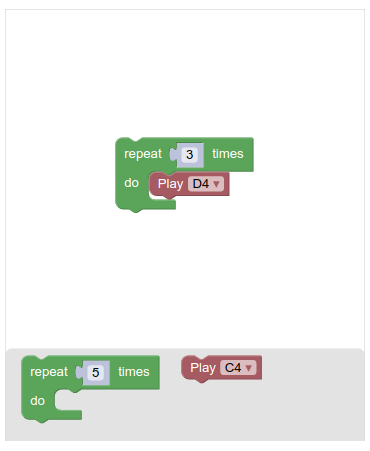
\includegraphics[width=\textwidth]{assets/blockly/d4_three_times.png}

    \small (a) Edición del programa mediante bloques
  \end{minipage}
  \hfill
  \begin{minipage}[t]{0.47\textwidth}
    \centering
    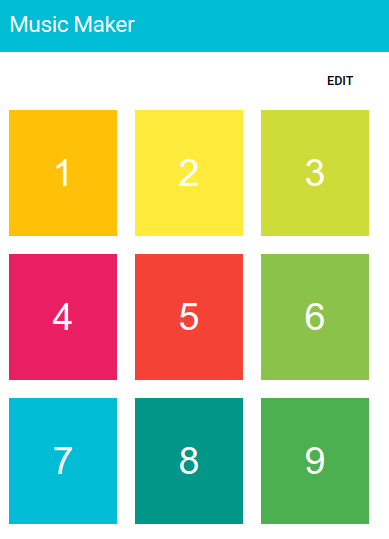
\includegraphics[width=\textwidth]{assets/blockly/play_mode.png}

    \small (b) Interfaz de reproducción de Music Maker
  \end{minipage}
  \caption{Edición y reproducción de un programa basado en bloques en Music
  Maker. Fuente: codelab oficial de Blockly \cite{blocklyGettingStartedCodelab}}
  \label{fig:blockly-music-maker}
\end{figure}

En este TFM, la programación por bloques se entiende como una sintaxis concreta
visual, es decir, como la forma visible con la que el usuario manipula un
lenguaje de dominio específico. El usuario final no necesita conocer la
implementación JavaScript del editor ni la estructura interna del metamodelo;
interactúa con un conjunto de bloques que representan conceptos del dominio.
Esta idea conecta directamente con la motivación del trabajo: crear lenguajes
de bloques para diferentes dominios sin programar manualmente cada editor desde
cero.

\section{Blockly}
\label{sec:blockly}

Blockly es una biblioteca web de código abierto para construir editores basados
en bloques. La documentación oficial describe Blockly como una biblioteca que
permite integrar un editor de código visual en una aplicación web; el
desarrollador define los bloques y la semántica asociada, mientras que la
biblioteca proporciona la infraestructura de interacción visual, arrastre,
encaje, paleta y serialización \cite{blocklyWhatIs,blocklyDocs}.

La biblioteca permite definir bloques con campos, entradas de valor, entradas
de sentencias, conexiones previas y posteriores, colores, tooltips y
generadores de código. También permite organizar los bloques en categorías de
paleta o \emph{toolbox}, y serializar el estado del área de trabajo o
\emph{workspace} \cite{blocklyGoogleDevelopers}. Estas capacidades hacen que
Blockly sea una base adecuada para construir lenguajes visuales específicos,
pero no eliminan la necesidad de definir manualmente la configuración de cada
dominio.

Antes de definir elementos específicos del dominio, el desarrollador debe
cargar las dependencias, proporcionar un contenedor HTML e inicializar el
espacio de trabajo. El Listado \ref{lst:blockly-infraestructura-minima} resume esta
infraestructura mínima siguiendo el codelab oficial
\cite{blocklyGettingStartedCodelab}.

\begin{lstlisting}[style=tfmhtml, caption={Infraestructura mínima para crear un espacio de trabajo Blockly}, label={lst:blockly-infraestructura-minima}]
<script src="https://unpkg.com/blockly/blockly_compressed.js"></script>
<script src="https://unpkg.com/blockly/blocks_compressed.js"></script>
<script src="https://unpkg.com/blockly/javascript_compressed.js"></script>
<script src="https://unpkg.com/blockly/msg/en.js"></script>

<div id="blocklyDiv"></div>

Blockly.inject("blocklyDiv", {"toolbox": toolbox});
\end{lstlisting}

El Listado \ref{lst:blockly-music-maker-config} muestra un ejemplo reducido de
esa configuración, tomado del codelab oficial Music Maker
\cite{blocklyGettingStartedCodelab}. El primer objeto define un bloque con un
campo desplegable para seleccionar una nota y con conexiones anterior y
posterior. El segundo determina qué tipos de bloque aparecen en la paleta.
Aunque se habla habitualmente de definiciones JSON, en este caso se expresan
como objetos JavaScript cuyos valores son serializables como JSON.

\begin{lstlisting}[style=tfmjavascript, caption={Definición de un bloque y configuración mínima de una paleta en Blockly}, label={lst:blockly-music-maker-config}]
Blockly.common.defineBlocksWithJsonArray([{
  "type": "play_sound",
  "message0": "Play %1",
  "args0": [{
    "type": "field_dropdown",
    "name": "VALUE",
    "options": [
      ["C4", "sounds/c4.m4a"],
      ["D4", "sounds/d4.m4a"]
    ]
  }],
  "previousStatement": null,
  "nextStatement": null,
  "colour": 355
}]);

const toolbox = {
  "kind": "flyoutToolbox",
  "contents": [
    {"kind": "block", "type": "controls_repeat_ext"},
    {"kind": "block", "type": "play_sound"}
  ]
};
\end{lstlisting}

La Figura \ref{fig:blockly-music-maker-toolbox} muestra el editor resultante: la
paleta ofrece el bloque de repetición y el bloque musical, que pueden
arrastrarse al espacio de trabajo para construir el programa.

\begin{figure}[htbp]
  \centering
  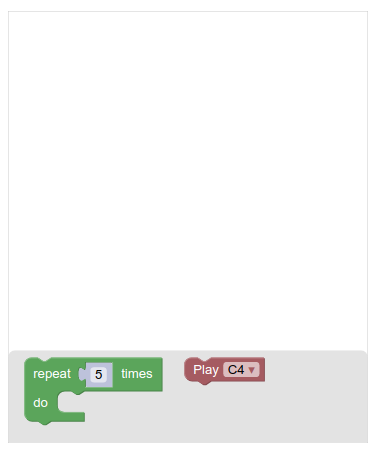
\includegraphics[width=0.48\textwidth]{assets/blockly/workspace_with_toolbox.png}
  \caption{Espacio de trabajo y paleta obtenidos tras registrar el bloque
  \texttt{play\_sound}. Fuente: codelab oficial de Blockly
  \cite{blocklyGettingStartedCodelab}}
  \label{fig:blockly-music-maker-toolbox}
\end{figure}

Aunque el editor resultante solo ofrece un bucle y una operación musical, su
construcción exige gestionar dependencias, preparar el contenedor, configurar
el espacio de trabajo y declarar manualmente la estructura, los campos, las conexiones y
la paleta. Todavía habría que añadir el generador de código y la lógica de
ejecución. Este esfuerzo crece con el número de conceptos y restricciones del
dominio y se repite para cada editor. La Figura
\ref{fig:blockly-music-maker}, presentada en la sección anterior, muestra cómo
el usuario combina posteriormente esos bloques para definir el comportamiento
de Music Maker.

El problema que aborda este TFM aparece precisamente en ese punto. Si se desea
crear un editor Blockly para un dominio de planificación, otro para un dominio
de storytelling y otro para un dominio de robótica, gran parte del trabajo se
repite: declarar bloques, campos, categorías, conexiones, validaciones y
generadores. El enfoque propuesto consiste en generar esos elementos a partir
de una descripción abstracta del dominio. Así, Blockly se utiliza como
plataforma de ejecución visual, pero la especificación del lenguaje se mantiene
en un nivel de metamodelo o DSL.

\section{Lenguajes de dominio específico e ingeniería dirigida por modelos}
\label{sec:dsml-mde}

Un lenguaje de dominio específico ofrece conceptos y notaciones adaptados a una
familia concreta de problemas. A diferencia de un lenguaje de propósito general,
un DSL permite usar términos propios del dominio. En enfoques basados en
metamodelado, un DSL suele tener una sintaxis abstracta, definida mediante un
metamodelo, y una o varias sintaxis concretas con las que trabaja el usuario
\cite{sal2024dsl,wasowski2023dsl}.

La ingeniería dirigida por modelos ofrece un marco para esta separación. En MDE,
los modelos son artefactos principales del desarrollo. Se usan para especificar,
diseñar, analizar, transformar y generar software \cite{brambilla2017modelDriven}.
En la industria, algunas motivaciones para usar MDE son reducir tiempo de
desarrollo, reutilizar soluciones y mejorar la calidad
\cite{brambilla2017modelDriven,hutchinson2014industry,akdur2018survey}.
Estas ideas encajan con este TFM: usar un generador para producir editores
Blockly en vez de programar cada editor desde cero.

En el ámbito del modelado, existen también estándares generales como UML y OCL.
UML define una notación gráfica estandarizada para visualizar, especificar,
construir y documentar sistemas software, mientras que OCL proporciona un
lenguaje formal para expresar restricciones sobre modelos \cite{omgUml,omgOcl}.
Estos estándares son relevantes como contexto, pero el presente TFM no propone
un perfil UML ni una integración completa de OCL. La decisión tomada es más
concreta: usar un metamodelo como descripción abstracta del dominio,
enriquecerlo con información sobre la sintaxis visual y derivar a partir de ella
una sintaxis concreta basada en bloques. En este trabajo, esta función se
implementa mediante Ecore, tecnología que se presenta en la Sección
\ref{sec:emf-ecore}.
El DSL textual del proyecto se entiende como una segunda ruta de autoría para
diseñadores de lenguajes: permite describir la estructura del editor Blockly de
forma más compacta y normalizarla al mismo modelo intermedio.

La experiencia acumulada en lenguajes específicos de dominio muestra además que
las herramientas de modelado pueden elevar el nivel de abstracción al expresar
soluciones directamente con conceptos del dominio y generar artefactos a partir
de esos modelos \cite{luoma2004dsm}. Esta idea coincide con la motivación de
Model2Blockly: que el usuario defina los conceptos del dominio y que la
infraestructura genere el editor visual correspondiente.

En este proyecto, la sintaxis basada en bloques se considera una sintaxis
concreta visual del dominio. El metamodelo Ecore describe qué conceptos existen
y cómo se relacionan; las anotaciones aportan información de presentación que
Ecore no expresa de forma nativa; la ruta textual \texttt{.m2b} puede escribir
la definición del lenguaje de bloques en un formato más breve. El generador
produce la configuración Blockly que implementa la sintaxis visual usada por el
usuario final.

\section{EMF y Ecore}
\label{sec:emf-ecore}

Eclipse Modeling Framework (EMF) es una infraestructura de modelado para definir
modelos estructurados y generar código a partir de ellos. Ecore es el
metamodelo central de EMF y permite representar paquetes, clases, atributos,
referencias, tipos de datos, herencia y cardinalidades
\cite{emfOverview,steinberg2008emf}. En la práctica, Ecore proporciona una
forma compacta y ampliamente utilizada de describir la estructura abstracta de
un dominio.

En este TFM, Ecore cumple tres funciones. Primero, describe la estructura del
dominio: las clases son conceptos, los atributos son propiedades y las
referencias son relaciones. Segundo, permite obtener información para la sintaxis
de bloques: una clase puede ser un tipo de bloque, un atributo puede ser un campo
y una referencia de contención puede ser una entrada para bloques hijos. Tercero,
Ecore permite añadir anotaciones de presentación, como etiquetas, colores,
categorías o tooltips.

La Figura \ref{fig:ecore-metamodelo-simplificado} representa el fragmento del
metamodelo Ecore relevante para estas funciones. Se omiten algunos tipos
intermedios, como \texttt{ENamedElement} y \texttt{ETypedElement}, para mantener
legible el diagrama.

\begin{figure}[H]
  \centering
  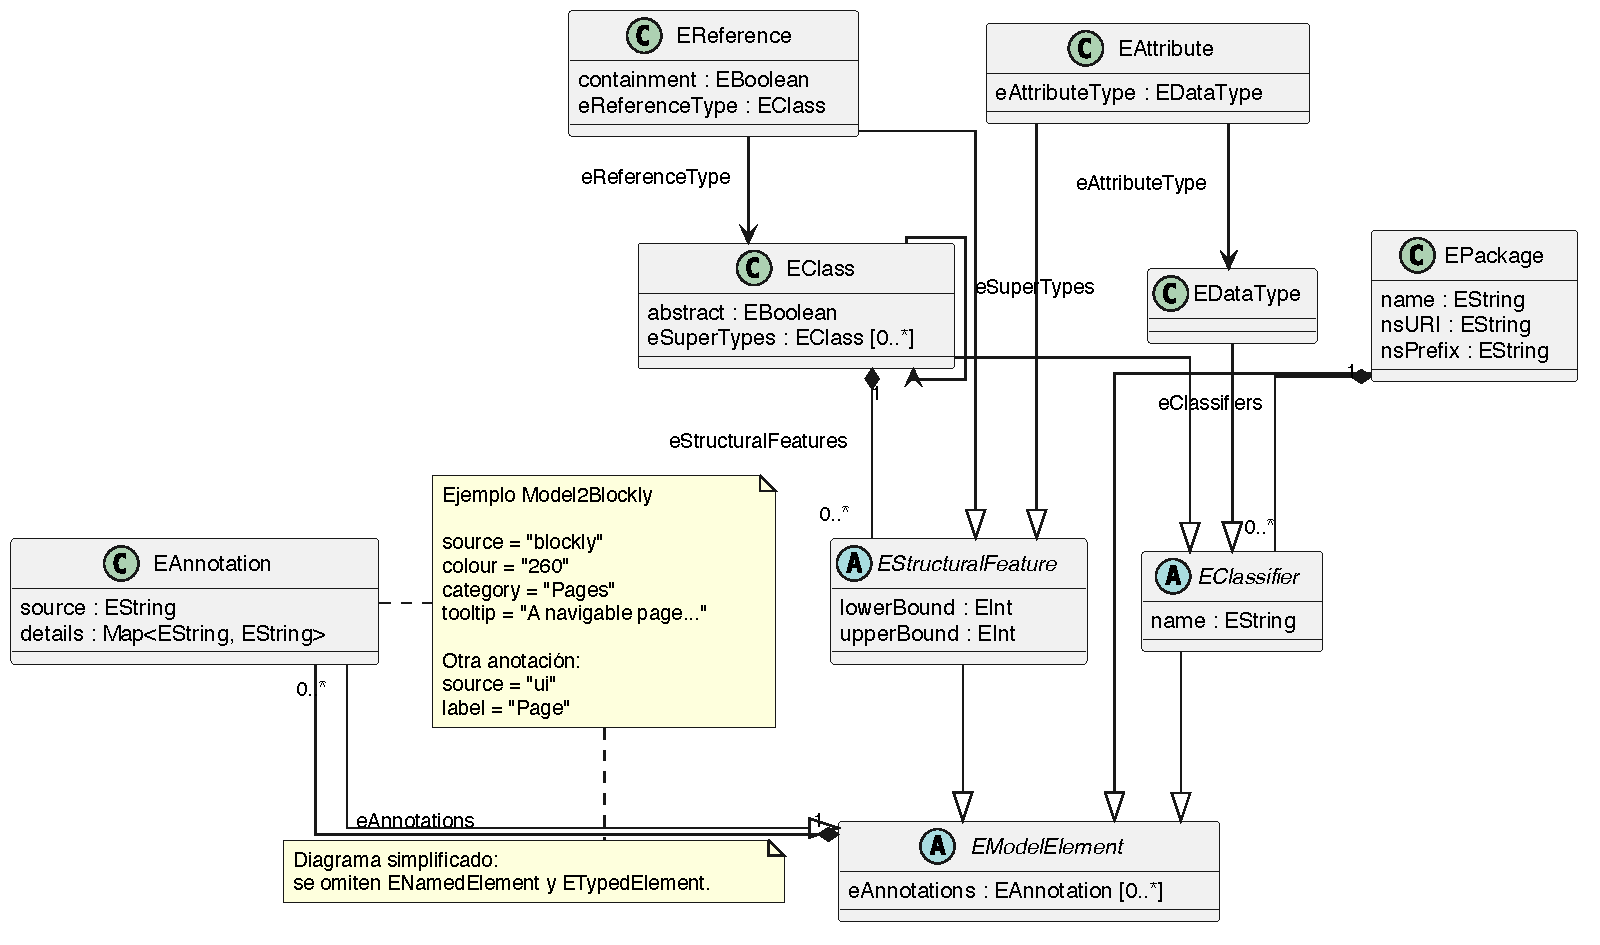
\includegraphics[width=\textwidth]{assets/uml/uml.pdf}
  \caption{Fragmento simplificado del metamodelo Ecore y uso de anotaciones en
  Model2Blockly}
  \label{fig:ecore-metamodelo-simplificado}
\end{figure}

Un \texttt{EPackage} agrupa los clasificadores del dominio. Entre ellos, una
\texttt{EClass} representa un concepto y puede contener características
estructurales: los \texttt{EAttribute} almacenan valores tipados y las
\texttt{EReference} relacionan instancias de clases, con la posibilidad de
marcar una relación como contención. Los límites inferior y superior expresan
la cardinalidad de cada característica. Estos elementos heredan, directa o
indirectamente, de \texttt{EModelElement}, que permite asociar instancias de
\texttt{EAnnotation}. Cada anotación identifica su propósito mediante
\texttt{source} y almacena pares clave--valor en \texttt{details}; Model2Blockly
utiliza este mecanismo para incorporar información de sintaxis visual sin
alterar la estructura abstracta del dominio. En el ejemplo de la figura, la
anotación con \texttt{source="blockly"} define \texttt{colour},
\texttt{category} y \texttt{tooltip}, mientras que una anotación separada con
\texttt{source="ui"} proporciona la etiqueta visible mediante \texttt{label}.

Esta capacidad de separar estructura e información de presentación es esencial
para el trabajo. No todos los detalles de un editor Blockly existen de forma
natural en un metamodelo Ecore: por ejemplo, el color de un bloque o la
organización de la paleta son decisiones de sintaxis concreta. Por ello, el
proyecto permite enriquecer el metamodelo con anotaciones específicas, sin
perder la posibilidad de generar un editor básico a partir de la estructura
Ecore.

\section{Xtext}
\label{sec:xtext}

Xtext es un framework de Eclipse para el desarrollo de lenguajes textuales
específicos de dominio. A partir de una gramática, Xtext genera infraestructura
de análisis sintáctico, un modelo abstracto basado en EMF y soporte de edición
como resaltado de sintaxis, navegación, autocompletado y marcadores de error
\cite{xtextProject,bettini2013xtext,bettini2015xsemantics}. Estas
características lo hacen adecuado para construir una ruta textual alternativa a
la edición directa de metamodelos Ecore.

Conviene distinguir dos momentos en el funcionamiento de Xtext. En primer
lugar, durante la construcción de la herramienta, el desarrollador escribe una
gramática que describe las palabras clave, las reglas y las referencias del
lenguaje. Xtext procesa esa gramática y genera el analizador, la infraestructura
EMF y los servicios del editor. En segundo lugar, durante el uso de la
herramienta, ese analizador lee cada fichero escrito en el nuevo lenguaje y
construye una instancia de su modelo abstracto. Por lo tanto, Xtext no genera el
editor Blockly directamente: genera la infraestructura que permite comprender
una especificación textual, que después Model2Blockly transforma.

La Figura \ref{fig:funcionamiento-general-xtext} resume este mecanismo. La
gramática determina qué textos son válidos y cómo se relacionan con los
conceptos del modelo. A partir de ella se obtienen el parser y los servicios de
edición. Cuando el autor escribe una especificación, el parser construye un
grafo de objetos EMF; el enlazado resuelve nombres que hacen referencia a otros
elementos y el validador comunica los problemas detectados. Una transformación
posterior puede entonces consumir ese modelo sin volver a interpretar el texto.

\begin{figure}[htbp]
  \centering
  \resizebox{\textwidth}{!}{%
  \begin{tikzpicture}[
      node distance=0.75cm and 0.38cm,
      box/.style={draw=black!55, rounded corners=2pt, minimum width=2.18cm,
        minimum height=0.92cm, align=center, font=\small, inner sep=5pt},
      sourcebox/.style={box, fill=green!8},
      xtextbox/.style={box, fill=blue!7},
      commonbox/.style={box, fill=orange!10},
      arrow/.style={-{Latex[length=2.4mm]}, thick, draw=black!70},
      control/.style={-{Latex[length=2.2mm]}, dashed, thick, draw=black!55}
    ]
    \node[sourcebox] (dsl) {Especificación\\textual \texttt{.m2b}};
    \node[xtextbox, right=of dsl] (parser) {Parser, enlazado\\y validación};
    \node[xtextbox, right=of parser] (model) {Modelo abstracto\\basado en EMF};
    \node[commonbox, right=of model] (transformation)
      {Transformación de\\Model2Blockly};
    \node[commonbox, right=of transformation] (editor)
      {Editor Blockly\\generado};
    \node[sourcebox, above=0.55cm of parser] (grammar) {Gramática Xtext};

    \draw[control] (grammar.south) -- (parser.north);
    \draw[arrow] (dsl) -- (parser);
    \draw[arrow] (parser) -- (model);
    \draw[arrow] (model) -- (transformation);
    \draw[arrow] (transformation) -- (editor);
  \end{tikzpicture}%
  }
  \caption{Funcionamiento general de Xtext y su aplicación en Model2Blockly}
  \label{fig:funcionamiento-general-xtext}
\end{figure}

En este proyecto, Xtext se usa para definir el lenguaje textual
\texttt{.m2b}. El Listado \ref{lst:xtext-m2b-breve} ilustra su nivel de
abstracción: el autor declara conceptos del dominio, propiedades y relaciones,
en lugar de programar directamente llamadas a la API JavaScript de Blockly.

\begin{lstlisting}[style=tfmm2b, caption={Ejemplo breve de una definición textual \texttt{.m2b}}, label={lst:xtext-m2b-breve}]
// Define el nombre del dominio que se transformara.
domain BasicStructure
// Declara una clase concreta y desactiva los campos en linea.
class Board inputsInline false {
  // Define un atributo de texto opcional con valor inicial.
  attribute name : string [0..1] default "Sprint board"
  // Expresa una contencion de uno a cuatro elementos.
  contains WorkItem items [1..4]
} // Finaliza la declaracion de Board.
// Declara el tipo abstracto usado por la contencion.
abstract class WorkItem inputsInline false {
} // Finaliza la declaracion de WorkItem.
\end{lstlisting}

La declaración \texttt{class Board} representa un concepto que podrá convertirse
en un tipo de bloque; \texttt{name} aporta una propiedad editable e
\texttt{items} expresa una relación jerárquica con cardinalidad. Xtext
comprueba que la entrada respeta la gramática y que nombres como
\texttt{Board} y \texttt{WorkItem} se pueden resolver. El resultado es un
modelo EMF que la cadena de Model2Blockly puede transformar posteriormente.
Este mecanismo concreto se desarrolla desde el punto de vista arquitectónico
en la Sección \ref{sec:ruta-xtext} y desde el punto de vista de implementación
en la Sección \ref{sec:implementacion-xtext}.

La ruta Xtext no sustituye, por lo tanto, a la ruta Ecore; la complementa. Ecore
resulta adecuado cuando ya existe un metamodelo EMF o cuando se quiere mantener
la definición del dominio dentro de dicho ecosistema. La ruta \texttt{.m2b}
resulta útil cuando se desea reunir en un fichero legible la estructura del
dominio y las decisiones de sintaxis concreta, como etiquetas, colores,
widgets, organización de la paleta y plantillas de código. La convergencia en
\texttt{EditorSpec} evita mantener dos generadores diferentes.

\section{Xtend}
\label{sec:xtend}

Xtend es un lenguaje de programación estáticamente tipado del ecosistema Xtext.
Su sintaxis parte de Java, pero añade construcciones más concisas, como
inferencia de tipos, métodos de extensión, expresiones lambda, expresiones
\texttt{switch} y plantillas de texto. El compilador de Xtend traduce los
ficheros \texttt{.xtend} a código fuente Java, por lo que el código resultante se
ejecuta sobre la JVM y puede utilizar directamente clases y bibliotecas Java
\cite{xtendDocs}.

Para la generación de código resultan especialmente útiles las expresiones de
plantilla. Una plantilla se delimita mediante triples comillas simples y permite
insertar expresiones entre los caracteres \texttt{«} y \texttt{»}. Xtend evalúa
esas expresiones, incorpora su representación textual y aplica reglas de
indentación que ayudan a mantener legibles tanto la plantilla como la salida
generada \cite{xtendDocs}. El Listado \ref{lst:xtend-plantilla} muestra un
fragmento simplificado, basado en el generador del proyecto.

\begin{lstlisting}[style=tfmxtend, caption={Ejemplo de una plantilla Xtend usada para generar JavaScript}, label={lst:xtend-plantilla}]
def String generateBlocksJs(EditorSpec spec) '''
  // Block definitions for domain "«spec.domainName»".
  window.BLOCKLY_BLOCKS = «generateBlocksArray(spec)»;
'''
\end{lstlisting}

En el ejemplo, \texttt{def} declara un método y la plantilla constituye su
resultado. Las expresiones insertadas obtienen el nombre del dominio y la lista
de bloques calculada por otro método. El mismo mecanismo permite combinar texto
HTML o JavaScript con recorridos, condiciones y datos procedentes de un modelo
EMF, sin construir la salida mediante numerosas concatenaciones de cadenas.

Dentro de Model2Blockly, Xtend no define el lenguaje \texttt{.m2b} ni forma
parte del editor generado. Se utiliza como tecnología de implementación en dos
puntos: \texttt{Model2Blockly}\allowbreak\texttt{Generator} integra la
generación con el flujo de Xtext, y
\texttt{BlocklyCode}\allowbreak\texttt{Generator} contiene las transformaciones y
plantillas que producen bloques, paleta, validaciones y páginas HTML. Gracias
a la interoperabilidad con Java, estas clases invocan los adaptadores,
serializadores y utilidades Java del proyecto, y también pueden ser invocadas
desde las entradas independientes escritas en Java. Los detalles de esta
implementación se presentan en la Sección
\ref{sec:implementacion-generador-html}.

\section{Trabajos relacionados sobre DSLs basados en bloques}
\label{sec:trabajos-relacionados-block-dsl}

Además de las tecnologías utilizadas, existen trabajos que tratan de reducir el
esfuerzo de construir lenguajes basados en bloques. Pasternak, Fenichel y
Marshall describen recomendaciones prácticas para crear lenguajes con Blockly:
decidir el estilo de los bloques, seleccionar qué conceptos deben ser visibles y
mantener la complejidad de la API alejada del usuario final
\cite{pasternak2017tips}. Este trabajo es relevante porque muestra que Blockly
es flexible, pero también que diseñar un lenguaje de bloques implica decisiones
de ingeniería que no desaparecen al usar la biblioteca.

Merino y van der Storm plantean el problema desde la perspectiva de los
\emph{language workbenches}: la creación de lenguajes de bloques sigue siendo a
menudo una tarea de bajo nivel y debería poder abordarse con metalenguajes y
herramientas específicas \cite{verano2018workbenchBlocks}. En una línea
posterior, Kogi deriva entornos de bloques desde gramáticas libres de contexto y
define una estructura intermedia para describir el entorno generado
\cite{verano2020kogi}. Blocklybench propone un entorno basado en bloques para
describir otros entornos de bloques, incluyendo aspectos como disposición,
colores, conexiones y generación de código \cite{verano2022blocklybench}.

Model2Blockly se sitúa cerca de estos trabajos porque también busca elevar el
nivel de abstracción al crear editores de bloques. La diferencia principal está
en la fuente de información: en lugar de partir de gramáticas textuales libres de
contexto o de un metaeditor de bloques, esta propuesta admite metamodelos Ecore
anotados y modelos textuales \texttt{.m2b}. Ambas rutas convergen en un modelo
intermedio definido explícitamente como metamodelo EMF, para mantener una cadena
MDE entre la transformación de entrada y el generador HTML/JavaScript.

\section{Comparación y posicionamiento de la propuesta}
\label{sec:comparacion-posicionamiento}

Las tecnologías anteriores cubren partes distintas del problema, pero ninguna
resuelve por sí sola el objetivo de este TFM. Blockly ofrece la infraestructura
de bloques, pero exige configurar cada dominio a mano. EMF/Ecore describe la
estructura abstracta de un dominio, pero no genera un editor de bloques. Xtext
ayuda a crear lenguajes textuales, pero su salida natural no es un editor
Blockly. UML y OCL son referencias importantes para modelado y restricciones,
pero este trabajo se centra en una cadena generativa más concreta.

La Tabla \ref{tab:comparacion-enfoques} resume esta comparación y sitúa el papel
de Model2Blockly dentro del contexto revisado. La propuesta no pretende reemplazar
estas tecnologías, sino conectarlas mediante una representación intermedia que
permita derivar una sintaxis concreta visual desde una descripción de dominio.

\begin{table}[h]
  \centering
  \small
  \begin{tabular}{|L{0.24\textwidth}|L{0.30\textwidth}|L{0.34\textwidth}|}
    \hline
    Enfoque & Aportación principal & Limitación respecto al objetivo del TFM \\
    \hline
    Desarrollo manual con Blockly & Permite construir editores visuales ricos y
    ejecutables en la web. & Requiere codificar bloques, paleta, conexiones,
    validaciones y generadores para cada dominio. \\
    Metamodelado con Ecore & Define de forma precisa la estructura abstracta del
    dominio. & No produce automáticamente una sintaxis concreta basada en
    bloques. \\
    Sintaxis textual con Xtext & Genera infraestructura de lenguaje textual,
    validación y edición. En este TFM se usa para la ruta \texttt{.m2b}. &
    No convierte por sí sola esa definición en un editor visual Blockly. \\
	    Restricciones generales con OCL & Expresa propiedades formales sobre modelos.
	    & Supera el alcance de las validaciones estructurales generadas en este
	    trabajo. \\
    Kogi y Blocklybench & Generan o describen entornos de bloques desde
    artefactos de lenguaje o metaentornos específicos. & No toman como fuente
    principal metamodelos Ecore anotados ni usan un \texttt{EditorSpec} EMF como
    contrato XMI explícito para la generación. \\
	    Model2Blockly & Conecta metamodelos Ecore anotados y modelos
	    \texttt{.m2b} con editores Blockly mediante transformación, modelo
	    intermedio y generación. & Su evaluación cubre un corpus intencional y no
    reproduce todavía todas las políticas de conexión, paletas programáticas ni
    generadores con estado. \\
    \hline
  \end{tabular}
  \caption{Posicionamiento de Model2Blockly frente a enfoques relacionados}
  \label{tab:comparacion-enfoques}
\end{table}

\section{Relación entre las tecnologías}
\label{sec:relacion-tecnologias}

La relación entre las tecnologías utilizadas puede resumirse como una cadena de
transformación. EMF/Ecore permite definir la estructura abstracta del dominio y
las anotaciones añaden metadatos de sintaxis concreta. Xtext ofrece la ruta
textual \texttt{.m2b} para escribir definiciones compactas de lenguajes de
bloques. Blockly proporciona la
infraestructura web para ejecutar la sintaxis visual basada en bloques. El
generador desarrollado en Java y Xtend conecta estos elementos mediante un
modelo intermedio EMF independiente de la salida final; Xtend se emplea
principalmente para expresar las plantillas textuales de la salida.

La Tabla \ref{tab:tecnologias-papel} resume el papel de cada tecnología dentro
del proyecto.

\begin{table}[h]
  \centering
  \begin{tabular}{|p{0.22\textwidth}|p{0.66\textwidth}|}
    \hline
    Tecnología & Papel en el TFM \\
    \hline
    Blockly & Plataforma web para representar bloques, paleta, espacio de trabajo,
    conexiones y generación asociada. \\
    EMF/Ecore & Definición estructural del dominio mediante metamodelos,
    clases, atributos, referencias y cardinalidades. \\
    Xtext & Ruta textual \texttt{.m2b} para definir lenguajes de bloques y
    generar modelos EMF a partir de descripciones compactas. \\
    Java & Implementación de adaptadores, validadores, serialización del modelo
    intermedio y utilidades de ejecución. \\
    Xtend & Implementación del punto de entrada de generación de Xtext y de las
    plantillas que producen los artefactos HTML/JavaScript. \\
    HTML/JavaScript & Tecnología de salida principal para ejecutar el editor
    Blockly generado en el navegador. \\
    \hline
  \end{tabular}
  \caption{Papel de las tecnologías principales en el proyecto}
  \label{tab:tecnologias-papel}
\end{table}

Esta combinación da soporte técnico al enfoque del proyecto: definir lenguajes
de dominio específico a un nivel abstracto y generar automáticamente una
sintaxis concreta basada en bloques. El valor de la solución no reside en usar
Blockly de forma aislada, sino en integrarlo con metamodelado Ecore,
transformación de modelos y generación para crear editores reutilizables en
distintos dominios.

\chapter{Diseño y arquitectura de la solución}
\label{chap:diseno-arquitectura}

La arquitectura de Model2Blockly considera que un editor Blockly es una sintaxis
visual de un lenguaje de dominio específico. Por eso, el sistema debe partir de
una descripción abstracta del dominio y producir una implementación web ejecutable.

El capítulo se organiza de la siguiente manera. En primer lugar, se presenta el
enfoque arquitectónico y el flujo general de generación. A continuación, se
describe el modelo intermedio que conecta las entradas con los generadores.
Después se justifican las rutas basadas en Ecore y en el DSL textual
\texttt{.m2b}, así como la generación de los editores Blockly. Finalmente, se
exponen los mecanismos de validación, referencias y personalización, y se
relacionan las decisiones arquitectónicas con los objetivos del trabajo.

\section{Enfoque general}
\label{sec:enfoque-arquitectonico}

La arquitectura del sistema sigue un enfoque de ingeniería dirigida por modelos.
En lugar de definir manualmente cada bloque en JavaScript, el diseñador describe
el dominio mediante un metamodelo Ecore anotado o mediante una definición
textual \texttt{.m2b}. A partir de esa descripción, Model2Blockly deriva la
estructura y parte del comportamiento del editor. Esta organización aplica los
principios de MDE al diseño concreto de la solución: los modelos constituyen la
entrada principal del proceso y se utilizan para generar software
\cite{brambilla2017modelDriven}.

En ambas rutas se mantiene la separación habitual entre sintaxis abstracta y
sintaxis concreta de un DSL \cite{sal2024dsl}. Ecore o el lenguaje
\texttt{.m2b} describen los conceptos y relaciones del dominio, mientras que
Blockly proporciona la notación visual con la que el usuario final crea y edita
instancias. Por lo tanto, el lenguaje textual de Xtext no sustituye al editor
visual: es una forma compacta de especificar qué lenguaje de bloques debe
generarse.

El diseño se apoya en tres principios. El primero es separar la interpretación
del dominio de la generación del editor. El segundo es hacer que las dos rutas
de entrada produzcan un modelo \texttt{EditorSpec} conforme al mismo metamodelo
intermedio. Este modelo constituye el contrato arquitectónico compartido antes
de generar HTML y JavaScript. El tercero es derivar no solo la apariencia de los
bloques, sino también parte de su comportamiento: conexiones, validaciones,
referencias, exportación y metadatos de interfaz.

Estos principios responden al problema identificado en la introducción. Blockly
proporciona la infraestructura de interacción visual, pero exige que el
desarrollador describa cada bloque, campo, conexión y generador
\cite{blocklyDocs}. Model2Blockly desplaza esa descripción a un nivel de dominio:
el desarrollador define clases, atributos, contenciones, referencias,
anotaciones o construcciones textuales \texttt{.m2b}; la herramienta se encarga
de transformar esa información en los artefactos Blockly correspondientes.

\section{Flujo general de generación}
\label{sec:flujo-generacion}

El flujo completo de la solución se organiza en cuatro etapas:

\begin{enumerate}
  \item definición del dominio mediante un metamodelo Ecore con anotaciones o
  mediante un fichero textual \texttt{.m2b};
  \item interpretación de la entrada y transformación a un modelo intermedio
  común;
  \item generación de los artefactos Blockly a partir de ese modelo;
  \item ejecución del editor generado en el navegador.
\end{enumerate}

La Figura \ref{fig:arquitectura-general} muestra las dos rutas de entrada y la
cadena común que se ejecuta después de convertirlas al modelo intermedio.

\begin{figure}[H]
  \centering
  \begin{tikzpicture}[
      node distance=0.75cm and 2.2cm,
      box/.style={draw=black!55, rounded corners=2pt, minimum width=3.65cm,
        minimum height=0.92cm, align=center, font=\small, inner sep=5pt},
      inputbox/.style={box, fill=green!8},
      stagebox/.style={box, fill=blue!7},
      commonbox/.style={box, fill=orange!10},
      outputbox/.style={box, fill=orange!10},
      arrow/.style={-{Latex[length=2.5mm]}, thick, draw=black!70}
    ]
    \node[inputbox] (ecore) {Metamodelo Ecore\\anotado};
    \node[inputbox, right=of ecore] (dsl) {Definición textual\\\texttt{.m2b}};

    \node[stagebox, below=of ecore] (ecoreAdapter)
      {Transformación del\\modelo Ecore};
    \node[stagebox, below=of dsl] (xtextPath)
      {Análisis Xtext y transformación\\del modelo textual};

    \path let \p1=(ecoreAdapter), \p2=(xtextPath) in
      node[commonbox] (editorSpec) at ($ (\p1)!0.5!(\p2) +(0,-1.7cm) $)
      {Modelo intermedio común\\\texttt{EditorSpec}};
    \node[commonbox, below=of editorSpec] (generator)
      {Generación de artefactos\\Blockly};
    \node[outputbox, below=of generator] (outputs)
      {Editor Blockly ejecutable\\HTML/JavaScript};

    \draw[arrow] (ecore) -- (ecoreAdapter);
    \draw[arrow] (dsl) -- (xtextPath);
    \draw[arrow] (ecoreAdapter) -- (editorSpec);
    \draw[arrow] (xtextPath) -- (editorSpec);
    \draw[arrow] (editorSpec) -- (generator);
    \draw[arrow] (generator) -- (outputs);
  \end{tikzpicture}
  \caption{Arquitectura general de la generación de editores Blockly}
  \label{fig:arquitectura-general}
\end{figure}

La Figura \ref{fig:arquitectura-general} muestra dos recorridos diferentes en su
parte superior. En la ruta Ecore se interpreta la estructura del metamodelo y
sus anotaciones para construir el modelo intermedio. En la ruta textual, Xtext
analiza primero la definición \texttt{.m2b} y crea un modelo estructurado; una
segunda transformación lleva ese modelo a \texttt{EditorSpec}. Las dos rutas
terminan, por lo tanto, en modelos conformes al mismo metamodelo intermedio.

Por ejemplo, una \texttt{EClass Page} con un atributo
\texttt{title:EString} y una declaración textual \texttt{class Page} con
\texttt{attribute title:string} se representan de la misma forma después de la
conversión: un tipo de bloque \texttt{Page} con un campo de texto
\texttt{title}. Desde ese punto se aplica una única generación sobre
\texttt{EditorSpec}. Por ello, la solución necesita dos mecanismos de entrada,
pero comparte la representación intermedia y la generación de salida. Esta
convergencia es la decisión que estructura el resto de la arquitectura.

\section{Modelo intermedio}
\label{sec:modelo-intermedio}

Las dos rutas de entrada describen conceptos similares mediante representaciones
diferentes. Si la generación trabajara directamente con ambas, tendría que
mantener dos interpretaciones de clases, propiedades, relaciones y restricciones.
La incorporación de una nueva forma de entrada obligaría además a modificar la
generación. Para evitar esta dependencia, la arquitectura introduce un modelo
intermedio común entre las entradas y la salida.

Este modelo representa el editor que se desea obtener, no una copia completa del
artefacto de origen. Su contenido se organiza conceptualmente en tres grupos. El
primero describe la estructura general del editor, como las categorías de la
toolbox y su configuración. El segundo define los bloques, sus campos y sus
formas de conexión. El tercero conserva la información de comportamiento que
afecta a la edición, como referencias y reglas de validación. El metamodelo
intermedio establece las relaciones válidas entre estos conceptos y cada
transformación de entrada produce un modelo conforme a él.

La raíz de esta representación se denomina \texttt{EditorSpec}. Por ejemplo,
una clase de dominio \texttt{Page} se representa como un tipo de bloque y su
propiedad \texttt{title} como un campo editable. Una relación de composición se
representa como una zona para insertar bloques hijos, mientras que una referencia
a otro objeto se representa como un mecanismo de selección. El origen puede ser
Ecore o \texttt{.m2b}; después de la transformación, estos conceptos tienen la
misma forma para la generación.

% Cuando esté disponible el diagrama UML definitivo exportado desde PlantUML,
% insertarlo aquí con las clases, atributos, roles, multiplicidades y relaciones
% de contención del metamodelo intermedio.

La elección de esta representación intermedia permite que cada parte tenga una
responsabilidad definida. Las rutas de entrada interpretan el dominio y la
generación interpreta únicamente \texttt{EditorSpec}. Así se comparte una sola
lógica de salida y se pueden modificar o ampliar las entradas sin rediseñar el
proceso que produce el editor Blockly.

\section{Ruta basada en Ecore}
\label{sec:ruta-ecore}

La ruta Ecore está dirigida a dominios que ya se encuentran definidos dentro
del ecosistema EMF. Permite reutilizar un metamodelo existente como punto de
partida, en lugar de volver a describir manualmente sus conceptos para Blockly.
Ecore aporta la estructura abstracta del dominio mediante clases, atributos,
referencias, herencia y cardinalidades \cite{emfOverview}.

El mapeo básico es sistemático. Cada clase Ecore se convierte en un tipo de
bloque; cada atributo, en un campo visual; cada referencia de contención, en una
entrada estructural para bloques hijos; y cada referencia no contenida, en un
campo de referencia dinámica. La herencia se utiliza para mantener la
compatibilidad entre tipos de bloque y las cardinalidades permiten derivar
comprobaciones sobre elementos obligatorios o cantidades admitidas. Estas reglas
de correspondencia preservan en el editor las diferencias estructurales que son
relevantes para crear modelos válidos.

Ecore no describe por sí solo todas las decisiones de sintaxis concreta de un
editor Blockly, como el color, la etiqueta visible, la organización de la
toolbox o el tipo de control utilizado para editar un valor. Por este motivo, la
ruta admite anotaciones que complementan el metamodelo sin alterar su estructura
esencial. La separación entre estructura del dominio y metadatos de presentación
permite obtener una salida útil por defecto y personalizarla cuando el dominio
lo requiere.

\section{Ruta textual \texttt{.m2b} basada en Xtext}
\label{sec:ruta-xtext}

La ruta textual ofrece una alternativa de autoría cuando no se dispone de un
metamodelo Ecore previo o se prefiere una notación más compacta. Xtext resulta
adecuado porque permite definir una sintaxis textual y obtener a partir de ella
una representación estructurada del dominio \cite{xtextProject,bettini2013xtext}.

Esta ruta no reemplaza a Ecore, sino que responde a una necesidad distinta. El
DSL permite reunir en una misma descripción la estructura del dominio y las
decisiones básicas de presentación del editor. Xtext se encarga de interpretar
el texto y comprobar que respeta la sintaxis definida; posteriormente, esa
representación se transforma al mismo modelo intermedio empleado por la ruta
Ecore. La generación continúa siendo común y no depende de la forma elegida para
describir el dominio.

\section{Generación de editores Blockly}
\label{sec:generacion-editores}

Una vez construido el modelo intermedio, la generación produce los artefactos
necesarios para ejecutar el editor en un navegador. Esta etapa puede entenderse
como una transformación de modelo a texto: la especificación del editor se
convierte en definiciones de bloques, toolbox, configuración del workspace,
reglas de validación y páginas HTML y JavaScript.

La correspondencia se establece por responsabilidad: la organización del modelo
intermedio determina la toolbox, la definición de cada tipo determina la forma
del bloque y sus conexiones, y las reglas conservadas determinan las ayudas y
advertencias disponibles durante la edición. Así, la salida visual se deriva de
decisiones expresadas en el modelo y no de una colección de bloques programados
manualmente.

La dependencia exclusiva respecto al modelo intermedio evita duplicar la lógica
de salida para cada entrada y deja abierta la posibilidad de incorporar otros
formatos de origen o nuevos objetivos de generación. Para este trabajo se elige
como salida principal un editor HTML/JavaScript autocontenido, porque facilita
su ejecución y revisión sin exigir una infraestructura adicional.

\section{Validaciones, referencias y personalización}
\label{sec:validaciones-referencias-personalizacion}

Un editor de bloques no debe limitarse a mostrar piezas visuales; también debe
ayudar a construir modelos coherentes. Por ello, la arquitectura conserva en el
modelo intermedio las restricciones que pueden trasladarse al editor. Entre
ellas se encuentran las cardinalidades, la obligatoriedad de valores y algunas
relaciones sencillas entre elementos. La decisión de mantenerlas en el modelo
intermedio permite aplicar el mismo criterio de validación con independencia de
la ruta de entrada.

Estas comprobaciones no constituyen un motor general de restricciones. OCL
permite expresar invariantes sobre objetos, propiedades y colecciones
\cite{omgOcl}, mientras que Model2Blockly solo transforma patrones que pueden
reconocerse y ejecutarse de manera predecible en el editor generado. Esta
decisión mantiene explícito el alcance del sistema: las validaciones ayudan al
usuario mediante advertencias, pero no sustituyen a un lenguaje completo de
restricciones. La implementación concreta y la evaluación del subconjunto
soportado se presentan en los capítulos siguientes.

Las referencias no contenidas se tratan de forma distinta a las contenciones.
Una contención define la estructura jerárquica del modelo y por lo tanto se
representa como una entrada de sentencias. Una referencia no contenida apunta a
otro elemento existente en el workspace, por lo que se representa mediante un
desplegable dinámico. El generador calcula los candidatos compatibles teniendo
en cuenta el tipo objetivo y sus subtipos. Esta decisión mantiene una
diferencia semántica importante del metamodelo: no es lo mismo crear un hijo
estructural que seleccionar otro elemento ya presente en el modelo.

La personalización se incorpora como una capa controlada de metadatos. Colores,
etiquetas, categorías, tooltips, disposición en línea, widgets de interfaz y
plantillas de código no cambian la estructura esencial del dominio, pero sí
afectan a la experiencia del usuario final. Model2Blockly permite definir esta
información mediante anotaciones Ecore o mediante opciones del DSL textual. De
este modo, se evita que el usuario tenga que editar directamente JavaScript para
realizar cambios habituales de presentación.

\section{Trazabilidad con los objetivos}
\label{sec:trazabilidad-objetivos}

La arquitectura propuesta mantiene una relación directa con los objetivos
específicos definidos para el TFM. La Tabla
\ref{tab:trazabilidad-arquitectura} resume esa relación.

\begin{table}[h]
  \centering
  \begin{tabular}{|p{0.18\textwidth}|p{0.70\textwidth}|}
    \hline
    Objetivo & Respuesta arquitectónica \\
    \hline
    OE1 & El modelo intermedio identifica explícitamente los elementos que
    necesita un editor de bloques: tipos, campos, conexiones, categorías,
    referencias y validaciones. \\
    OE2 & La ruta Ecore permite partir de metamodelos y
    derivar bloques, campos, entradas y reglas. \\
    OE3 & La gramática Xtext proporciona la ruta textual \texttt{.m2b}
    para definir lenguajes de bloques de forma compacta. \\
    OE4 & El modelo intermedio común desacopla las entradas de los generadores
    y permite compartir la misma lógica de salida. \\
    OE5 & Los generadores producen editores HTML/JavaScript ejecutables en el
    navegador. \\
    OE6 & Las validaciones, referencias dinámicas, anotaciones de interfaz y
    plantillas de código se incorporan como capacidades genéricas. \\
    OE7 & La separación por transformación de entrada, modelo intermedio y
    generadores facilita probar cada parte y evaluar la convergencia de las dos
    rutas sobre AppMaker. \\
    \hline
  \end{tabular}
  \caption{Trazabilidad entre objetivos y arquitectura}
  \label{tab:trazabilidad-arquitectura}
\end{table}

En conjunto, la arquitectura define una cadena generativa clara: el diseñador
describe un dominio como metamodelo Ecore anotado o como fichero \texttt{.m2b},
el sistema transforma esa descripción en un modelo intermedio y el generador
produce un editor Blockly. La aportación principal no es un bloque concreto,
sino el mecanismo reutilizable que permite generar editores desde descripciones
de dominio de alto nivel.

\chapter{Implementación de Model2Blockly}
\label{chap:implementacion}

Este capítulo explica la implementación de Model2Blockly siguiendo el recorrido
de una ejecución completa. A diferencia del capítulo anterior, centrado en el
diseño y la arquitectura, aquí se identifican las tecnologías, clases y
operaciones que materializan cada etapa de la cadena generativa.

La exposición comienza mostrando cómo ejecutar la herramienta sobre el ejemplo
AppMaker y cómo localizar el editor obtenido. Después se presentan el flujo
interno, la organización del código y la carga y validación de las dos entradas.
Sobre esa base se detallan la ruta textual \texttt{.m2b}, el contrato y la
serialización del modelo intermedio \texttt{EditorSpec}, los adaptadores Java, el
generador HTML/JavaScript y el comportamiento en el navegador. El capítulo
termina con la integración y distribución en Eclipse, las entradas independientes y
las pruebas de implementación.

\section{Ejecución de Model2Blockly}
\label{sec:ejecucion-model2blockly}

Antes de detallar las clases internas, esta sección presenta el procedimiento
observable desde el punto de vista del usuario. La forma principal de ejecutar
Model2Blockly es mediante su plugin de Eclipse. El entorno debe iniciarse con
Java 21 y el plugin puede instalarse desde el repositorio p2 publicado por el
proyecto o ejecutarse desde el código fuente mediante una instancia runtime de
Eclipse. En ambos casos, la acción de generación se aplica a un fichero de
entrada situado en el workspace.

El ejemplo AppMaker incluido en el repositorio permite reproducir la ruta Ecore
mediante los siguientes pasos:

\begin{enumerate}
  \item abrir o importar el proyecto principal en Eclipse;
  \item seleccionar el fichero \path{model/app_maker.ecore};
  \item ejecutar \texttt{Model2Blockly -> Generate Blockly Editor} desde el menú
  contextual;
  \item revisar el informe \path{app_maker_generated/generation_report.html}
  que Eclipse abre al finalizar la generación;
  \item abrir
  \path{app_maker_generated/html/Appmaker_standalone.html} en un navegador para
  utilizar el editor generado.
\end{enumerate}

La ruta textual se ejecuta de la misma forma seleccionando
\path{examples/app_maker.m2b}. En los dos casos, si no se detectan errores, la
herramienta crea junto a la entrada un directorio con el sufijo
\texttt{\_generated}. El directorio contiene el informe de generación, una
serialización XMI de \texttt{EditorSpec}, las definiciones de bloques, la paleta,
los scripts de generación y validación, un modelo de ejemplo y las páginas HTML
del editor.

La Figura \ref{fig:appmaker-ecore-generation-report} muestra el informe que se
abre después de ejecutar la acción sobre \texttt{app\_maker.ecore}. En su parte
superior se identifican la entrada, el paquete Ecore, el número de bloques y
categorías, y las validaciones generadas. La tabla central permite comprobar que
la ejecución ha recorrido el modelo fuente, \texttt{EditorSpec}, su
serialización XMI y la generación del editor Blockly.

\begin{figure}[htbp]
  \centering
  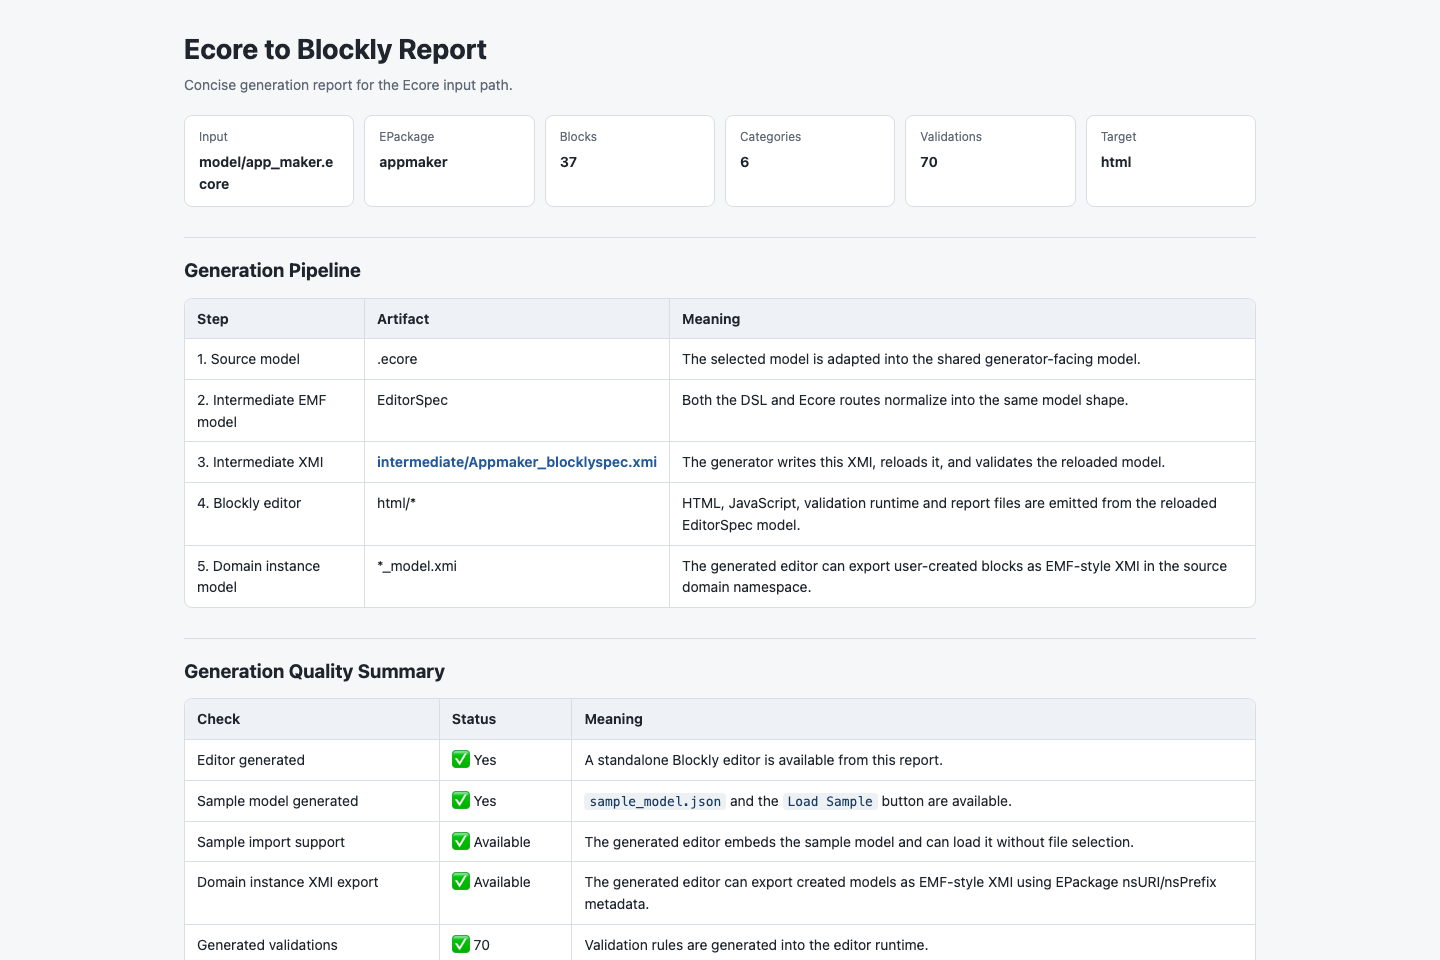
\includegraphics[width=0.90\textwidth,trim=150 300 150 30,clip]{assets/appmaker/appmaker-ecore-generation-report.png}
  \caption{Informe abierto después de generar el editor desde
  \texttt{app\_maker.ecore}}
  \label{fig:appmaker-ecore-generation-report}
\end{figure}

Conviene distinguir las dos ejecuciones implicadas. La primera se realiza en
Eclipse y transforma la descripción del dominio en artefactos web. La segunda se
realiza en el navegador al abrir la página autónoma
\texttt{*\_standalone.html}; en ella,
el usuario construye modelos del dominio mediante bloques, ejecuta las
validaciones generadas y exporta el resultado como JSON, XMI o código textual.
La Figura \ref{fig:appmaker-ecore-editor} muestra esta segunda ejecución con el
modelo de ejemplo cargado en el workspace.

\begin{figure}[htbp]
  \centering
  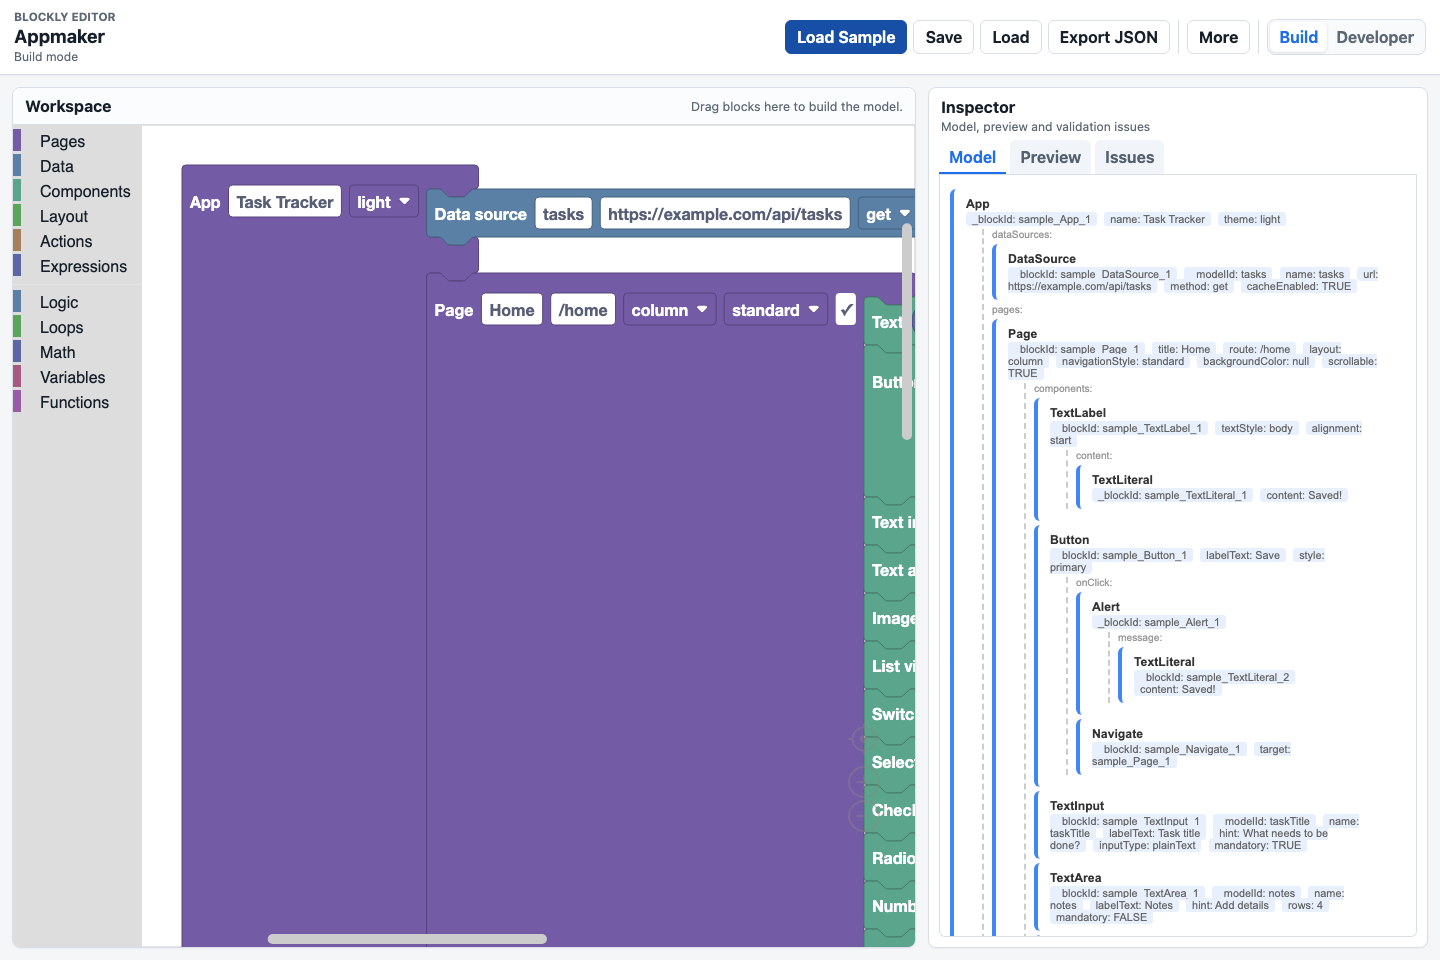
\includegraphics[width=\textwidth]{assets/appmaker/appmaker-ecore-editor.png}
  \caption{Editor Blockly ejecutado en el navegador después de la generación
  desde \texttt{app\_maker.ecore}}
  \label{fig:appmaker-ecore-editor}
\end{figure}

Las secciones siguientes abren esta cadena paso a paso y relacionan cada
operación visible con su implementación.

\section{Flujo interno de una ejecución}
\label{sec:flujo-interno-ejecucion}

En la ejecución integrada, la acción seleccionada por el usuario se atiende en
\texttt{GenerateBlocklyEditorHandler}. Esta clase determina la extensión del
fichero y elige una de las dos ramas de carga. La Figura
\ref{fig:flujo-interno-ejecucion} representa esta secuencia con los nombres de
los componentes implementados. No es una segunda arquitectura del sistema, sino
la traza concreta que sigue una petición de generación dentro del plugin.

\begin{figure}[htbp]
  \centering
  \resizebox{0.93\textwidth}{!}{%
  \begin{tikzpicture}[
      node distance=0.62cm and 1.15cm,
      box/.style={draw=black!55, rounded corners=2pt, minimum height=0.72cm,
        align=center, font=\small, inner sep=5pt},
      entrybox/.style={box, fill=black!5, text width=6.8cm},
      sourcebox/.style={box, fill=green!8, text width=4.1cm},
      routebox/.style={box, fill=blue!7, text width=4.1cm},
      commonbox/.style={box, fill=orange!10, text width=8.6cm},
      arrow/.style={-{Latex[length=2.4mm]}, thick, draw=black!70}
    ]
    \node[entrybox] (handler)
      {\texttt{GenerateBlocklyEditorHandler}\\selección de la ruta de entrada};

    \node[sourcebox, below left=of handler] (ecore)
      {Fichero \texttt{.ecore}};
    \node[sourcebox, below right=of handler] (dsl)
      {Fichero \texttt{.m2b}};

    \node[routebox, below=of ecore] (ecoreload)
      {\texttt{ResourceSet}\\+ \texttt{EPackage}};
    \node[routebox, below=of dsl] (dslload)
      {\texttt{XtextResource}\\+ \texttt{DomainModel}\\+ validación Xtext};

    \node[routebox, below=of ecoreload] (ecoreadapter)
      {\texttt{EcoreAdapter}\\implementado en Java};
    \node[routebox, below=of dslload] (dsladapter)
      {\texttt{DomainModelAdapter}\\implementado en Java};

    \path let \p1=(ecoreadapter), \p2=(dsladapter) in
      node[commonbox] (spec) at ($ (\p1)!0.5!(\p2) +(0,-1.35cm) $)
      {Modelo EMF común \texttt{EditorSpec}};
    \node[commonbox, below=of spec] (diagnostics)
      {\texttt{BlocklySpecDiagnostics}\\validación de la especificación común};
    \node[commonbox, below=of diagnostics] (xmi)
      {\texttt{BlocklySpecXmiSerializer}\\serialización, recarga y nueva validación};
    \node[commonbox, below=of xmi] (generator)
      {\texttt{BlocklyCodeGenerator} en Xtend\\generación modelo a texto};
    \node[commonbox, below=of generator] (output)
      {Directorio \texttt{\_generated}: informe, XMI intermedio,\\
       bloques, paleta, validaciones y páginas HTML};

    \draw[arrow] (handler) -- (ecore);
    \draw[arrow] (handler) -- (dsl);
    \draw[arrow] (ecore) -- (ecoreload);
    \draw[arrow] (dsl) -- (dslload);
    \draw[arrow] (ecoreload) -- (ecoreadapter);
    \draw[arrow] (dslload) -- (dsladapter);
    \draw[arrow] (ecoreadapter) -- (spec);
    \draw[arrow] (dsladapter) -- (spec);
    \draw[arrow] (spec) -- (diagnostics);
    \draw[arrow] (diagnostics) -- (xmi);
    \draw[arrow] (xmi) -- (generator);
    \draw[arrow] (generator) -- (output);
  \end{tikzpicture}%
  }
  \caption{Flujo interno implementado para una petición de generación}
  \label{fig:flujo-interno-ejecucion}
\end{figure}

En la rama Ecore, EMF carga el recurso y obtiene un \texttt{EPackage}; en la
rama textual, Xtext analiza, enlaza y valida el fichero antes de obtener un
\texttt{DomainModel}. Los adaptadores Java convierten ambos objetos en una
instancia de \texttt{EditorSpec}. A partir de ese punto, la ejecución es común:
se comprueba el modelo, se serializa como XMI, se vuelve a cargar y se valida de
nuevo antes de entregarlo al generador Xtend.

El generador devuelve un mapa de rutas y contenidos textuales. El manejador crea
el directorio de salida, escribe cada entrada del mapa y actualiza el workspace
de Eclipse. Esta última escritura explica por qué una única acción produce varios
ficheros relacionados y no solo la página autónoma mostrada en la sección
anterior. Las secciones posteriores detallan las operaciones resumidas en cada
caja de la figura.

\section{Organización del proyecto}
\label{sec:organizacion-proyecto}

La implementación se distribuye en tres bundles OSGi ejecutables creados según la
estructura habitual de Xtext \cite{xtextProject}. El proyecto
\path{io.github.plortinus.model2blockly} contiene la gramática, el modelo EMF
común, los adaptadores, la validación, los generadores y las entradas de línea de
comandos. El proyecto terminado en \path{.ide} aporta la configuración de los
servicios de lenguaje independientes de la interfaz. Finalmente, el proyecto
terminado en \path{.ui} registra el editor, los menús y los handlers que conectan
la generación con el workspace de Eclipse.

Otros dos proyectos no añaden lógica a la transformación. El proyecto
\path{.feature} agrupa los bundles instalables y \path{.updatesite} construye el
repositorio p2 utilizado para distribuir el plugin. Dentro de los tres bundles
ejecutables, la Tabla \ref{tab:paquetes-implementacion} relaciona cada componente
con los ficheros que materializan su implementación y con la tecnología empleada.

\begin{table}[H]
  \centering
  \small
  \setlength{\tabcolsep}{4pt}
  \begin{tabular}{@{}
      >{\raggedright\arraybackslash}p{0.17\textwidth}
      >{\raggedright\arraybackslash}p{0.40\textwidth}
      >{\raggedright\arraybackslash}p{0.32\textwidth}@{}}
    \toprule
    Componente & Implementación concreta & Función en la ejecución \\
    \midrule
    DSL textual & \texttt{Model2Blockly.xtext} (Xtext) y
    \texttt{Model2BlocklyValidator.java} (Java) & Analizar y validar una entrada
    \texttt{.m2b}. \\

    Modelo EMF común & \texttt{blockly\_editor\_spec.ecore} y código Java generado
    en \texttt{emf-gen} & Representar la especificación normalizada
    \texttt{EditorSpec}. \\

    Adaptadores & \texttt{EcoreAdapter.}\allowbreak\texttt{toEditorSpec}
    \allowbreak\texttt{(EPackage)} y
    \texttt{DomainModelAdapter.}\allowbreak\texttt{toEditorSpec}
    \allowbreak\texttt{(DomainModel)} (Java) & Recorrer cada
    modelo de entrada y construir el mismo \texttt{EditorSpec}. \\

    Diagnóstico y XMI & \texttt{BlocklySpecDiagnostics.java} y
    \texttt{BlocklySpecXmiSerializer.java} (Java) & Validar, serializar y volver a
    cargar el modelo común. \\

    Generación & \texttt{BlocklyCodeGenerator.xtend} (Xtend) y clases auxiliares
    del paquete \texttt{generator} (Java) & Producir HTML, JavaScript, JSON,
    informes y modelos de ejemplo. \\

    Integración Eclipse & \texttt{GenerateBlocklyEditor}\allowbreak
    \texttt{Handler.java} (Java) y \texttt{plugin.xml} & Registrar el comando,
    ejecutar la cadena y escribir sus resultados en el workspace. \\

    Ejecución standalone & Clases \texttt{*Main.java} del paquete
    \texttt{standalone} (Java) & Exponer la generación y el parcheado mediante
    línea de comandos. \\

    Pruebas & Clases \texttt{*Test.java} del directorio \texttt{test}
    (JUnit/Java) & Comprobar adaptadores, modelo común, validación y generación. \\
    \bottomrule
  \end{tabular}
  \caption{Organización de los componentes implementados}
  \label{tab:paquetes-implementacion}
\end{table}

En particular, la fila \emph{Adaptadores} corresponde a dos clases escritas
manualmente en Java, no a código de transformación generado por Xtext. Sus
métodos públicos reciben objetos EMF que ya han sido cargados: un
\texttt{EPackage} en la primera ruta y un \texttt{DomainModel} en la segunda.
Ambas clases recorren esos objetos mediante sus API tipadas y delegan la creación
final de la instancia EMF de \texttt{EditorSpec} en
\texttt{BlocklySpecModelMapper}. Las secciones
\ref{sec:implementacion-ecore-adapter} y
\ref{sec:implementacion-domainmodel-adapter} detallan las reglas aplicadas por
cada clase.

Esta organización materializa la arquitectura del capítulo anterior sin
repetirla: allí se justificaron los componentes y sus dependencias; aquí se
identifican las clases, los lenguajes y los artefactos que ejecutan esas
responsabilidades.

\section{Carga y validación de las entradas}
\label{sec:carga-validacion-entradas}

La carga se implementa antes de los adaptadores. \texttt{EcoreAdapter} recibe un
objeto EMF ya construido y \texttt{DomainModelAdapter} recibe el modelo tipado
producido por Xtext; ninguna de las dos clases abre ficheros. En la ejecución
desde Eclipse, esta responsabilidad reside en
\texttt{GenerateBlocklyEditorHandler}; las clases de entrada independiente reproducen el mismo
patrón para ficheros situados fuera del workspace. El resultado de esta etapa es
un \texttt{EPackage} o un \texttt{DomainModel} válido para iniciar la
transformación.

\subsection{Carga de un metamodelo \texttt{.ecore}}

El método \texttt{generateFromEcore} registra
\texttt{EcoreResourceFactoryImpl} para la extensión \texttt{ecore}, crea un
\texttt{ResourceSetImpl} y construye una URI de fichero a partir de la ubicación
del recurso seleccionado. La llamada \texttt{getResource(uri, true)} solicita la
carga inmediata del documento XMI y EMF resuelve sus elementos y referencias. El
primer objeto raíz se obtiene como \texttt{EPackage} y se entrega a
\texttt{EcoreAdapter}. La clase \texttt{EcoreToBlocklyMain} utiliza la misma
secuencia en su método \texttt{loadEPackage}.

Esta rama no utiliza el parser ni el validador de Xtext. Los problemas que
impiden leer el recurso se propagan como excepciones de carga; las restricciones
específicas que necesita el generador se comprueban después de la adaptación
mediante \texttt{BlocklySpecDiagnostics}. Esta separación evita interpretar
como sintaxis textual un metamodelo que ya dispone del formato estándar de EMF.

\subsection{Carga y validación de una entrada \texttt{.m2b}}

La ruta textual comienza registrando el lenguaje con
\texttt{Model2BlocklyStandalone}\allowbreak\texttt{Setup}. La configuración generada por Xtext
asocia el mismo lenguaje con las extensiones \texttt{.m2b} y
\texttt{.model2blockly}; la segunda se conserva por compatibilidad. El inyector
de Guice proporciona el \texttt{ResourceSet}, que carga el fichero como un
\texttt{XtextResource}. El parser crea el árbol EMF y el enlazador resuelve los
nombres usados para categorías, superclases y tipos. Si la carga termina
correctamente, el primer elemento del recurso debe ser una instancia de
\texttt{DomainModel}.

El Listado \ref{lst:carga-modelo-m2b} resume las llamadas Java que implementan
esta etapa en el manejador. La clase de entrada independiente
\texttt{Model2BlocklyToBlocklyMain} contiene la misma secuencia, cambiando
únicamente el origen de la ruta del fichero.

\begin{lstlisting}[language=Java, caption={Secuencia esencial de carga y validación de una entrada \texttt{.m2b}}, label={lst:carga-modelo-m2b}]
Injector injector = new Model2BlocklyStandaloneSetup()
    .createInjectorAndDoEMFRegistration();
ResourceSet resourceSet = injector.getInstance(ResourceSet.class);
Resource resource = resourceSet.getResource(fileUri, true);
XtextResource xtext = (XtextResource) resource;

xtext.validateConcreteSyntax();
Model2BlocklyValidationDiagnostics.throwIfSyntaxErrors(
    sourceLabel, resource.getErrors());
Model2BlocklyValidationDiagnostics.throwIfErrors(
    sourceLabel,
    xtext.getResourceServiceProvider().getResourceValidator()
        .validate(resource, CheckMode.ALL,
            CancelIndicator.NullImpl));

DomainModel domain =
    (DomainModel) resource.getAllContents().next();
\end{lstlisting}

La primera comprobación recoge los errores producidos durante el análisis y el
enlazado. A continuación, el \texttt{IResourceValidator} ejecuta en modo
\texttt{ALL} las reglas \texttt{@Check} de
\texttt{Model2BlocklyValidator}. Estas reglas detectan, entre otros casos,
nombres de clase duplicados, cardinalidades incoherentes, entradas de valor con
un tipo no válido, widgets incompatibles, referencias a campos inexistentes y
expresiones de validación no soportadas. El método \texttt{throwIfErrors} detiene
la generación únicamente ante diagnósticos de severidad \emph{error}; las
advertencias permanecen visibles en el editor, pero permiten continuar.

\subsection{Niveles de validación y comunicación de errores}

La implementación aplica tres niveles consecutivos. Primero se comprueba que el
recurso pueda cargarse y, en la ruta textual, que su sintaxis y sus referencias
sean correctas. Después se ejecutan las reglas semánticas específicas del DSL.
Finalmente, tras llamar al adaptador correspondiente,
\texttt{BlocklySpecDiagnostics.assertValid} comprueba las invariantes del
\texttt{EditorSpec} común. Esta última validación se repite después de serializar
y recargar el XMI, por lo que el generador solo recibe un modelo que ha superado
el contrato intermedio completo.

Cuando la ejecución se realiza en Eclipse, los errores semánticos y los
diagnósticos del modelo común se convierten en marcadores
\texttt{IMarker.PROBLEM} asociados al fichero y, cuando existe información de
origen, a su línea. El manejador vuelve a abrir la entrada y muestra un diálogo con
el resumen. En las entradas independientes, el mismo diagnóstico se escribe en la
salida de error y el proceso termina con un código distinto de cero. De este
modo, las dos formas de ejecución comparten las comprobaciones, aunque presentan
el resultado mediante interfaces diferentes.

\section{Ruta textual \texttt{.m2b} con Xtext}
\label{sec:implementacion-xtext}

La gramática Xtext define el lenguaje textual de entrada \texttt{.m2b} y
vincula sus reglas con los conceptos del metamodelo EMF asociado. A partir de
esta gramática, Xtext genera el parser y el soporte de edición
\cite{xtextProject,bettini2013xtext,bettini2015xsemantics}. Así, cada fichero
DSL puede tratarse como un modelo EMF. La raíz de ese modelo agrupa el nombre
del dominio, las opciones de generación, la configuración del workspace, las
categorías, las clases y las restricciones.

Las clases del dominio se declaran con una construcción específica del DSL. Cada
clase puede ser abstracta, generar un bloque de salida, heredar de otra clase,
pertenecer a una categoría, definir color, etiqueta, tooltip, disposición en
línea y plantilla de código. Dentro de una clase se declaran cuatro tipos de
elementos: atributos, contenciones, referencias y entradas de valor. Esta
distinción en la gramática se corresponde con las formas principales en las que
Blockly representa información: campos, entradas de sentencias, desplegables de
referencia y conectores de valor.

El DSL también incluye opciones de interfaz. Con estas opciones se pueden indicar
widgets, etiquetas, textos de ayuda, grupos,
orden de presentación, campos de solo lectura, campos ocultos y campos usados
para mostrar referencias. Esta información no es necesaria para un editor
Blockly básico, pero permite enriquecer la salida generada sin escribir
JavaScript a mano. En la memoria se usa para explicar la correspondencia con
Ecore y para mostrar una forma más compacta de definir el mismo lenguaje
AppMaker.

El Listado \ref{lst:appmaker-dsl} muestra un fragmento representativo de la
ruta textual \texttt{.m2b} aplicado al dominio AppMaker. En pocas líneas se
declaran una categoría, un bloque raíz, una contención con cardinalidad y un
bloque que referencia dinámicamente una fuente de datos. La misma información
acabaría convertida en campos, entradas y validaciones dentro del modelo
intermedio.

\begin{lstlisting}[caption={Fragmento representativo del DSL textual \texttt{.m2b} para AppMaker}, label={lst:appmaker-dsl}]
domain Appmaker codeLanguage "javascript" codeFileExtension "js"

category Pages label "Pages" colour 260
category Components label "Components" colour 160
category Data label "Data" colour 210

class App category Pages colour 260 label "App" {
  attribute name : string default "Task Tracker" required
    widget text uiLabel "App name" group "App" order 1
  contains DataSource dataSources [1..20]
    uiLabel "Data sources" group "Data" order 3
  contains Page pages [1..20]
    uiLabel "Pages" group "Pages" order 4
}

class ListView extends Component category Components colour 160 label "List view" {
  reference DataSource source required
    widget reference-select uiLabel "Source" referenceLabelField name
  value TextExpression itemTitle shadow TextLiteral
}
\end{lstlisting}

Una vez analizado el fichero como se explicó en la Sección
\ref{sec:carga-validacion-entradas}, el resultado de esta gramática es un
\texttt{DomainModel} enlazado y validado. Ese objeto constituye la entrada del
adaptador Java descrito posteriormente en la Sección
\ref{sec:implementacion-domainmodel-adapter}.

\section{Modelo intermedio EMF y vista Java}
\label{sec:implementacion-modelo-intermedio}

El contrato del modelo intermedio está definido como metamodelo EMF en el
fichero \texttt{blockly\_editor\_spec.ecore}, dentro del directorio
\texttt{model}. EMF genera a partir de él las interfaces Java
\texttt{EditorSpec}, \texttt{BlockTypeSpec}, \texttt{FieldSpec} y los demás
tipos del paquete \texttt{intermediate.blocklyspec}, junto con
\texttt{BlocklySpecFactory}. Para facilitar la construcción de esas instancias,
el proyecto conserva además \texttt{BlocklyEditorSpec}, una vista Java auxiliar del
mismo contenido. \texttt{BlocklySpecModelMapper} implementa la copia en ambos
sentidos entre esa vista y las instancias creadas por la factoría EMF.

El objeto EMF no se entrega directamente al generador después de la adaptación.
La serialización se encapsula en
\texttt{BlocklySpecXmi}\allowbreak\texttt{Serializer}. Esta clase crea un
\texttt{ResourceSet}\allowbreak\texttt{Impl} y registra
\texttt{BlocklySpecPackage.}\allowbreak\texttt{eNS\_URI} y añade el
\texttt{EditorSpec} a un \texttt{XMIResource}\allowbreak\texttt{Impl} con la
URI en memoria \texttt{memory:/}\allowbreak\texttt{blocklyspec.xmi}. El recurso se guarda en UTF-8, se vuelve a
cargar desde esa cadena y se comprueba que su raíz siga siendo un
\texttt{EditorSpec}. El Listado \ref{lst:ciclo-editor-spec-xmi} muestra cómo el
manejador aplica este ciclo en las dos rutas de entrada.

\begin{lstlisting}[language=Java, caption={Validación, serialización y recarga del modelo intermedio}, label={lst:ciclo-editor-spec-xmi}]
BlocklySpecDiagnostics.assertValid(intermediateModel, sourceLabel,
    sourceMapper);

String intermediateXmi =
    BlocklySpecXmiSerializer.toXmi(intermediateModel);
EditorSpec spec =
    BlocklySpecXmiSerializer.fromXmiToEditorSpec(intermediateXmi);

BlocklySpecDiagnostics.assertValid(
    spec, sourceLabel + " intermediate XMI");
Map<String, String> generated =
    new BlocklyCodeGenerator().generate(spec);
\end{lstlisting}

En el extracto, \texttt{sourceMapper} representa el mapeador creado por
\texttt{forEPackage} o \texttt{forDomainModel}, según la ruta. El primer
diagnóstico puede asociarse con elementos del modelo fuente mediante
\texttt{sourceMapper}; el segundo valida el objeto recargado. De este modo, un
error de serialización, una raíz incorrecta o la pérdida de un dato obligatorio
se detectan antes de generar texto. La misma cadena XMI se conserva después como
\path{intermediate/*_blocklyspec.xmi}, por lo que el artefacto inspeccionable es
exactamente el contenido usado para generar el editor.

Cada tipo de bloque guarda su forma de conexión: bloque raíz, bloque apilable,
bloque apilable tipado, bloque de valor o bloque de valor tipado. Esta
clasificación permite generar las conexiones visuales adecuadas sin mezclar
reglas específicas de Blockly con la lectura del dominio. La implementación
mantiene además listas separadas para campos, entradas de sentencias,
referencias y entradas de valor, lo que facilita generar cada tipo de elemento
con la construcción Blockly adecuada.

El modelo intermedio también conserva información de orden para las entradas de
un bloque. Esta decisión es relevante para la ruta Ecore: cuando las
características de una clase se leen desde el metamodelo, el orden
original de atributos y referencias puede influir en la legibilidad del bloque
generado. El generador usa esta lista cuando está disponible y, si no existe,
aplica un orden por defecto.

La ventaja de esta implementación es el desacoplamiento. Los adaptadores de
entrada producen una instancia conforme al mismo metamodelo intermedio, y los
generadores consumen su vista Java sin depender de cómo fue creada. Así, las
entradas y las salidas quedan separadas en el código, pero el contrato MDE sigue
siendo el metamodelo EMF y su serialización XMI.

\section{Adaptador desde Ecore}
\label{sec:implementacion-ecore-adapter}

Los dos adaptadores se implementan como clases Java ordinarias con métodos
estáticos; no se instancian ni contienen plantillas de generación. El Listado
\ref{lst:entrada-adaptadores-java} muestra sus puntos de entrada reales. Cada
método realiza primero una normalización hacia \texttt{BlocklyEditorSpec}, una
vista Java interna formada por listas y objetos tipados, y después invoca
\texttt{BlocklySpecModelMapper.toEmfSpec}. Este segundo paso usa
\texttt{BlocklySpecFactory.eINSTANCE} para crear el \texttt{EditorSpec} definido
por el metamodelo común y copiar recursivamente categorías, bloques, campos,
entradas, validaciones y opciones de workspace. Por tanto, la vista Java es un
objeto auxiliar de construcción; el resultado contractual del adaptador es la
instancia EMF \texttt{EditorSpec}.

\begin{lstlisting}[float=htbp, language=Java, caption={Puntos de entrada Java de los dos adaptadores}, label={lst:entrada-adaptadores-java}]
// EcoreAdapter.java
public static EditorSpec toEditorSpec(EPackage pkg) {
    return BlocklySpecModelMapper.toEmfSpec(fromEPackage(pkg));
}

// DomainModelAdapter.java
public static EditorSpec toEditorSpec(DomainModel domain) {
    return BlocklySpecModelMapper.toEmfSpec(fromDomainModel(domain));
}
\end{lstlisting}

En la ruta Ecore, \texttt{fromEPackage} recibe el objeto obtenido durante la
carga descrita en la Sección \ref{sec:carga-validacion-entradas}. El método copia
primero el nombre, \texttt{nsURI}, prefijo y opciones globales del paquete.
Después reúne los nombres de las clases que son destino de alguna referencia de
contención; este conjunto se usa más adelante para distinguir bloques raíz de
bloques que deben conectarse como hijos. A continuación recorre todos los
\texttt{EClassifier} del paquete y de sus subpaquetes, selecciona los
\texttt{EClass} y llama a \texttt{convertEClass}. Este proceso usa directamente
la API de EMF: clases, atributos, referencias, herencia y cardinalidades
\cite{emfOverview}.

Desde el punto de vista de MDE, este adaptador es una transformación de modelos
implementada en Java sobre la API de EMF. No se ha usado un lenguaje específico
de transformación como ATL o ETL. La razón es pragmática: el generador debe
integrarse dentro de un plugin Eclipse/Xtext, reutilizar utilidades Java del
proyecto, emitir diagnósticos concretos sobre el fichero de entrada y construir
la instancia EMF \texttt{EditorSpec} que después se serializa como XMI. La
implementación queda así dentro de la misma cadena Java que carga el recurso y
comunica los errores al entorno Eclipse. La Tabla
\ref{tab:transformacion-ecore-editor-spec} resume las reglas principales de la
transformación.

El mapeo estructural se implementa de forma automática. Un atributo Ecore se
transforma en un campo visual; su tipo determina si el campo Blockly será
textual, numérico, booleano, desplegable, color, ángulo o imagen. Una referencia
de contención se transforma en una entrada estructural, porque representa una
relación jerárquica entre elementos del modelo. Una referencia no contenida se
transforma en una referencia dinámica, porque apunta a otro elemento ya
existente. Las cardinalidades se convierten en reglas de validación para que el
editor generado pueda avisar al usuario si faltan elementos obligatorios, si se
supera un límite superior o si un campo requerido queda sin completar.

La inferencia de conexiones también se realiza en el adaptador. Las clases
contenedoras que no están contenidas por otras pueden convertirse en bloques
raíz sin conexión vertical. Las clases que heredan de una superclase pueden
generar conexiones tipadas. Las clases marcadas como bloques de salida generan
conectores de valor. Esta inferencia es importante porque evita que el usuario
tenga que escribir a mano reglas de conexión Blockly para cada clase.

\begin{table}[H]
  \centering
  \small
  \begin{tabular}{|L{0.30\textwidth}|L{0.30\textwidth}|L{0.26\textwidth}|}
    \hline
    Elemento Ecore de entrada & Elemento \texttt{EditorSpec} destino & Uso en Blockly \\
    \hline
    \texttt{EPackage} & \texttt{EditorSpec} con nombre, \texttt{nsURI} y opciones
    globales & Identidad del editor y exportación XMI. \\
    \texttt{EClass} concreta & \texttt{BlockTypeSpec} & Tipo de bloque disponible en
    la paleta. \\
    \texttt{EClass} abstracta & \texttt{BlockTypeSpec} abstracto & Tipo usado para
    conexiones, pero no instanciable. \\
    \texttt{EAttribute} & \texttt{FieldSpec} & Campo de texto, número, booleano,
    color, ángulo o desplegable. \\
    \texttt{EReference containment=true} & \texttt{StatementInputSpec} & Entrada
    vertical para bloques hijos. \\
    \texttt{EReference containment=false} & \texttt{ReferenceFieldSpec} & Desplegable
    dinámico hacia elementos existentes. \\
    \texttt{lowerBound}/\texttt{upperBound} & \texttt{ValidationSpec} y límites de
    entrada & Avisos de obligatoriedad y cardinalidad. \\
    \texttt{EAnnotation} & Metadatos de bloque, interfaz, validación o código &
    Color, categoría, etiqueta, tooltip, widget y plantilla. \\
    \hline
  \end{tabular}
  \caption{Transformación principal de Ecore a \texttt{EditorSpec}}
  \label{tab:transformacion-ecore-editor-spec}
\end{table}

El adaptador permite enriquecer la generación mediante anotaciones Ecore. Las
anotaciones con fuente \texttt{blockly} afectan a la sintaxis visual: etiqueta,
color, categoría, tooltip, disposición en línea, bloque de salida, rangos
numéricos, entradas de valor o shadow blocks. Las anotaciones con fuente
\texttt{ui} se incorporan al modelo intermedio para personalizar la salida HTML. Las
anotaciones con fuente \texttt{code} permiten definir lenguaje, extensión de
archivo y plantillas de generación. Así, un metamodelo sin anotaciones puede
generar un editor básico, mientras que un metamodelo anotado puede producir una
experiencia más adaptada al dominio.

El Listado \ref{lst:appmaker-ecore} muestra el mismo tipo de información en la
ruta Ecore. El metamodelo conserva las clases y referencias EMF, y las
anotaciones añaden la sintaxis visual, la regla de validación y la plantilla de
código usadas por el generador.

\begin{lstlisting}[caption={Fragmento de \texttt{model/app\_maker.ecore} con anotaciones}, label={lst:appmaker-ecore}]
<eClassifiers xsi:type="ecore:EClass" name="Navigate" eSuperTypes="#//Action">
  <eAnnotations source="blockly">
    <details key="colour" value="30"/>
    <details key="category" value="Actions"/>
    <details key="inputsInline" value="true"/>
  </eAnnotations>
  <eAnnotations source="validation">
    <details key="mustFollow" value="Alert"/>
  </eAnnotations>
  <eAnnotations source="code">
    <details key="template" value="navigate(&quot;{{target}}&quot;);"/>
  </eAnnotations>
  <eStructuralFeatures xsi:type="ecore:EReference" name="target"
      lowerBound="1" eType="#//Page">
    <eAnnotations source="ui">
      <details key="widget" value="reference-select"/>
      <details key="label" value="Target page"/>
      <details key="referenceLabelField" value="title"/>
    </eAnnotations>
  </eStructuralFeatures>
</eClassifiers>
\end{lstlisting}

\section{Adaptador desde la ruta textual \texttt{.m2b}}
\label{sec:implementacion-domainmodel-adapter}

El adaptador de la ruta textual también está implementado manualmente en Java.
\texttt{DomainModelAdapter.fromDomainModel} recibe la raíz EMF producida por
Xtext y ejecuta, en orden, los métodos \texttt{convertCategories},
\texttt{convertClasses}, \texttt{convertConstraints},
\texttt{convertValidations} y \texttt{convertWorkspaceOptions}. Después genera
las validaciones inferidas de cardinalidad, obligatoriedad y unicidad. El objeto
Java resultante vuelve al método \texttt{toEditorSpec} del Listado
\ref{lst:entrada-adaptadores-java}, donde se convierte al mismo modelo EMF común
que en la ruta Ecore.

El mapeo es más directo que en Ecore porque la gramática ya distingue los
conceptos específicos que necesita Model2Blockly. Los atributos se convierten en
campos, las contenciones en entradas estructurales, las referencias en
desplegables dinámicos y las entradas de valor en conexiones horizontales. Las
restricciones de orden se convierten en validaciones, y los campos marcados como
obligatorios generan comprobaciones de obligatoriedad.

La conversión de cada clase se implementa con un recorrido de la lista
\texttt{Feature} generada por Xtext. El Listado
\ref{lst:despacho-domainmodel-adapter} muestra el despacho esencial. Cada tipo
concreto se entrega a un método especializado y el nombre de la entrada se añade
a \texttt{orderedInputNames}; de este modo, el orden escrito en el fichero
\texttt{.m2b} se conserva al construir el bloque.

\begin{lstlisting}[language=Java, caption={Despacho de elementos del DSL en \texttt{DomainModelAdapter}}, label={lst:despacho-domainmodel-adapter}]
for (Feature feature : cls.getFeatures()) {
    if (feature instanceof Attribute) {
        FieldSpec field = convertAttribute((Attribute) feature);
        bt.getFields().add(field);
        bt.getOrderedInputNames().add(field.getName());
    } else if (feature instanceof Containment) {
        StatementInputSpec input =
            convertContainment((Containment) feature);
        bt.getStatementInputs().add(input);
        bt.getOrderedInputNames().add(input.getName());
    } else if (feature instanceof Reference) {
        ReferenceFieldSpec reference =
            convertReference((Reference) feature);
        bt.getReferenceFields().add(reference);
        bt.getOrderedInputNames().add(reference.getName());
    } else if (feature instanceof ValueInput) {
        ValueInputSpec input = convertValueInput((ValueInput) feature);
        bt.getValueInputs().add(input);
        bt.getOrderedInputNames().add(input.getName());
    }
}
\end{lstlisting}

\begin{table}[htbp]
  \centering
  \small
  \begin{tabular}{|L{0.30\textwidth}|L{0.30\textwidth}|L{0.26\textwidth}|}
    \hline
    Elemento del DSL & Elemento \texttt{EditorSpec} destino & Uso en Blockly \\
    \hline
    \texttt{domain} & \texttt{EditorSpec} & Nombre del editor y opciones de
    generación. \\
    \texttt{category} & \texttt{CategorySpec} & Categoría de la paleta y color por
    defecto. \\
    \texttt{class} & \texttt{BlockTypeSpec} & Tipo de bloque. \\
    \texttt{attribute} & \texttt{FieldSpec} & Campo visual del bloque. \\
    \texttt{contains [m..n]} & \texttt{StatementInputSpec} y
    \texttt{ValidationSpec} & Entrada de hijos y comprobación de cardinalidad. \\
    \texttt{reference} & \texttt{ReferenceFieldSpec} & Desplegable dinámico. \\
    \texttt{value} & \texttt{ValueInputSpec} & Entrada horizontal para bloques de
    valor. \\
    \texttt{must follow} & \texttt{ValidationSpec} & Regla local de orden. \\
    \hline
  \end{tabular}
  \caption{Normalización del DSL textual \texttt{.m2b} a \texttt{EditorSpec}}
  \label{tab:transformacion-dsl-editor-spec}
\end{table}

La implementación usa también información de herencia para determinar la forma
de conexión. Una clase marcada como bloque de salida se convierte en bloque de
valor; una clase con superclase genera conexiones tipadas; una clase con
contenciones y sin superclase puede funcionar como bloque raíz; y una clase
ordinaria se genera como bloque apilable. De este modo, la semántica declarada
en la sintaxis textual se transforma en reglas visuales de Blockly sin que el
autor del dominio tenga que conocer la API de bajo nivel de la biblioteca.

La estructura principal se lee con los tipos Java generados por Xtext
(\texttt{ClassDef}, \texttt{Attribute}, \texttt{Containment},
\texttt{Reference} y \texttt{ValueInput}). Solo algunas opciones de interfaz,
código y workspace se obtienen dinámicamente con
\texttt{eClass().getEStructuralFeature} y \texttt{eGet}. Esta decisión permite
que metadatos añadidos recientemente a la gramática puedan leerse antes de
regenerar todos los accesores, sin renunciar a la comprobación estática en el
recorrido estructural que determina los bloques.

\section{Generador HTML/JavaScript}
\label{sec:implementacion-generador-html}

El generador de la salida HTML/JavaScript transforma el modelo intermedio en los
artefactos necesarios para abrir el editor en un navegador: bloques, paleta,
exportación, validaciones, página de edición, página autónoma, workspace de
validaciones, modelo de ejemplo e informe de generación. Esta salida usa Blockly
para definir bloques, inyectar el workspace, gestionar la paleta, serializar y
generar código \cite{blocklyDocs}.

La generación de código se implementa principalmente en Xtend. La clase
principal, \texttt{Blockly\allowbreak{}Code\allowbreak{}Generator.xtend}, recibe
un \texttt{EditorSpec} y produce un mapa ordenado de nombres de fichero a
contenido textual. El Listado \ref{lst:entrada-generador-xtend} reproduce el
método de entrada: cada función \texttt{generate*} devuelve una cadena y el mapa
conserva la relación entre esa cadena y su fichero de destino.

\begin{lstlisting}[captionpos=t, caption={Método de entrada de \texttt{BlocklyCodeGenerator.xtend}}, label={lst:entrada-generador-xtend}]
def Map<String, String> generate(EditorSpec spec) {
    val files = new LinkedHashMap<String, String>()
    val base = spec.domainName ?: "domain"
    files.put(base + "_blocks.js", generateBlocksJs(spec))
    files.put(base + "_toolbox.js", generateToolboxJs(spec))
    files.put(base + "_generators.js", generateGeneratorsJs(spec))
    files.put(base + "_validations.js", generateValidationsJs(spec))
    files.put(base + "_editor.html", generateEditorHtml(spec))
    files.put(base + "_standalone.html", generateStandaloneHtml(spec))
    files.put("validation_workspace.html",
        ValidationWorkspaceHtmlGenerator.generate(spec))
    files.put("validation_blocks.json",
        ValidationBlockModelGenerator.generate(spec))
    files.put("validation_runtime.js",
        ValidationRuntimeGenerator.generateClassicJs(spec))
    files.put("sample_model.json", SampleModelGenerator.generate(spec))
    return files
}
\end{lstlisting}

Xtend se usa como mecanismo de generación porque se integra bien con Xtext y
permite escribir plantillas de
texto legibles dentro del proyecto Eclipse. No se ha usado Acceleo ni un motor
externo de plantillas. Algunas piezas auxiliares, como el modelo de ejemplo, el
runtime de validaciones y la vista visual de reglas, se implementan en clases
Java separadas para mantener responsabilidades acotadas.

El mapa no escribe directamente en disco. El
\texttt{GenerateBlocklyEditorHandler} antepone \texttt{html/} a sus rutas y
añade tres resultados producidos fuera de Xtend: el XMI intermedio, el
\texttt{README.md} y el informe de generación. Finalmente,
\texttt{writeFiles} crea los \texttt{IFile} del workspace y actualiza el proyecto.
Esta separación permite reutilizar el mismo generador desde las entradas
standalone sin depender de la API de Eclipse.

La generación de bloques comienza en \texttt{generateBlocksArray}, que filtra
los tipos concretos y llama a \texttt{blockTypeToBlockJson}. Este método crea
mapas de campos, referencias y entradas, y recorre
\texttt{orderedInputNames} para conservar el orden establecido por el
adaptador. Cada elemento se delega en \texttt{fieldToArg},
\texttt{referenceToArg}, \texttt{valueInputToArg} o
\texttt{statementInput}\allowbreak\texttt{ToArg}. Finalmente, un
\texttt{switch} sobre \texttt{Connection}\allowbreak\texttt{Type} emite
\texttt{previous}\allowbreak\texttt{Statement},
\texttt{nextStatement} u \texttt{output} con tipo libre o tipado. Las clases
abstractas quedan en el modelo para resolver herencia y conexiones, pero no se
incluyen como bloques instanciables.

La generación de la paleta produce el conjunto de bloques disponible para el
usuario. Si no hay categorías, el generador puede emitir una paleta simple. Si
existen categorías, genera una paleta categorizada, incluyendo subcategorías cuando se
han definido. También se incluyen categorías integradas de Blockly, como lógica,
bucles, matemáticas, variables y funciones, para que los dominios puedan
combinar bloques propios con construcciones generales cuando sea necesario.

Se generan dos envoltorios HTML sobre esos mismos contenidos. La página
\texttt{*\_editor.}\allowbreak\texttt{html} carga por separado los ficheros de bloques, paleta,
generadores y validaciones, lo que facilita incrustarla y depurar cada módulo.
La página \texttt{*\_standalone.html} incrusta el JavaScript específico del
dominio en un único documento para simplificar la demostración. En ambos casos,
la biblioteca Blockly y su generador JavaScript se cargan desde la CDN indicada
en las etiquetas \texttt{script}; por ello, la página autónoma no contiene una
copia local de Blockly y requiere acceso a esa dependencia al abrirse.

La Tabla \ref{tab:artefactos-generados} resume los ficheros principales que
emite la cadena generativa. Esta lista permite interpretar la salida como un
resultado reproducible y no como una única página HTML aislada.

\begin{table}[htbp]
  \centering
  \small
  \begin{tabular}{|L{0.32\textwidth}|L{0.54\textwidth}|}
    \hline
    Artefacto generado & Contenido \\
    \hline
    \texttt{html/*\_blocks.js} & Definiciones de bloques Blockly. \\
    \texttt{html/*\_toolbox.js} & Categorías y paleta del editor. \\
    \texttt{html/*\_generators.js} & Funciones de serialización y generación de
    código por bloque. \\
    \texttt{html/*\_validations.js} & Reglas de validación ejecutadas sobre el
    workspace. \\
    \texttt{html/*\_editor.html} & Página embebible del editor generado. \\
    \texttt{html/*\_standalone.html} & Página única que incrusta el código del
    dominio y carga Blockly desde CDN. \\
    \texttt{html/sample\_model.json} & Modelo de ejemplo usado por el botón
    \texttt{Load Sample}. \\
    \path{html/validation_workspace.html} & Editor visual de reglas de
    validación. \\
    \path{html/validation_blocks.json} & Árbol serializado de bloques de
    validación. \\
    \path{html/validation_runtime.js} & Compilación y evaluación de las reglas
    visuales en el navegador. \\
    \path{intermediate/*_blocklyspec.xmi} & Instancia XMI de
    \texttt{EditorSpec} recargada antes de generar HTML. \\
    \texttt{generation\_report.html} & Informe de trazabilidad de la generación. \\
    \texttt{README.md} & Instrucciones para abrir y revisar los resultados. \\
    \hline
  \end{tabular}
  \caption{Artefactos principales emitidos por la cadena generativa}
  \label{tab:artefactos-generados}
\end{table}

Entre esos artefactos, la exportación tiene dos objetivos. Por un lado,
serializa el workspace como una estructura JSON con el tipo de bloque,
identificador, campos, referencias, valores y sentencias. También puede exportar
ese contenido como XMI de instancia del dominio, usando el prefijo y el URI del
paquete de entrada y evitando mezclar ese XMI con el XMI intermedio
\texttt{EditorSpec}. Por otro lado, incorpora una ruta de generación de código
basada en plantillas. Si un bloque define una plantilla, el generador sustituye
marcadores por valores de campos, entradas de valor o secuencias de sentencias.
Si no existe plantilla, se usa una representación textual genérica. Esta
estrategia mantiene la exportación operativa incluso cuando el dominio todavía
no ha definido una semántica de código completa.

\section{Validaciones y referencias en tiempo de ejecución}
\label{sec:implementacion-validaciones-referencias}

La implementación distingue entre validación estática del DSL y validación en
tiempo de ejecución del editor generado. La primera se realiza en Eclipse/Xtext
antes de generar. La segunda se ejecuta en el navegador sobre el workspace
Blockly.

\texttt{generateValidationsJs} produce las funciones
\texttt{computeValidation}\allowbreak\texttt{Warnings},
\texttt{applyValidation}\allowbreak\texttt{Warnings} e
\texttt{init}\allowbreak\texttt{Validations}. La primera recorre
\texttt{workspace.}\allowbreak\texttt{getAllBlocks(false)} y evalúa las reglas aplicables a cada
tipo. Las reglas de orden consultan \texttt{getPreviousBlock}; las de
cardinalidad siguen la cadena iniciada en \texttt{getInputTargetBlock}; y las de
obligatoriedad y unicidad leen y comparan los valores de campo. La segunda
función agrupa los mensajes por bloque, llama a \texttt{setWarningText} y
actualiza el panel de problemas. \texttt{init}\allowbreak\texttt{Validations} registra finalmente un
listener para repetir el cálculo después de crear, borrar, mover o modificar un
bloque.

Las reglas se representan también como árboles en
\texttt{validation\_blocks.json}. La clase Java
\texttt{ValidationRuntimeGenerator} transforma cada árbol en una expresión de
runtime y genera \texttt{validation\_runtime.js}. En el navegador,
\texttt{createValidationAccessors} ofrece operaciones acotadas como
\texttt{value}, \texttt{has}, \texttt{inputCount}, \texttt{fieldUnique} y
\texttt{previousBlockIs}; \texttt{evaluateRuntimeExpression} ejecuta la
expresión con esos accesores. Esta representación permite que
\texttt{validation\_workspace.html} muestre las mismas reglas que utiliza el
editor, en lugar de mantener una segunda definición visual independiente.

Las referencias no contenidas se implementan como campos cuyos valores son
identificadores de bloques. La función generada
\texttt{updateReferenceDropdowns} agrupa las instancias existentes por tipo,
construye para cada destino una pareja etiqueta--identificador y sustituye las
opciones del desplegable. La etiqueta se toma del
\texttt{referenceLabelField}, del campo \texttt{name} o, como último recurso,
del tipo y una parte del identificador. Si se elimina el bloque referenciado, el
valor deja de estar entre las opciones válidas y se limpia.

Esta implementación mantiene la diferencia entre contención y referencia. Una
contención crea estructura jerárquica en el workspace, mientras que una
referencia selecciona un elemento que ya existe. La separación conserva la
información relacional del modelo de dominio.

Cuando existe una referencia opuesta, \texttt{synchronizeOppositeReferences}
calcula los valores inversos y actualiza el bloque destino. Una bandera
\texttt{\_\_syncingOpposite}\allowbreak\texttt{References} y la desactivación temporal de eventos
evitan que esa escritura genere un ciclo de notificaciones. El Listado
\ref{lst:listener-runtime-blockly} resume el listener compartido que mantiene
referencias, validaciones y vista de salida después de cada cambio estructural.

\begin{lstlisting}[caption={Actualización reactiva del editor generado}, label={lst:listener-runtime-blockly}]
workspace.addChangeListener(function(event) {
    if (event.type === Blockly.Events.BLOCK_MOVE ||
        event.type === Blockly.Events.BLOCK_CREATE ||
        event.type === Blockly.Events.BLOCK_DELETE ||
        event.type === Blockly.Events.BLOCK_CHANGE) {
        updateReferenceDropdowns(workspace);
        synchronizeOppositeReferences(workspace, event);
        if (typeof applyValidationWarnings === 'function')
            applyValidationWarnings(workspace);
        if (typeof updateOutput === 'function') updateOutput();
    }
});
\end{lstlisting}

Antes de exportar JSON, XMI o código, \texttt{confirmExportIfInvalid} vuelve a
ejecutar las validaciones y solicita confirmación si quedan advertencias. El
usuario puede por tanto inspeccionar un modelo incompleto sin bloquear la
edición, pero la exportación no oculta sus problemas. Los límites numéricos
\texttt{min} y \texttt{max} se incorporan directamente a los campos Blockly.

La página incluye además un ejecutor genérico de inspección.

El método \texttt{generateRuntimeScript} genera su código a partir del modelo.
Durante la ejecución, este código convierte el workspace a la
representación JSON del dominio, recorre recursivamente sus nodos y resalta el bloque visitado
con controles de ejecución, pausa y paso. No ejecuta la semántica particular de
cada dominio; sirve para observar la estructura construida y comprobar el orden
de recorrido del modelo.

El ciclo de validación se completa con una utilidad de parche. Desde línea de
comandos puede ejecutarse sobre un fichero
\texttt{validation\_blocks.edited.json} y desde Eclipse está expuesta como
\texttt{Apply Validation Blocks to Source}. El parche se aplica de forma
conservadora: solo actualiza reglas que se pueden mapear de manera inequívoca a
la sintaxis textual o a anotaciones Ecore, y deja fuera expresiones que no tengan
una traducción directa.

El comportamiento generado sigue siendo deliberadamente ligero. No constituye
un motor OCL completo ni un verificador semántico general. Cubre cardinalidad,
obligatoriedad, unicidad, referencias opuestas, expresiones declaradas y el
subconjunto de invariantes OCL que los adaptadores pueden traducir a los
accesores disponibles en JavaScript.

\section{Integración con Eclipse y distribución}
\label{sec:implementacion-eclipse-distribucion}

La integración con Eclipse se declara en el fichero \texttt{plugin.xml} del
bundle de interfaz. Este fichero registra los comandos
\texttt{generateBlocklyEditor} y \texttt{applyValidationPatch}, los asocia con
\texttt{GenerateBlocklyEditorHandler} y
\texttt{ApplyValidationPatchHandler}, y limita su visibilidad a selecciones de
un único fichero compatible. Las contribuciones al menú contextual incluyen
\texttt{.ecore} y \texttt{.m2b}; la extensión histórica
\texttt{.model2blockly} se conserva para poder abrir proyectos anteriores.

\texttt{GenerateBlocklyEditorHandler} extiende \texttt{AbstractHandler}. Su
método \texttt{execute} obtiene el \texttt{IFile} seleccionado y delega el
trabajo en un \texttt{IRunnableWithProgress} ejecutado por el servicio de
progreso de Eclipse. Dentro de ese runnable se selecciona la ruta Ecore o la
ruta textual. A continuación se reutilizan la carga de la Sección
\ref{sec:carga-validacion-entradas}, los adaptadores de las Secciones
\ref{sec:implementacion-ecore-adapter} y
\ref{sec:implementacion-domainmodel-adapter}, y el generador de la Sección
\ref{sec:implementacion-generador-html}. El resultado es el mapa de artefactos
que recibe \texttt{writeFiles}; este método crea de forma
recursiva el directorio \texttt{*\_generated}, convierte cada contenido a UTF-8
y usa \texttt{IFile.create} o \texttt{IFile.setContents} según exista o no el
recurso. Al terminar, el proyecto se refresca y se abre
\texttt{generation\_report.html} en el workbench.

La integración también traduce los fallos de la transformación al mecanismo de
diagnósticos del IDE. Si falla la validación de \texttt{EditorSpec}, el
\texttt{BlocklySpecSourceMapper} permite crear un \texttt{IMarker.PROBLEM} sobre
el elemento de origen, incluyendo línea, ubicación, mensaje y sugerencia cuando
están disponibles. Los errores producidos por Xtext se convierten del mismo modo
en marcadores asociados al fichero \texttt{.m2b}. Por tanto, el usuario no recibe
solamente una excepción Java: el editor de origen se abre y Eclipse muestra la
ubicación del problema.

\texttt{ApplyValidationPatchHandler} implementa el camino inverso para las
reglas editadas visualmente. El manejador propone los ficheros
\texttt{validation\_blocks.json} de la salida correspondiente, ejecuta primero
\texttt{ValidationPatchService.dryRun} y presenta los cambios antes de pedir
confirmación. Solo después ejecuta \texttt{apply}, refresca el recurso y vuelve
a abrir la fuente. Cuando la escritura se realiza sobre el mismo fichero, el
servicio conserva previamente una copia con extensión \texttt{.bak}.

La distribución instalable se materializa en dos niveles. El fichero
\texttt{feature.xml} agrupa los bundles principal, IDE y UI en la feature
\path{io.github.plortinus.model2blockly.feature}. Después,
\texttt{category.xml} publica esa feature en la categoría Model2Blockly del
repositorio p2. Este repositorio contiene los JAR de los tres bundles y los
metadatos \texttt{content.jar} y \texttt{artifacts.jar}; de esta forma, la misma
implementación descrita en este capítulo puede instalarse mediante
\texttt{Help -> Install New Software} sin importar los proyectos fuente.

El repositorio publica también el código fuente, el repositorio p2 y dos
demostraciones de AppMaker. Las fuentes son \path{model/app_maker.ecore} y
\path{examples/app_maker.m2b}; las salidas versionadas de
\path{examples/generated/} incluyen el informe, el XMI intermedio, el modelo de
ejemplo, las reglas de validación y el editor. Así pueden inspeccionarse sin
repetir la transformación. La Tabla \ref{tab:artefactos-entrega} reúne los
puntos de acceso utilizados para la entrega.

\begin{table}[htbp]
  \centering
  \small
  \begin{tabular}{|L{0.24\textwidth}|L{0.62\textwidth}|}
    \hline
    Artefacto & Ubicación \\
    \hline
    Código fuente &
    \url{https://github.com/Plortinus/model2blockly} \\
    Repositorio p2 &
    \url{https://plortinus.github.io/model2blockly/update-site/} \\
    Sitio del proyecto &
    \url{https://plortinus.github.io/model2blockly/} \\
    Demo AppMaker Ecore &
    \url{https://plortinus.github.io/model2blockly/app_maker_ecore/Appmaker_standalone.html} \\
    Demo AppMaker \texttt{.m2b} &
    \url{https://plortinus.github.io/model2blockly/app_maker_dsl/Appmaker_standalone.html} \\
    Documentación de entrega &
    \path{README.md}, \path{RUNNING_EXAMPLE.md} y \path{DOCS.md} \\
    \hline
  \end{tabular}
  \caption{Artefactos de entrega del repositorio Model2Blockly}
  \label{tab:artefactos-entrega}
\end{table}

\section{Entradas independientes (standalone)}
\label{sec:implementacion-standalone}

El bundle principal expone tres entradas Java ejecutables sin el workbench,
resumidas en el Listado \ref{lst:entradas-standalone}.

\begin{lstlisting}[caption={Interfaces de los puntos de entrada standalone}, label={lst:entradas-standalone}]
EcoreToBlocklyMain <file.ecore> [output-dir]
Model2BlocklyToBlocklyMain <file.m2b> [output-dir]
ValidationPatchMain --source <file> --validation <json> [options]
\end{lstlisting}

\texttt{EcoreToBlocklyMain} es el punto de entrada de la ruta Ecore. Registra la
factoría de recursos, carga el \texttt{EPackage} y ejecuta
\texttt{EcoreAdapter}. Después valida y recarga el XMI intermedio antes de pasar
el resultado a \texttt{BlocklyCodeGenerator}.

\texttt{Model2BlocklyToBlocklyMain} implementa la ruta textual. Crea el injector
con el setup standalone generado por Xtext, obtiene un \texttt{XtextResource},
ejecuta la validación sintáctica y semántica y llama a
\texttt{DomainModelAdapter}. A partir de \texttt{EditorSpec}, ambas clases
reutilizan exactamente la misma generación final.

Si se omite el segundo argumento, las dos entradas crean junto a la fuente el
directorio \texttt{<name>\_generated}. Los artefactos Blockly se escriben bajo
\texttt{html/}; el XMI intermedio, el README y el informe se añaden en las mismas
rutas que usa el plugin. Durante la escritura se crean los directorios
necesarios y se informa por consola de cada fichero producido. Los códigos de
salida distinguen argumentos no válidos, objetivos no soportados, fallos de
carga o validación y errores de escritura, lo que permite integrar estas clases
en scripts de construcción.

\texttt{ValidationPatchMain} reutiliza \texttt{ValidationSourcePatcher} para
aplicar el flujo de retorno de validaciones. El modo predeterminado es
\texttt{--dry-run}; \texttt{--apply} escribe los cambios y \texttt{--out}
permite conservar intacta la fuente original. Esta tercera entrada se utiliza
también para comprobar automáticamente que un modelo parcheado puede volver a
generar el editor.

\section{Pruebas de implementación}
\label{sec:implementacion-pruebas}

La implementación incluye 142 métodos de prueba JUnit~5. El recuento se realiza
sobre las seis clases del directorio \texttt{test} y se distribuye como muestra
la Tabla \ref{tab:pruebas-implementacion}.

\begin{table}[htbp]
  \centering
  \small
  \begin{tabular}{|L{0.62\textwidth}|>{\centering\arraybackslash}p{0.18\textwidth}|}
    \hline
    Clase de prueba & Métodos \texttt{@Test} \\
    \hline
    \texttt{BlocklyCodeGeneratorTest} & 60 \\
    \texttt{BlocklyEditorSpecTest} & 27 \\
    \texttt{DomainModelAdapterTest} & 6 \\
    \texttt{EcoreAdapterTest} & 39 \\
    \texttt{GeneratedBlocklySpecModelTest} & 5 \\
    \texttt{Model2BlocklyValidatorBridgeTest} & 5 \\
    \hline
    Total & 142 \\
    \hline
  \end{tabular}
  \caption{Distribución de las pruebas JUnit de implementación}
  \label{tab:pruebas-implementacion}
\end{table}

Las pruebas del modelo intermedio verifican valores por defecto, tipos de campo,
conexiones, filtrado de bloques abstractos y serialización XMI. Las pruebas de
los adaptadores comprueban clases, atributos, referencias, herencia,
cardinalidades, anotaciones y metadatos de código para las dos rutas. El grupo
más amplio corresponde al generador: comprueba los nombres de artefacto, la
estructura HTML, los bloques, la paleta, las validaciones, las referencias, la
persistencia del workspace y las exportaciones JSON, XMI y código. La clase de
puente de validación crea recursos Xtext mediante el setup standalone y verifica
que los diagnósticos del DSL se propaguen antes de adaptar.

El fichero \texttt{package.json} declara además verificaciones ejecutables.
\texttt{verify:plugin} inspecciona manifiestos,
\texttt{plugin.xml}, la feature, el repositorio p2, los JAR empaquetados y los
ejemplos generados. \texttt{verify:patch} comprueba el modo de simulación, la
aplicación del parche, su idempotencia y una nueva generación Ecore.
\texttt{verify:domain-xmi} valida con EMF el XMI de dominio exportado, mientras
que \texttt{smoke} abre con Playwright las salidas AppMaker de Ecore y
\texttt{.m2b}, carga el modelo de ejemplo y comprueba el estado observable del
editor. De este modo se prueban por separado los contratos Java, el empaquetado
Eclipse y la ejecución real en navegador.

\section{Resumen de implementación}
\label{sec:resumen-implementacion}

La implementación de Model2Blockly permite definir un dominio mediante Ecore
anotado o mediante la ruta textual \texttt{.m2b}. Ambas entradas se transforman
en el mismo \texttt{EditorSpec}, se validan antes y después de su serialización
XMI y reutilizan el generador HTML/JavaScript. A partir de ese contrato se
producen bloques, paleta, validaciones, referencias dinámicas, exportadores,
informes, un workspace visual de validaciones y plantillas de código.

La misma cadena se expone mediante comandos de Eclipse y entradas Java
independientes. La feature y el repositorio p2 distribuyen el plugin; las
pruebas JUnit, de empaquetado y de humo en navegador cubren niveles
complementarios. Así, la implementación materializa alrededor del modelo
intermedio la arquitectura generativa definida en el capítulo anterior.

\chapter{Evaluación con editores Blockly existentes}
\label{chap:evaluacion}
\label{chap:casos-evaluacion}

El capítulo anterior explicó cómo se ejecuta e implementa Model2Blockly. Este
capítulo cambia de perspectiva: evalúa hasta qué punto la solución permite
especificar y regenerar editores Blockly que ya existen. La evidencia principal
se construye a partir de diez configuraciones publicadas en los repositorios oficiales de
Blockly. De este modo, la evaluación contrasta la propuesta con editores cuya
estructura no fue creada para ajustarse a las capacidades de Model2Blockly.

La unidad analizada es el \emph{subsistema de edición Blockly}: definiciones de
bloques, campos, entradas, conexiones, paleta y comportamiento del propio
editor. Las aplicaciones seleccionadas incluyen además mapas, lienzos, audio,
animaciones, intérpretes y simuladores. Esas capas consumen el programa construido
con bloques, pero no forman parte del editor generado por Model2Blockly y se
mantienen fuera del alcance. Esta separación es necesaria para no exigir a un
generador de editores que reproduzca también la aplicación específica que los
integra.

El capítulo presenta primero las preguntas de evaluación y el corpus. Después
define los tratamientos, las variables controladas, el descriptor canónico y
las métricas. Las secciones posteriores presentan los resultados funcionales,
el esfuerzo de especificación, los límites observados, la equivalencia entre
las rutas Ecore y \texttt{.m2b}, las amenazas a la validez y la evidencia
técnica complementaria.

\section{Objetivo y preguntas de evaluación}
\label{sec:objetivo-evaluacion}

El objetivo es determinar si Model2Blockly resulta efectivo para crear el
subsistema de edición de editores Blockly existentes y qué esfuerzo de
especificación requiere frente a sus fuentes oficiales. El término
\emph{efectivo} no se identifica únicamente con que una página HTML se abra:
requiere comprobar propiedades observables del editor, registrar las diferencias
y separar las coincidencias de las capacidades todavía no soportadas.

La evaluación responde a cuatro preguntas de investigación, identificadas como
RQ por la expresión inglesa \emph{research question}:

\begin{description}
  \item[RQ1 --- Reproducción funcional.] ¿Qué proporción de las propiedades
  observables de los diez editores puede reproducirse mediante Model2Blockly?

  \item[RQ2 --- Esfuerzo de especificación.] ¿Cómo cambia el tamaño de la
  fuente que debe mantener el desarrollador frente a la implementación oficial
  mediante las APIs JSON o JavaScript de Blockly?

  \item[RQ3 --- Límites.] ¿Qué características de los editores oficiales no
  pueden expresarse, o solo pueden expresarse parcialmente, con el metamodelo,
  el DSL y el generador actuales?

  \item[RQ4 --- Rutas de entrada.] Para una muestra simple, una intermedia y
  una compleja, ¿las rutas Ecore y \texttt{.m2b} producen el mismo descriptor
  canónico de editor?
\end{description}

RQ1 (reproducción funcional) y RQ3 (límites) evalúan la cobertura observable;
RQ2 (esfuerzo de especificación) compara artefactos mantenidos y repetibles;
RQ4 (rutas de entrada) comprueba la coherencia interna de las dos entradas. No se mide
tiempo de desarrollo, porque los modelos fueron construidos durante el propio
desarrollo de la investigación y ese tiempo no constituiría un experimento
humano controlado. Tampoco se evalúan aprendizaje o usabilidad con usuarios
finales.

\section{Corpus de editores existentes}
\label{sec:corpus-evaluacion}

El corpus reúne las ocho aplicaciones enumeradas en el catálogo oficial de
Blockly Games ---Puzzle, Maze, Bird, Turtle, Movie, Music, Pond Tutor y Pond---
y dos demostraciones del repositorio oficial \texttt{blockly-samples}: Graph
Demo y JS-Interpreter Wait
\cite{blocklyGamesCatalogue,blocklyGamesRepository,blocklySamplesRepository}.
La selección es intencional: cubre desde un único bloque hasta editores con
paletas, campos personalizados, mutadores (\emph{mutators}), configuración inicial y decenas de
tipos. No se presenta como muestra aleatoria de todos los editores construidos
con Blockly.

Varias aplicaciones modifican su paleta según el nivel. En esos casos se fija
la configuración que expone el conjunto más completo y estable de capacidades
sin cambiar de modalidad de editor. Pond Tutor usa el nivel 9 porque los niveles
impares muestran Blockly y ese es el último de dicha modalidad. Puzzle no
emplea una paleta convencional y se evalúa mediante su espacio de trabajo
inicial. La Tabla \ref{tab:corpus-blockly} resume las diez unidades concretas.

\begin{table}[htbp]
  \centering
  \scriptsize
  \setlength{\tabcolsep}{3.5pt}
  \begin{tabular}{@{}
      L{0.13\textwidth}
      L{0.19\textwidth}
      L{0.36\textwidth}
      L{0.12\textwidth}
      >{\raggedleft\arraybackslash}p{0.08\textwidth}@{}}
    \toprule
    Caso & Editor & Configuración fijada & Complejidad & Bloques \\
    \midrule
    E01 & Graph Demo & Demostración completa. & Simple & 2 \\
    E02 & JS-Interpreter Wait & Demostración asíncrona con
      \texttt{wait\_seconds}. & Simple & 1 \\
    E03 & Maze & Nivel 10, paleta máxima y estable. & Media & 5 \\
    E04 & Bird & Nivel 10, paleta máxima. & Media & 8 \\
    E05 & Movie & Nivel 10, editor libre. & Media & 5 \\
    E06 & Music & Nivel 10, paleta completa. & Compleja & 6 \\
    E07 & Turtle & Nivel 10, editor libre. & Compleja & 12 \\
    E08 & Puzzle & Espacio de trabajo inicial, sin paleta convencional.
      & Compleja & 3 \\
    E09 & Pond Tutor & Nivel 9, última configuración Blockly del tutor.
      & Compleja & 11 \\
    E10 & Pond & Editor completo de Pond Duck. & Compleja & 24 \\
    \bottomrule
  \end{tabular}
  \caption{Corpus de configuraciones oficiales usado en la evaluación}
  \label{tab:corpus-blockly}
\end{table}

Para preservar la reproducibilidad, las fuentes no se obtienen de la versión
más reciente en cada ejecución. Blockly Games se fija en la revisión identificada
por \texttt{5d2ff6f39207} y \texttt{blockly-samples} en
\texttt{62ce12097707}; los hashes completos se conservan en el manifiesto del
experimento. Cada fragmento extraído
registra repositorio, ruta, intervalo de líneas y hash SHA-256. Esto permite
verificar que la referencia comparada es la misma aunque las ramas principales
de los proyectos evolucionen.

\section{Unidad de análisis y alcance}
\label{sec:alcance-evaluacion-externa}

La evaluación distingue tres capas para cada aplicación:

\begin{enumerate}
  \item \textbf{editor Blockly}: tipos de bloque, textos, campos, entradas,
  conexiones, colores, ayudas, paleta, configuración inicial y comportamiento
  dinámico que modifica la edición;
  \item \textbf{generación de código}: presencia y estructura declarativa de
  los generadores asociados a los bloques, informada por separado;
  \item \textbf{aplicación de dominio}: interpretación, simulación, mapas,
  lienzos, audio, animaciones, puntuación y navegación exterior al editor.
\end{enumerate}

La primera capa constituye la métrica principal de RQ1 (reproducción
funcional). La segunda se separa
para no considerar que una forma de bloque correcta demuestra también la
ejecución completa de su código. La tercera se excluye. Por ejemplo, en Maze se
comparan los cinco bloques y la paleta del nivel 10, pero no el mapa ni la
animación de Pegman; en Turtle se comparan los bloques de dibujo, pero no el
lienzo que interpreta sus instrucciones; en Music no se reproduce el motor de
audio.

También debe distinguirse el motor de renderizado (\emph{renderer}) de Blockly
de la visualización del dominio. Geras o Zelos son motores internos de
renderizado que determinan cómo Blockly dibuja
la geometría de los bloques. El mapa de Maze o el lienzo de Turtle son capas de
la aplicación anfitriona. En el experimento se fija Geras como variable de
control, mientras que las visualizaciones de dominio quedan excluidas.

Dentro del editor se incluyen identificadores, orden visible, clases y valores
de campos, comprobaciones de tipo, conexiones, disposición, color, texto
emergente de ayuda, enlace de ayuda, categorías, entradas de la paleta, sombras,
valores preconfigurados,
mutadores, validadores y cambios dinámicos de forma. Una capacidad incluida no
se retira del denominador cuando Model2Blockly no puede expresarla: se registra
como diferencia y contribuye a RQ3 (límites de la solución).

\section{Diseño experimental}
\label{sec:diseno-experimental-blockly}

\subsection{Tratamientos y variables controladas}

Para cada caso se construyen dos tratamientos:

\begin{itemize}
  \item \textbf{BASELINE}: fragmentos sin modificar de la definición oficial
  del subsistema de edición;
  \item \textbf{M2B}: modelo \texttt{.m2b} mantenido para el caso y editor
  producido por la cadena real de Model2Blockly.
\end{itemize}

Ambos tratamientos se cargan en el mismo contenedor de prueba con Blockly
13.1.1, renderizador Geras, tema Classic, configuración regional inglesa, ventana de
1280~$\times$~800 píxeles y espacio de trabajo de 1024~$\times$~640 píxeles. Las
dependencias se instalan localmente y no se obtiene una versión variable desde
una CDN. Cuando una fuente antigua requiere compatibilidad con Blockly 13.1.1,
la adaptación se mantiene en un fichero independiente, se documenta y se
excluye del cómputo de código oficial.

Graph, Maze y Turtle incorporan además un tratamiento \textbf{ECORE}. Los tres
representan, respectivamente, complejidad simple, media y compleja. Su función
es responder RQ4 (rutas de entrada): ECORE y M2B describen el mismo editor y sus resultados se
comparan entre sí; ECORE no sustituye al BASELINE oficial.

La Figura \ref{fig:flujo-evaluacion-externa} resume el flujo. La comparación
principal enfrenta el descriptor oficial con el descriptor generado desde
\texttt{.m2b}. La comprobación Ecore es una comparación emparejada adicional
sobre tres casos y no altera las métricas de los diez editores.

\begin{figure}[htbp]
  \centering
  \resizebox{0.98\textwidth}{!}{%
  \begin{tikzpicture}[
      node distance=0.55cm and 0.85cm,
      source/.style={draw=black!55, rounded corners=2pt, fill=green!8,
        minimum width=3.1cm, minimum height=0.75cm, align=center, font=\small},
      process/.style={draw=black!55, rounded corners=2pt, fill=blue!7,
        minimum width=3.2cm, minimum height=0.75cm, align=center, font=\small},
      result/.style={draw=black!55, rounded corners=2pt, fill=orange!10,
        minimum width=3.25cm, minimum height=0.75cm, align=center, font=\small},
      arrow/.style={-{Latex[length=2.4mm]}, thick, draw=black!70}
    ]
    \node[source] (official) {Fuente oficial\\BASELINE};
    \node[source, below=of official] (m2b) {Modelo del caso\\\texttt{.m2b}};
    \node[source, below=of m2b] (ecore) {Modelo equivalente\\Ecore (E01, E03, E07)};

    \node[process, right=of official] (officialHarness)
      {Contenedor Blockly\\controlado};
    \node[process, right=of m2b] (m2bGeneration)
      {Generación Model2Blockly\\+ contenedor controlado};
    \node[process, right=of ecore] (ecoreGeneration)
      {Generación Model2Blockly\\+ contenedor controlado};

    \node[result, right=of officialHarness] (officialDescriptor)
      {Descriptor canónico\\oficial};
    \node[result, right=of m2bGeneration] (m2bDescriptor)
      {Descriptor canónico\\M2B};
    \node[result, right=of ecoreGeneration] (ecoreDescriptor)
      {Descriptor canónico\\Ecore};

    \node[result, right=1.05cm of m2bDescriptor] (comparison)
      {Comparación\\de resultados};

    \draw[arrow] (official) -- (officialHarness);
    \draw[arrow] (m2b) -- (m2bGeneration);
    \draw[arrow] (ecore) -- (ecoreGeneration);
    \draw[arrow] (officialHarness) -- (officialDescriptor);
    \draw[arrow] (m2bGeneration) -- (m2bDescriptor);
    \draw[arrow] (ecoreGeneration) -- (ecoreDescriptor);
    \draw[arrow] (officialDescriptor.east) -- ++(0.42,0) |- (comparison.north);
    \draw[arrow] (m2bDescriptor) -- (comparison);
    \draw[arrow] (ecoreDescriptor.east) -- ++(0.42,0) |- (comparison.south);
  \end{tikzpicture}%
  }
  \caption{Tratamientos y comparaciones de la evaluación externa}
  \label{fig:flujo-evaluacion-externa}
\end{figure}

\subsection{Descriptor canónico y regla de comparación}

El contenedor transforma cada tratamiento en un descriptor JSON independiente
de su sintaxis de origen. El descriptor registra los controles de ejecución,
los bloques, la paleta, el espacio inicial, los generadores y los errores de
carga. Cada bloque se descompone en propiedades atómicas: orden de entradas,
campos, comprobaciones, conexiones, disposición, color, texto emergente de ayuda,
enlace de ayuda y comportamiento dinámico. El orden de las propiedades JSON es irrelevante, pero
se conserva el orden visible de campos, entradas, categorías y elementos de la
paleta.

Cada propiedad observada recibe uno de estos estados:

\begin{itemize}
  \item \texttt{match}: valor y comportamiento observable equivalentes;
  \item \texttt{partial}: aproximación de la misma capacidad con una diferencia
  concreta documentada;
  \item \texttt{mismatch}: la capacidad existe, pero el valor generado no
  coincide;
  \item \texttt{unsupported}: la representación no existe en la cadena actual;
  \item \texttt{error}: el bloque o el editor generado no puede cargarse;
  \item \texttt{excluded}: diferencia observada que pertenece a la capa de
  ejecución excluida y no entra en el denominador.
\end{itemize}

Toda propiedad inicialmente distinta debe corresponder con una única regla de
evaluación que indique capacidad, límite afectado y justificación. Una
diferencia sin regla, dos reglas aplicables a la misma propiedad o una regla que
ya no corresponde con el resultado hacen fallar la verificación. Esta condición
evita reclasificar de forma silenciosa una diferencia para favorecer la cifra
final.

La métrica principal de RQ1 (reproducción funcional) es:

\begin{equation}
  \text{paridad del editor} =
  \frac{\text{propiedades \texttt{match}}}
       {\text{propiedades aplicables}} \times 100.
  \label{eq:paridad-editor}
\end{equation}

El denominador incluye \texttt{match}, \texttt{partial}, \texttt{mismatch},
\texttt{unsupported} y \texttt{error}. Las diferencias \texttt{excluded} se
publican por separado. Un caso se clasifica como \emph{completo} cuando alcanza
el 100\,\% sin errores; \emph{parcial} cuando carga, pero conserva alguna
diferencia; y \emph{no reproducible} cuando el editor o sus bloques principales
no pueden cargarse. Los generadores utilizan los mismos estados, aunque su
paridad se informa fuera de la puntuación principal del editor.

\subsection{Métrica de esfuerzo de especificación}

RQ2 (esfuerzo de especificación) compara la fuente mantenida, no la salida
generada. En BASELINE se cuentan
solo las definiciones, extensiones del editor, construcción de la paleta y
generadores necesarios para la configuración. Se excluyen licencias, importaciones,
HTML contenedor, traducciones, motores de dominio y bibliotecas. En M2B se cuenta
el fichero \texttt{source.m2b}; los JavaScript y HTML generados no entran en la
medida.

Para ambos tratamientos se registran bytes UTF-8, líneas totales, líneas no
vacías y líneas no vacías sin comentarios. La comparación principal utiliza
esta última unidad:

\begin{equation}
  \text{reducción LOC} =
  \left(1 - \frac{\text{LOC}_{\mathrm{m2b}}}
                    {\text{LOC}_{\mathrm{oficial}}}\right) \times 100.
  \label{eq:reduccion-loc}
\end{equation}

Se ofrecen valores por caso, media, mediana y total ponderado. Pond Tutor y Pond
reutilizan líneas de los mismos ficheros oficiales. Por ello, además de sumar
las diez configuraciones como artefactos independientes, se calcula un total
conservador que elimina una línea oficial solo cuando coinciden repositorio,
revisión, ruta y número de línea. Los diez modelos \texttt{.m2b} se conservan en
ese cálculo porque se mantienen como especificaciones independientes.

Ecore se excluye deliberadamente de esta métrica. Comparar LOC de XML/XMI con
las del DSL mezclaría unidades de edición distintas. En RQ4 (rutas de entrada), los descriptores de
Ecore y \texttt{.m2b} deben ser estrictamente iguales en controles, bloques,
paleta, espacio inicial, generadores, errores y capacidad de carga; el resultado
es equivalencia o no equivalencia, acompañado de las diferencias si las hubiera.

\section{Procedimiento y reproducibilidad}
\label{sec:procedimiento-evaluacion-blockly}

Cada caso sigue el mismo procedimiento:

\begin{enumerate}
  \item fijar repositorio, revisión y configuración concreta;
  \item identificar los fragmentos oficiales incluidos en el alcance;
  \item extraerlos sin modificación y verificar intervalos y hashes;
  \item escribir el modelo \texttt{.m2b} del editor;
  \item ejecutar la cadena real de generación;
  \item cargar BASELINE y M2B bajo los mismos controles de navegador;
  \item instanciar los bloques y obtener los descriptores canónicos;
  \item comparar sus propiedades y exigir una justificación única para cada
  diferencia;
  \item recopilar LOC y bytes con el mismo programa de medición;
  \item conservar resultados JSON y capturas como evidencia reproducible.
\end{enumerate}

Las capturas permiten inspeccionar que los tratamientos se cargan y presentan
los bloques esperados, pero no se usan como prueba de equivalencia píxel a
píxel. La decisión se basa en propiedades estructurales y en errores observados
por el navegador. En E01, E03 y E07 se añade después la generación Ecore y se
exige igualdad exacta con el descriptor M2B.

El corpus, los controles y las revisiones se declaran en el manifiesto
\path{evaluation/official-blockly/}\allowbreak\path{manifest.json}. Cada directorio de caso
contiene la extracción oficial, \path{source.m2b}, la salida generada, las
reglas de evaluación, los descriptores, las métricas y las capturas. La orden
\texttt{npm run verify:evaluation-completed} ejecuta el contenedor y los diez
casos; \texttt{npm run aggregate:evaluation} regenera el resumen global. Los
resultados individuales se conservan para que la media no oculte un caso y para
que cada limitación pueda rastrearse hasta una propiedad concreta.

La construcción de los dos primeros casos, Graph y Maze, se utilizó como piloto
para fijar el esquema del descriptor, el emparejamiento de campos y los estados
de comparación antes de completar el corpus. Una vez fijados, esos criterios se
aplicaron sin cambiar su granularidad a los ocho casos restantes. La siguiente
sección presenta los resultados obtenidos mediante este protocolo.

\section{Resultados de la reproducción funcional}
\label{sec:resultados-reproduccion}

La Tabla~\ref{tab:resultados-casos-blockly} reúne los resultados por caso. La
columna de editor mide las propiedades estructurales de los bloques y de la
paleta; la columna de generadores mide las propiedades de generación que forman
parte del alcance. En ambas se muestra el número de coincidencias sobre las
propiedades aplicables. Las diferencias excluidas del alcance no aparecen en el
denominador. Las tres últimas columnas comparan las LOC de configuración
oficiales con las LOC del modelo \texttt{.m2b}.

\begin{table}[htbp]
  \centering
  \caption{Resultados por caso: paridad funcional y esfuerzo de especificación}
  \label{tab:resultados-casos-blockly}
  \resizebox{\textwidth}{!}{%
  \begin{tabular}{llrrrrrrrr}
    \toprule
    Caso & Editor & Bloques & Editor $m/a$ & Editor (\%) & Gen. $m/a$ & Gen. (\%) & LOC oficial & LOC M2B & Red. (\%) \\
    \midrule
    E01 & Graph       &  2 &  77/91  & 84,62 &  7/8   & 87,50 & 329 &  28 & 91,49 \\
    E02 & Wait        &  1 &  73/89  & 82,02 &  4/4   & 100,00 & 282 &  16 & 94,33 \\
    E03 & Maze        &  5 & 111/137 & 81,02 & 15/15  & 100,00 & 178 &  73 & 58,99 \\
    E04 & Bird        &  8 & 203/218 & 93,12 & 27/31  & 87,10 & 246 &  93 & 62,20 \\
    E05 & Movie       &  5 & 236/283 & 83,39 & 16/20  & 80,00 & 449 &  75 & 83,30 \\
    E06 & Music       &  6 & 186/232 & 80,17 & 19/21  & 90,48 & 545 &  94 & 82,75 \\
    E07 & Turtle      & 12 & 349/427 & 81,73 & 30/40  & 75,00 & 669 & 190 & 71,60 \\
    E08 & Puzzle      &  3 &  59/75  & 78,67 &  6/12  & 50,00 & 221 &  46 & 79,19 \\
    E09 & Pond Tutor  & 11 & 340/397 & 85,64 & 35/44  & 79,55 & 415 & 154 & 62,89 \\
    E10 & Pond        & 24 & 681/813 & 83,76 & 68/96  & 70,83 & 740 & 352 & 52,43 \\
    \midrule
    Total & & 77 & 2315/2762 & 83,82 & 227/291 & 78,01 & 4074 & 1121 & 72,48 \\
    \bottomrule
  \end{tabular}%
  }
\end{table}

En el editor se obtienen 2315 coincidencias entre 2762 propiedades aplicables,
lo que corresponde a una paridad ponderada del 83,82\,\%. La media no ponderada
por caso es 83,41\,\% y la mediana 82,71\,\%. El intervalo va desde el 78,67\,\%
de Puzzle hasta el 93,12\,\% de Bird. Los veinte tratamientos BASELINE/M2B se
cargaron sin errores y todos los bloques declarados por los modelos pudieron
instanciarse. No obstante, ninguno de los diez casos alcanza el 100\,\%: los
diez se clasifican como reproducciones \emph{parciales}, y no como equivalencias
completas.

La distribución agregada de estados, mostrada en la
Tabla~\ref{tab:estados-agregados}, hace visible lo que una sola puntuación
ocultaría. En particular, 366 propiedades del editor y 50 de los generadores no
pueden expresarse todavía mediante la especificación común. Los ocho
\texttt{mismatch} del editor corresponden a redefiniciones de bloques reservados;
los seis de los generadores se concentran en la serialización automática de
Puzzle.

\begin{table}[htbp]
  \centering
  \caption{Distribución agregada de estados de comparación}
  \label{tab:estados-agregados}
  \begin{tabular}{lrr}
    \toprule
    Estado & Editor & Generadores \\
    \midrule
    \texttt{match}       & 2315 & 227 \\
    \texttt{partial}     &   73 &   8 \\
    \texttt{mismatch}    &    8 &   6 \\
    \texttt{unsupported} &  366 &  50 \\
    \texttt{error}       &    0 &   0 \\
    \texttt{excluded}    &    0 &  17 \\
    \bottomrule
  \end{tabular}
\end{table}

La Figura~\ref{fig:evidencia-visual-corpus} presenta dos pares representativos:
Maze, de complejidad media, y Pond, el caso mayor del corpus. Las capturas
confirman que ambos tratamientos cargan una paleta y un espacio de trabajo
comparables. Sin embargo, no sustituyen a la comparación estructural: dos
capturas visualmente próximas pueden ocultar diferencias en conexiones,
valores internos de campos o generadores.

\begin{figure}[p]
  \centering
  \begin{minipage}{0.48\textwidth}
    \centering
    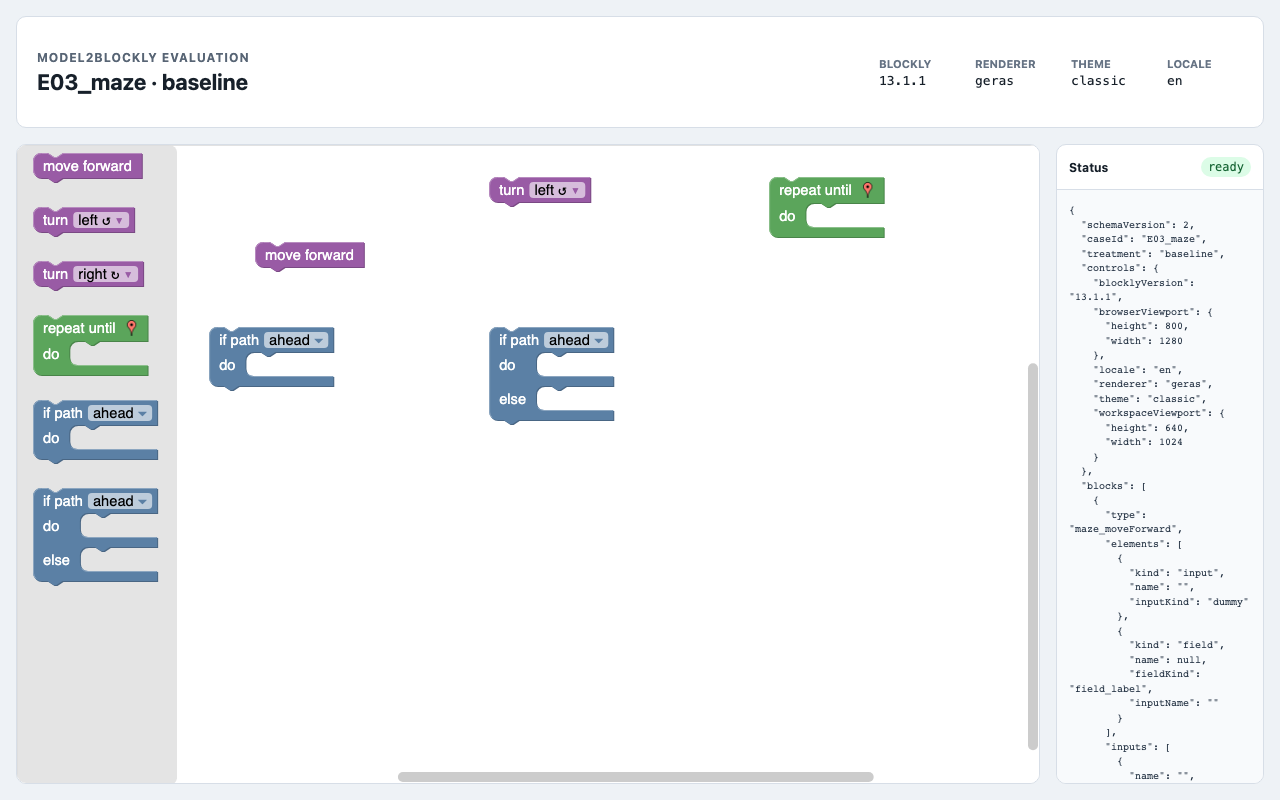
\includegraphics[width=\linewidth]{../../evaluation/official-blockly/cases/E03_maze/results/screenshots/baseline.png}
    \\[2pt]\small (a) Maze oficial
  \end{minipage}\hfill
  \begin{minipage}{0.48\textwidth}
    \centering
    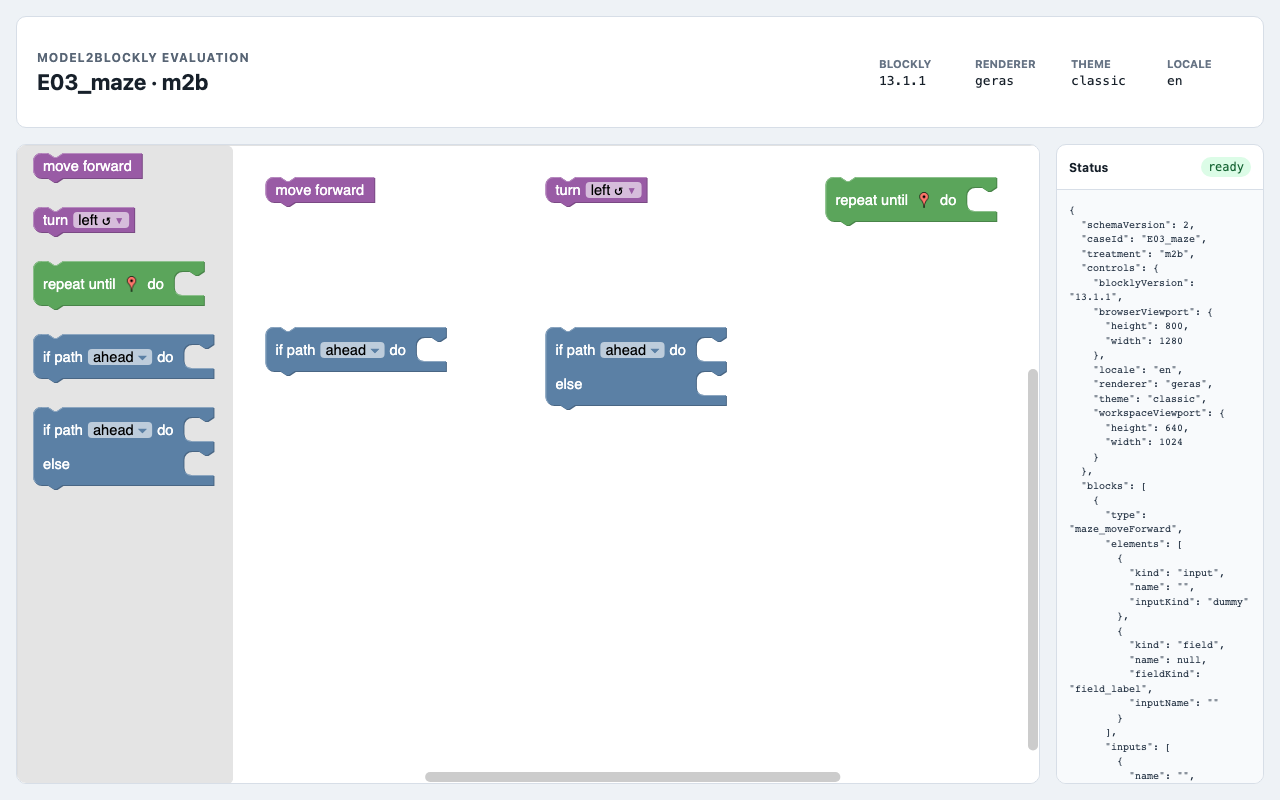
\includegraphics[width=\linewidth]{../../evaluation/official-blockly/cases/E03_maze/results/screenshots/m2b.png}
    \\[2pt]\small (b) Maze generado con M2B
  \end{minipage}

  \vspace{0.8em}

  \begin{minipage}{0.48\textwidth}
    \centering
    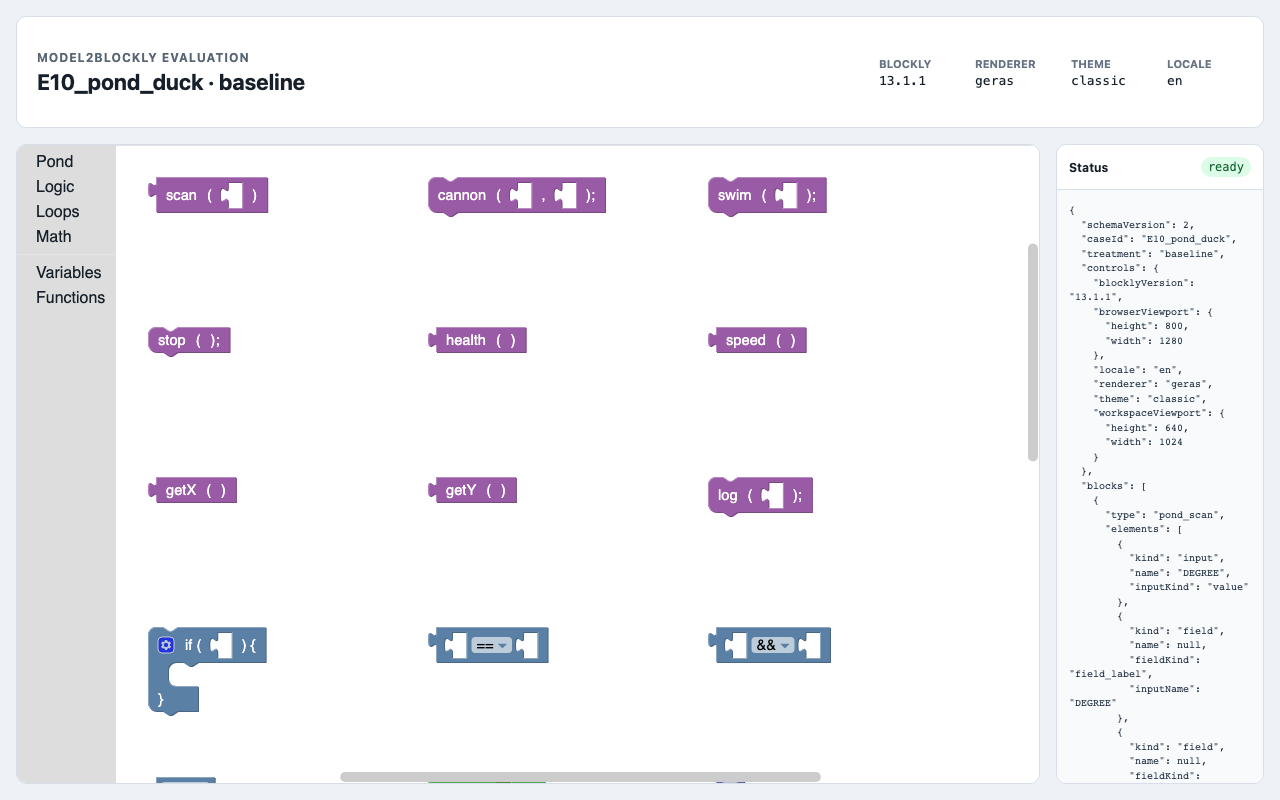
\includegraphics[width=\linewidth]{../../evaluation/official-blockly/cases/E10_pond_duck/results/screenshots/baseline.png}
    \\[2pt]\small (c) Pond oficial
  \end{minipage}\hfill
  \begin{minipage}{0.48\textwidth}
    \centering
    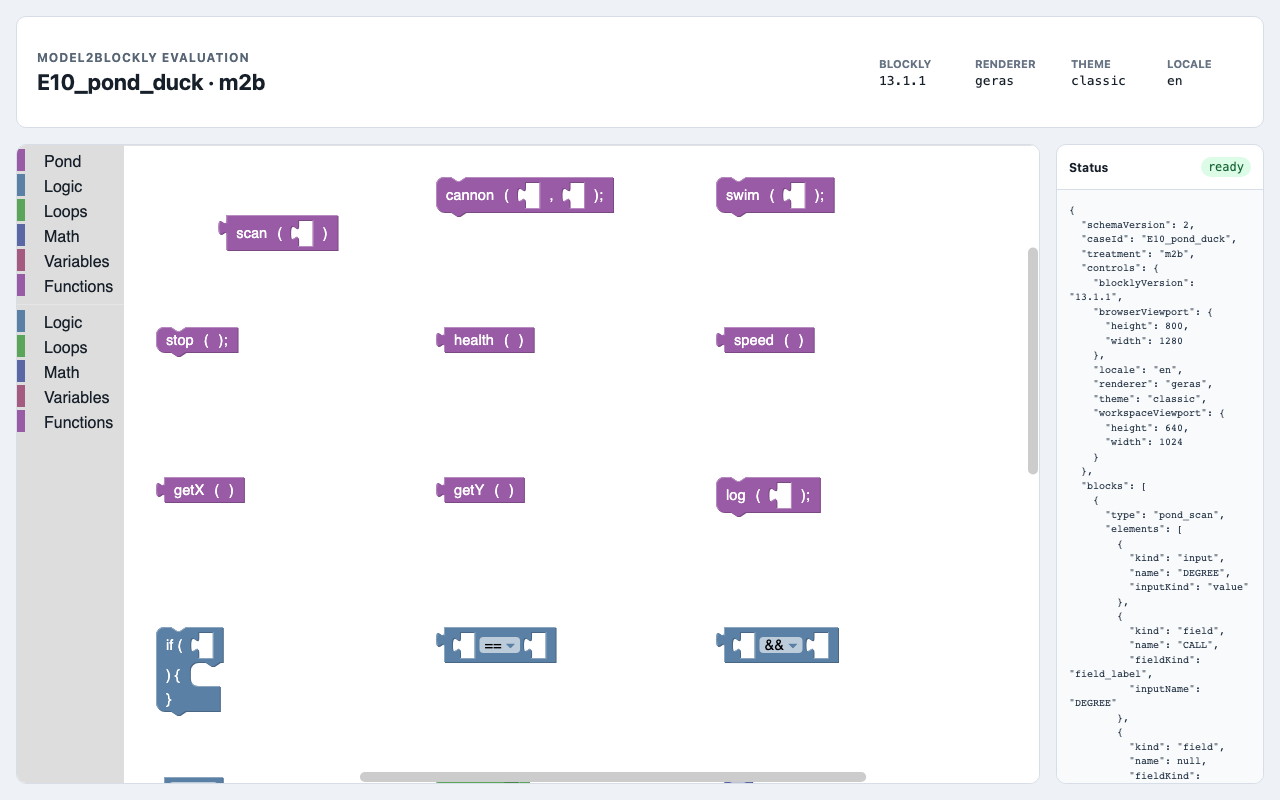
\includegraphics[width=\linewidth]{../../evaluation/official-blockly/cases/E10_pond_duck/results/screenshots/m2b.png}
    \\[2pt]\small (d) Pond generado con M2B
  \end{minipage}
  \caption{Evidencia visual auxiliar de dos casos del corpus}
  \label{fig:evidencia-visual-corpus}
\end{figure}

\subsection{Resultados de los generadores}

La paridad ponderada de los generadores es 227/291, es decir, 78,01\,\%. La
media por caso es 82,05\,\% y la mediana 83,55\,\%. Diecisiete propiedades se
marcaron como \texttt{excluded}: pertenecen al seguimiento de ejecución y a los
mecanismos de interrupción de bucles de Blockly Games, que instrumentan el
programa para la aplicación educativa, pero no definen el editor ni la
traducción básica de cada bloque.

Los resultados de Wait y Maze alcanzan el 100\,\% dentro del alcance, mientras
que Puzzle obtiene el 50\,\%. La causa principal de este último valor es que el
caso oficial serializa automáticamente el estado completo del rompecabezas,
mientras que Model2Blockly genera funciones asociadas a tipos de bloque. En los
casos Pond aparecen además procedimientos, variables y mutadores, que requieren
estado compartido durante la generación. Por tanto, la menor puntuación de esta
capa no implica que el editor no cargue; indica que la semántica de generación
oficial no siempre puede reconstruirse con el contrato actual.

\section{Resultados del esfuerzo de especificación}
\label{sec:resultados-esfuerzo}

Las diez configuraciones oficiales suman 4074 LOC no vacías y sin comentarios,
frente a 1121 LOC de los modelos \texttt{.m2b}. Aplicando la
Ecuación~\ref{eq:reduccion-loc}, la reducción ponderada es 72,48\,\%. La media de
las reducciones individuales es 73,92\,\% y la mediana 75,40\,\%. En bytes UTF-8
la reducción es semejante: de 137358 a 40563 bytes, un 70,47\,\%.

El total anterior considera cada editor como un artefacto mantenible
independiente. Para evitar que la reutilización oficial entre Pond Tutor y Pond
favorezca artificialmente a M2B, se repitió el cómputo eliminando las líneas
oficiales compartidas. El total oficial conservador pasa a 3737 LOC y la
reducción se mantiene en 70,00\,\% (67,67\,\% en bytes). Por tanto, la tendencia
no depende de contar dos veces las 337 líneas comunes.

El resultado debe interpretarse junto con la paridad funcional. Model2Blockly
reduce de forma sustancial el tamaño de la fuente mantenida, pero los modelos no
son sustitutos exactos de todas las configuraciones oficiales. El corpus
demuestra simultáneamente una reducción de esfuerzo descriptivo y un conjunto
concreto de capacidades todavía ausentes; no demuestra que pueda obtenerse el
100\,\% de cada editor con un 72,48\,\% menos de código.

\section{Límites observados en el corpus}
\label{sec:limites-corpus}

La Tabla~\ref{tab:limites-editor} agrupa las diferencias más frecuentes del
editor. El recuento se expresa en propiedades atómicas afectadas, no en número
de características independientes: una misma carencia puede afectar a varios
bloques y campos dentro de un caso.

\begin{table}[htbp]
  \centering
  \caption{Capacidades del editor que explican las diferencias principales}
  \label{tab:limites-editor}
  \resizebox{\textwidth}{!}{%
  \begin{tabular}{llrr}
    \toprule
    Capacidad & Estado predominante & Propiedades & Casos \\
    \midrule
    Políticas específicas de conexión & \texttt{unsupported} & 101 & 9 \\
    Composición avanzada de categorías & \texttt{unsupported} & 66 & 5 \\
    Entradas ficticias explícitas & \texttt{unsupported} & 52 & 4 \\
    Etiquetas de llamadas de solo lectura & \texttt{partial} & 30 & 2 \\
    Omisión intencional del color de categoría & \texttt{unsupported} & 30 & 5 \\
    Composición global de la paleta & \texttt{unsupported} & 19 & 2 \\
    Bloques preconfigurados en la paleta & \texttt{unsupported} & 19 & 7 \\
    Alineación de entradas & \texttt{unsupported} & 14 & 3 \\
    Configuración de bloques sombra & \texttt{partial} & 11 & 2 \\
    Entradas ficticias con nombre & \texttt{unsupported} & 11 & 3 \\
    Redefinición de bloques reservados & \texttt{mismatch} & 8 & 3 \\
    \bottomrule
  \end{tabular}%
  }
\end{table}

La limitación más extendida es la política de conexiones. El metamodelo común
representa si un bloque tiene salida o conexiones anterior y siguiente, pero no
todas las comprobaciones dinámicas y excepciones que los editores oficiales
añaden mediante JavaScript. También resultan difíciles las paletas construidas
programáticamente, los bloques sombra con estado inicial, la alineación visual
de entradas y las entradas ficticias usadas únicamente para controlar el
diseño. Estas características no impiden cargar el editor, aunque sí evitan una
reproducción estructural completa.

En los generadores, las diferencias más repetidas son los valores por defecto
para entradas vacías (27 propiedades en seis casos), el mapeo de enumeraciones
(10 en tres casos), la serialización automática de modelos (seis en Puzzle), la
generación sensible a mutadores (seis en Pond Tutor y Pond) y las bases de datos
de procedimientos y variables. Estas observaciones delimitan mejoras
implementables: ampliar el metamodelo de entradas y paleta, introducir políticas
de conexión declarativas y ofrecer servicios de generación con estado.

\section{Equivalencia de las rutas de entrada}
\label{sec:resultados-rutas-entrada}

RQ4 (rutas de entrada) no compara el tamaño textual de Ecore con el DSL, sino el resultado de
ambos adaptadores. Se seleccionaron Graph, Maze y Turtle para cubrir de manera
creciente campos sencillos, conexiones, menús desplegables, paletas con
categorías, espacio inicial y generadores. En los tres casos se compararon
estrictamente las siete secciones del descriptor indicadas en la
Tabla~\ref{tab:equivalencia-rutas}.

\begin{table}[htbp]
  \centering
  \caption{Equivalencia estricta entre las rutas Ecore y \texttt{.m2b}}
  \label{tab:equivalencia-rutas}
  \begin{tabular}{llll}
    \toprule
    Caso & Complejidad & Secciones comparadas & Resultado \\
    \midrule
    E01 Graph  & baja  & 7/7 & equivalente \\
    E03 Maze   & media & 7/7 & equivalente \\
    E07 Turtle & alta  & 7/7 & equivalente \\
    \bottomrule
  \end{tabular}
\end{table}

El resultado es 3/3 rutas equivalentes: controles, bloques, paleta, espacio
inicial, generadores, errores y capacidad de carga coinciden exactamente. La
prueba también resultó útil para detectar defectos de implementación. En Graph
se identificó una anotación \texttt{output} ausente en el modelo Ecore y en
Turtle se corrigió la interpretación de etiqueta y valor de los menús
desplegables por el adaptador. Tras corregir las causas, se regeneraron y
compararon de nuevo los tres pares completos. No se relajó el comparador para
hacerlos coincidir.

Este resultado muestra que, para las construcciones cubiertas, el editor
generado no depende de haber escrito el modelo mediante Xtext o mediante Ecore.
No permite afirmar equivalencia para cualquier metamodelo Ecore posible; esa
generalización requeriría ampliar el número y la diversidad de rutas evaluadas.

\section{Evidencia técnica complementaria}
\label{sec:evidencia-complementaria}

Además de la evaluación externa, el proyecto conserva pruebas orientadas a su
implementación. Los seis pares mínimos y complementarios
Ecore--\texttt{.m2b} comprueban el recorrido completo desde las dos clases de
entrada hasta un editor ejecutable y verifican variantes de controles,
conexiones, paletas y generadores. El caso Ecore específico amplía la cobertura
a construcciones sin equivalente textual. Las 145 pruebas JUnit cubren
adaptadores, validación y transformaciones, mientras que la instalación mediante
el sitio de actualización verifica el empaquetado del complemento.

Estas pruebas responden a preguntas distintas de las del corpus. Son evidencia
de regresión, integración y despliegue del sistema construido, pero no se
presentan como demostración principal de efectividad frente a editores Blockly
existentes. Del mismo modo, la capa de renderizado de una aplicación ---por
ejemplo, un laberinto, un lienzo o una simulación musical--- queda fuera de la
comparación principal: Model2Blockly genera el editor y sus generadores, no el
motor de dominio que consume el programa producido.

\section{Amenazas a la validez}
\label{sec:amenazas-validez}

\paragraph{Selección del corpus.}
Los diez casos proceden de repositorios oficiales y cubren tamaños y mecanismos
distintos, pero constituyen una muestra intencional. Los porcentajes describen
este corpus y no una población estadística de todos los editores Blockly.

\paragraph{Evolución de las dependencias.}
Los editores originales fueron desarrollados con versiones anteriores de
Blockly. Para evitar que una actualización posterior altere la comparación, se
fijaron las revisiones de las fuentes y la versión 13.1.1 de Blockly, y ambos
tratamientos se ejecutaron con el mismo contenedor de compatibilidad. El
resultado mide la configuración del editor, no la compatibilidad histórica de
cada aplicación completa.

\paragraph{Granularidad y clasificación.}
La descomposición en propiedades y los estados \texttt{partial},
\texttt{unsupported} y \texttt{excluded} requieren decisiones de modelado. Para
reducir el sesgo, el esquema se fijó con dos pilotos, cada diferencia tiene una
regla identificada y se publican tanto los conteos como los descriptores. Aun
así, otra granularidad podría cambiar los porcentajes absolutos.

\paragraph{Independencia de los artefactos.}
Pond Tutor y Pond comparten fuentes oficiales. El cálculo principal los trata
como configuraciones mantenibles diferentes y el cálculo conservador elimina
las líneas duplicadas. La reducción permanece entre el 70,00\,\% y el
72,48\,\%, lo que acota el efecto de esta dependencia.

\paragraph{Equivalencia visual y semántica.}
Las capturas no prueban igualdad visual exacta. La evaluación compara
estructuras y generadores, pero no ejecuta exhaustivamente todos los programas
posibles ni compara el comportamiento del motor de dominio. En consecuencia,
la paridad informada no debe interpretarse como equivalencia completa de las
aplicaciones Blockly Games.

\paragraph{Medida de esfuerzo.}
LOC y bytes son medidas reproducibles del tamaño de la fuente, no del tiempo de
desarrollo ni de la dificultad cognitiva. La evaluación demuestra concisión de
la especificación mantenida; un estudio con participantes sería necesario para
afirmar una reducción equivalente del tiempo o del coste humano.

\section{Respuesta a las preguntas de evaluación}
\label{sec:respuesta-rq}

\begin{table}[htbp]
  \centering
  \caption{Síntesis de las respuestas a las preguntas de evaluación}
  \label{tab:respuesta-rq}
  \footnotesize
  \begin{tabular}{L{0.24\textwidth}L{0.68\textwidth}}
    \toprule
    Pregunta de evaluación & Respuesta obtenida \\
    \midrule
    \textbf{RQ1: reproducción funcional} & Los diez editores cargan; la paridad estructural ponderada es 83,82\,\% y la de los generadores, 78,01\,\%. Todos los casos son parciales. \\
    \textbf{RQ2: esfuerzo de especificación} & M2B reduce las LOC un 72,48\,\%; al eliminar fuentes oficiales compartidas, la reducción conservadora es 70,00\,\%. \\
    \textbf{RQ3: límites} & Las principales carencias afectan a políticas de conexión, composición de paletas, entradas de presentación y generadores con estado, mutadores o serialización automática. \\
    \textbf{RQ4: rutas de entrada} & Las rutas Ecore y \texttt{.m2b} producen descriptores estrictamente equivalentes en los tres casos seleccionados (3/3). \\
    \bottomrule
  \end{tabular}
\end{table}

\section{Conclusión de la evaluación}
\label{sec:conclusion-evaluacion}

La evaluación aporta evidencia más amplia que la ejecución de un único
ejemplo. En diez editores oficiales, Model2Blockly reproduce una parte
mayoritaria de las propiedades y reduce alrededor de un 70\,\% la fuente de
configuración mantenida; la igualdad de los tres pares Ecore--\texttt{.m2b}
refuerza además la separación entre los adaptadores y la especificación común.
No existe, sin embargo, equivalencia total: todos los casos conservan
diferencias, especialmente ante paletas programáticas, mutadores o generación
con estado. Así, el corpus cuantifica la cobertura, la reducción obtenida y las
extensiones necesarias para ampliarla.

\chapter{Conclusiones y trabajo futuro}
\label{chap:conclusiones}

Este Trabajo Fin de Máster ha tratado la creación de lenguajes de dominio
específico con sintaxis basada en bloques. La motivación parte de un problema
práctico: Blockly facilita la creación de editores visuales, pero cada dominio
todavía requiere definir a mano bloques, campos, toolbox, conexiones,
validaciones y generadores. El trabajo propone una alternativa basada en
ingeniería de lenguajes y modelos: describir el dominio a alto nivel y generar
automáticamente el editor Blockly.

El capítulo se organiza en torno a los resultados y las perspectivas de la
propuesta. En primer lugar, se analiza la viabilidad del enfoque y se resumen
sus principales aportaciones. A continuación, se revisan las conclusiones
obtenidas para cada objetivo y se presentan las limitaciones identificadas.
Después se proponen posibles líneas de trabajo futuro y, finalmente, se ofrece
un cierre global del trabajo realizado.

\section{Viabilidad del enfoque}
\label{sec:viabilidad-enfoque}

El trabajo desarrollado aporta evidencia de que es viable diseñar e implementar
un entorno para la creación de lenguajes de dominio específico con sintaxis
basada en bloques. Model2Blockly acepta metamodelos Ecore enriquecidos con
anotaciones y modelos textuales \texttt{.m2b} definidos con Xtext. Ambas rutas
se transforman en un modelo intermedio común, y desde él se generan editores
Blockly ejecutables. La herramienta se materializa además como plugin Eclipse
instalable mediante un update site p2, por lo que el enfoque no queda limitado a
un prototipo ejecutado manualmente desde el código fuente.

La solución aprovecha información que ya existe en una descripción de dominio.
Las clases se convierten en tipos de bloque, los atributos en campos, las
contenciones en entradas estructurales, las referencias en desplegables
dinámicos y las cardinalidades en comprobaciones. Las anotaciones añaden
metadatos de presentación. Este proceso reduce la programación manual en
JavaScript y sigue la idea central de la ingeniería dirigida por modelos:
utilizar modelos para especificar y generar software
\cite{brambilla2017modelDriven,hutchinson2014industry}.

El trabajo también refuerza la utilidad de separar lo que el dominio significa
de la forma en que se muestra al usuario. El dominio se describe mediante Ecore
o mediante el DSL textual \texttt{.m2b}; Blockly actúa como la representación
visual generada para manipular ese dominio. Esta separación es coherente con la
forma en que los lenguajes de dominio específico organizan sus conceptos y sus
notaciones \cite{sal2024dsl}.

\section{Principales aportaciones}
\label{sec:aportaciones}

La primera aportación es una arquitectura generativa que conecta Ecore,
\texttt{.m2b}, \texttt{EditorSpec} y Blockly. La arquitectura introduce un
modelo intermedio, en lugar de acoplar directamente cada entrada a una salida
concreta. Las dos rutas se normalizan hacia el mismo contrato y no requieren
generadores separados.

La segunda aportación es el modelo intermedio común. Este
modelo recoge los elementos necesarios para construir un editor visual: bloques,
campos, categorías, entradas de valor, entradas de sentencias, referencias,
validaciones, opciones de workspace y metadatos de código. También define el
contrato entre adaptadores y generadores, se serializa como XMI y se recarga
antes de generar la salida final.

La tercera aportación es la ruta Ecore. El adaptador desarrollado permite partir
de un metamodelo y derivar una especificación de editor. Esta ruta cubre
la parte metamodelo-céntrica del sistema: usar un metamodelo, enriquecido cuando
sea necesario con anotaciones, para generar código basado en Blockly.

La cuarta aportación es la ruta textual \texttt{.m2b}. Esta ruta facilita definir
lenguajes de bloques de forma compacta, con una sintaxis cercana a los conceptos
que después se convertirán en bloques. También incorpora validación estática
mediante Xtext, lo que permite detectar errores antes de generar el editor cuando
se usa esta forma de autoría.

La quinta aportación es la generación de editores ejecutables. La salida
HTML/JavaScript produce definiciones de bloques, toolbox, generadores,
validaciones, páginas HTML autocontenidas, exportación JSON/XMI, informes de
generación, modelos de ejemplo y una vista Blockly de las reglas de validación.

La sexta aportación es la integración práctica de la herramienta. El plugin
Eclipse ofrece comandos para generar desde ficheros \texttt{.m2b} y
\texttt{.ecore}, y para aplicar de vuelta a la fuente cambios soportados en las
reglas visuales de validación. El update site y las demos publicadas facilitan la
revisión externa del resultado.

Finalmente, el trabajo aporta una evaluación basada en un ejemplo conductor y
pruebas automáticas. AppMaker se describe como metamodelo Ecore anotado y como
fichero textual \texttt{.m2b}, lo que permite comparar las dos formas de autoría.
Las 144 pruebas JUnit organizadas por capa aportan evidencia adicional sobre el
comportamiento del modelo intermedio, los adaptadores y los generadores.

\section{Conclusiones por objetivos}
\label{sec:conclusiones-objetivos}

Los objetivos específicos definidos al inicio del trabajo se han abordado de la
siguiente forma:

\begin{itemize}
  \item \textbf{OE1.} Se analizaron los elementos necesarios para un editor de
  bloques y se representaron explícitamente en el modelo intermedio: tipos de
  bloque, campos, conexiones, categorías, referencias, validaciones y
  generación.
  \item \textbf{OE2.} Se implementó una ruta Ecore que transforma clases,
  atributos, referencias, herencia, cardinalidades y anotaciones en una
  especificación Blockly.
  \item \textbf{OE3.} Se definió una ruta textual \texttt{.m2b} con Xtext para
  describir lenguajes de bloques sin editar directamente ficheros Ecore en
  ejemplos o configuraciones compactas.
  \item \textbf{OE4.} Se diseñó e implementó un modelo intermedio común como
  representación común independiente de la fuente de entrada.
  \item \textbf{OE5.} Se generaron editores HTML/JavaScript ejecutables con
  bloques, toolbox, validaciones, guardado, carga, exportación JSON/XMI e
  informes de generación.
  \item \textbf{OE6.} Se incorporaron comprobaciones, referencias dinámicas,
  personalización visual, metadatos de interfaz, plantillas de código y una
  vista Blockly editable para reglas de validación.
  \item \textbf{OE7.} Se evaluó la solución con AppMaker por la ruta Ecore y por
  la ruta textual \texttt{.m2b}, junto con pruebas automáticas sobre las capas
  principales del sistema.
\end{itemize}

Por lo tanto, el enfoque es técnicamente viable dentro del alcance definido.
Un dominio descrito con Ecore anotado o con \texttt{.m2b} puede transformarse en
un editor de bloques mediante una cadena generativa reproducible. La ruta
textual muestra además que esa información puede escribirse de forma más
compacta y normalizarse hacia el mismo modelo intermedio.

\section{Limitaciones}
\label{sec:conclusiones-limitaciones}

Aunque los resultados respaldan el enfoque principal, el trabajo tiene
limitaciones. La primera es que la evaluación usa un ejemplo diseñado dentro del
proyecto. AppMaker cubre estructuras variadas, pero no equivale a una validación
industrial con muchos metamodelos externos. Por ello, el caso estudiado apoya la
viabilidad de la herramienta, pero no prueba su generalidad de forma exhaustiva.

La segunda limitación afecta a las validaciones. Model2Blockly genera advertencias
para mínimos y máximos de bloques, campos obligatorios, referencias obligatorias,
unicidad, reglas simples de orden, expresiones declaradas en anotaciones y un
subconjunto sencillo de invariantes OCL. Este soporte cubre restricciones
frecuentes, pero no equivale a un lenguaje completo de restricciones como OCL
\cite{omgOcl}. No se soportan invariantes arbitrarios, cuantificadores,
navegación compleja ni análisis semántico profundo. Además, las comprobaciones
generadas producen advertencias, no una validación bloqueante. La edición visual
de reglas tampoco es una transformación bidireccional general: solo se aplican de
vuelta a la fuente los cambios que tienen una correspondencia clara.

La tercera limitación se refiere a las referencias. Las referencias no
contenidas se representan mediante desplegables dinámicos, lo que permite
seleccionar elementos existentes del workspace. Además, el runtime HTML
sincroniza referencias opuestas no contenidas cuando ambos extremos son
editables. La limitación actual está en los casos más complejos: referencias
opuestas con semántica de contenedor y visualización avanzada de relaciones
entre elementos.

La cuarta limitación está relacionada con la generación de código. La solución
incluye plantillas de código y una representación textual por defecto, pero no
incorpora todavía formateadores específicos, análisis de tipos avanzado,
gestión de imports, generación multiarchivo ni integración directa con
herramientas externas de construcción o ejecución.

La quinta limitación es de evaluación de usuario. Este TFM no mide si los
editores generados reducen efectivamente el esfuerzo de aprendizaje o mejoran la
experiencia de usuarios no técnicos. La literatura sobre programación por
bloques muestra que la modalidad de interacción influye en las prácticas de los
usuarios noveles \cite{weintrop2018modalities}, pero validar empíricamente los
editores generados requeriría un estudio específico.

\section{Trabajo futuro}
\label{sec:trabajo-futuro}

A partir de estas limitaciones se identifican varias líneas de trabajo futuro.

En primer lugar, sería útil ampliar el soporte de validación. Una opción sería
integrar un lenguaje de restricciones más expresivo o un mecanismo de reglas
declarativas. Así se podrían describir condiciones más complejas que los mínimos,
máximos y reglas de orden inmediato. Esta línea también permitiría ampliar la
traducción entre reglas visuales editadas y su representación en
\texttt{.m2b} o en anotaciones Ecore.

En segundo lugar, la gestión de referencias podría evolucionar hacia un soporte
más completo de referencias bidireccionales. Esto implicaría extender la
sincronización de referencias opuestas en el runtime HTML, cubrir casos de
contenedor, detectar referencias que apuntan a elementos ya eliminados y ofrecer
visualizaciones más claras de las relaciones entre elementos del workspace.

En tercer lugar, se podría profundizar en la importación y exportación de
modelos. Actualmente la herramienta se centra en generar editores y exportar el
contenido del workspace. Una línea futura consistiría en importar modelos XMI
existentes y reconstruir automáticamente el workspace Blockly correspondiente.
Esto acercaría más la herramienta a flujos completos de ingeniería de modelos.

En cuarto lugar, la generación de código podría enriquecerse. Las plantillas
actuales son suficientes para demostrar una ruta genérica de exportación, pero
podrían ampliarse con validación de plantillas, tipado, formateadores,
generación multiarchivo y objetivos específicos para lenguajes o plataformas
concretas.

En quinto lugar, podrían explorarse interfaces web más avanzadas sobre el mismo
modelo intermedio. Un futuro objetivo de generación podría incorporar un
inspector estructurado, temas visuales por dominio, componentes personalizados y
modos de edición más adaptados a usuarios finales.

En sexto lugar, sería conveniente realizar una evaluación empírica con usuarios.
Un estudio futuro podría comparar el esfuerzo necesario para construir un editor
Blockly manualmente frente al uso de Model2Blockly, o analizar cómo interactúan
usuarios no técnicos con editores generados para distintos dominios. Esta
evaluación permitiría complementar la evidencia técnica de este TFM con datos
de uso.

Por último, convendría robustecer el ciclo de publicación del plugin. La versión
actual ya dispone de update site p2 y verificaciones de empaquetado, pero una
línea futura sería automatizar más la publicación, el versionado y las pruebas de
instalación sobre instalaciones limpias de Eclipse.

\section{Cierre}
\label{sec:cierre}

Model2Blockly aporta evidencia de que es posible conectar técnicas de ingeniería de
lenguajes con entornos de programación basada en bloques. El resultado no es un
único editor visual, sino una infraestructura que transforma descripciones de
dominio en editores Blockly ejecutables. El conocimiento del dominio se mantiene
en modelos o DSLs de alto nivel, y la sintaxis visual se genera a partir de ellos.

El trabajo muestra que la combinación de Ecore, Xtext, un modelo intermedio EMF,
generación HTML/JavaScript y Blockly es viable para construir editores de
lenguajes de dominio específico con sintaxis basada en bloques. Dentro del
alcance definido, esta combinación es una alternativa razonable a la programación
manual de editores Blockly y deja una base extensible para trabajos futuros.


\printbibliography

\end{document}
